% Формат А4, 14pt (ГОСТ Р 7.0.11-2011, 5.3.6)
\documentclass[a4paper,14pt]{extreport}

%%%%%%%%%%%%%%%%%%%%%%%%%%%%%%%%%%%%%%%%%%%%%%%%%%%%%%
%%%% Файл упрощённых настроек шаблона диссертации %%%%
%%%%%%%%%%%%%%%%%%%%%%%%%%%%%%%%%%%%%%%%%%%%%%%%%%%%%%

%%%        Подключение пакетов                 %%%
\usepackage{ifthen}                 % добавляет ifthenelse
%%% Инициализирование переменных, не трогать!  %%%
\newcounter{bibliosel}
\newcounter{tabcap}
\newcounter{tablaba}
\newcounter{tabtita}

%%%%%%%%%%%%%%%%%%%%%%%%%%%%%%%%%%%%%%%%%%%%%%%%%%

%%% Область упрощённого управления оформлением %%%

%% Библиография
\setcounter{bibliosel}{0}           % 0 --- встроенная реализация с загрузкой файла через движок bibtex8; 1 --- реализация пакетом biblatex через движок biber

%% Подпись таблиц
\setcounter{tabcap}{0}              % 0 --- по ГОСТ, номер таблицы и название разделены тире, выровнены по левому краю, при необходимости на нескольких строках; 1 --- подпись таблицы не по ГОСТ, на двух и более строках, дальнейшие настройки: 
%Выравнивание первой строки, с подписью и номером
\setcounter{tablaba}{2}             % 0 --- по левому краю; 1 --- по центру; 2 --- по правому краю
%Выравнивание строк с самим названием таблицы
\setcounter{tabtita}{1}             % 0 --- по левому краю; 1 --- по центру; 2 --- по правому краю

               % Упрощённые настройки шаблона 

%%% Проверка используемого TeX-движка %%%
\usepackage{iftex}
\newif\ifxetexorluatex   % определяем новый условный оператор (http://tex.stackexchange.com/a/47579/79756)
\ifXeTeX
    \xetexorluatextrue
\else
    \ifLuaTeX
        \xetexorluatextrue
    \else
        \xetexorluatexfalse
    \fi
\fi

%%% Поля и разметка страницы %%%
\usepackage{pdflscape}                              % Для включения альбомных страниц
\usepackage{geometry}                               % Для последующего задания полей

%%% Математические пакеты %%%
\usepackage{amsthm,amsfonts,amsmath,amssymb,amscd}  % Математические дополнения от AMS
\usepackage{mathtools}                              % Добавляет окружение multlined

%%%% Установки для размера шрифта 14 pt %%%%
%% Формирование переменных и констант для сравнения (один раз для всех подключаемых файлов)%%
%% должно располагаться до вызова пакета fontspec или polyglossia, потому что они сбивают его работу
\newlength{\curtextsize}
\newlength{\bigtextsize}
\setlength{\bigtextsize}{13.9pt}

\makeatletter
%\show\f@size                                       % неплохо для отслеживания, но вызывает стопорение процесса, если документ компилируется без команды  -interaction=nonstopmode 
\setlength{\curtextsize}{\f@size pt}
\makeatother

%%% Кодировки и шрифты %%%
\ifxetexorluatex
    \usepackage{polyglossia}                        % Поддержка многоязычности (fontspec подгружается автоматически)
\else
    \RequirePDFTeX                                  % tests for PDFTEX use and throws an error if a different engine is being used
    \usepackage{cmap}                               % Улучшенный поиск русских слов в полученном pdf-файле
    \usepackage[T2A]{fontenc}                       % Поддержка русских букв
    \usepackage[utf8]{inputenc}                     % Кодировка utf8
    \usepackage[english, russian]{babel}            % Языки: русский, английский
    \IfFileExists{pscyr.sty}{\usepackage{pscyr}}{}  % Красивые русские шрифты
\fi

%%% Оформление абзацев %%%
\usepackage{indentfirst}                            % Красная строка

%%% Цвета %%%
%\usepackage[dvipsnames,usenames]{xcolor}
\usepackage[usenames,dvipsnames]{xcolor}
\usepackage{colortbl}


%%% Таблицы %%%
\usepackage{longtable}                              % Длинные таблицы
\usepackage{multirow,makecell,array}                % Улучшенное форматирование таблиц
\usepackage{booktabs}                               % Возможность оформления таблиц в классическом книжном стиле (при правильном использовании не противоречит ГОСТ)

%%% Общее форматирование
\usepackage{soulutf8}                               % Поддержка переносоустойчивых подчёркиваний и зачёркиваний
\usepackage{icomma}                                 % Запятая в десятичных дробях


%%% Гиперссылки %%%
\usepackage{hyperref}

%%% Изображения %%%
\usepackage{graphicx}                               % Подключаем пакет работы с графикой

%%% Списки %%%
\usepackage{enumitem}

%%% Подписи %%%
\usepackage{caption}                                % Для управления подписями (рисунков и таблиц) % Может управлять номерами рисунков и таблиц с caption %Иногда может управлять заголовками в списках рисунков и таблиц
\usepackage{subcaption}                             % Работа с подрисунками и подобным

%%% Интервалы %%%
\usepackage[onehalfspacing]{setspace}               % Опция запуска пакета правит не только интервалы в обычном тексте, но и формульные

%%% Счётчики %%%
\usepackage[figure,table]{totalcount}               % Счётчик рисунков и таблиц
\usepackage{totcount}                               % Пакет создания счётчиков на основе последнего номера подсчитываемого элемента (может требовать дважды компилировать документ)
\usepackage{totpages}                               % Счётчик страниц, совместимый с hyperref (ссылается на номер последней страницы). Желательно ставить последним пакетом в преамбуле

\usepackage{tabularx}
  % Пакеты общие для диссертации и автореферата
%%% Колонтитулы %%%
\usepackage{fancyhdr}

%%% Прикладные пакеты %%% 
\usepackage{calc}               % Пакет для расчётов параметров, например длины
%\usepackage{etoolbox}          % ради функции patchcmd для управления списком литературы

\usepackage {interfaces-base}   % Набор базовых интерфейсов к некоторым пакетам, конкретные реализации загружаются в стиле

%%% Заголовки %%%
\usepackage{titlesec}           % Пакет настройки шрифтов заголовков в тексте

%%% Оглавление %%%
\usepackage{tocloft}

%%% Счётчики %%%
\usepackage{chngcntr}           % оперативная перенастройка счётчиков

\usepackage{floatrow}

\usepackage{tikz}
%\usetikzlibrary{arrows,positioning}
\usetikzlibrary{shapes.geometric, calc}%,calc,chains}

%\usetikzlibrary{arrows.meta}

% \usepackage{tikz}
% \usetikzlibrary{external}
% \tikzexternalize
% % 
%  \usetikzlibrary{arrows,positioning}
%  \usetikzlibrary{shapes.geometric,calc,chains}
% \usetikzlibrary{arrows.meta}         % Пакеты для диссертации
\usepackage{tabularx,tabulary}  %таблицы с автоматически подбирающейся шириной столбцов

% Листинги с исходным кодом программ
\usepackage{fancyvrb}
\usepackage{listings}

% Плавающие окружения. во многом лучше пакета float
\usepackage{floatrow}
        % Пакеты для специфических пользовательских задач
%%% Переопределение именований, чтобы можно было и в преамбуле использовать %%%
\renewcommand{\chaptername}{Глава}
\renewcommand{\appendixname}{Приложение} % (ГОСТ Р 7.0.11-2011, 5.7)
       % Переопределение именований, чтобы можно было и в преамбуле использовать
%%% Макет страницы %%%
% Выставляем значения полей (ГОСТ 7.0.11-2011, 5.3.7)
\geometry{a4paper,top=2cm,bottom=2cm,left=2.5cm,right=1cm}

%%% Кодировки и шрифты %%%
\ifxetexorluatex
    \setmainlanguage[babelshorthands=true]{russian}  % Язык по-умолчанию русский с поддержкой приятных команд пакета babel
    \setotherlanguage{english}                       % Дополнительный язык = английский (в американской вариации по-умолчанию)
    \ifXeTeX
        \defaultfontfeatures{Ligatures=TeX,Mapping=tex-text}
    \else
        \defaultfontfeatures{Ligatures=TeX}
    \fi
    \setmainfont{Times New Roman}
    \newfontfamily\cyrillicfont{Times New Roman}
    \setsansfont{Arial}
    \newfontfamily\cyrillicfontsf{Arial}
    \setmonofont{Courier New}
    \newfontfamily\cyrillicfonttt{Courier New}
\else
    \IfFileExists{pscyr.sty}{\renewcommand{\rmdefault}{ftm}}{}
\fi

%%% Интервалы %%%
%linespread-реализация ближе к реализации полуторного интервала в ворде.
%setspace реализация заточена под шрифты 10, 11, 12pt, под остальные кегли хуже, но всё же ближе к типографской классике. 
\linespread{1.3}                    % Полуторный интервал (ГОСТ Р 7.0.11-2011, 5.3.6)

%%% Выравнивание и переносы %%%
\sloppy                             % Избавляемся от переполнений
\clubpenalty=10000                  % Запрещаем разрыв страницы после первой строки абзаца
\widowpenalty=10000                 % Запрещаем разрыв страницы после последней строки абзаца

%%% Изображения %%%
\graphicspath{{images/}}            % Пути к изображениям

%%% Подписи %%%
\captionsetup{%
singlelinecheck=off,                % Многострочные подписи, например у таблиц
skip=2pt,                           % Вертикальная отбивка между подписью и содержимым рисунка или таблицы определяется ключом
justification=centering,            % Центрирование подписей, заданных командой \caption
}

%%% Рисунки %%%
\DeclareCaptionLabelSeparator*{emdash}{~--- }             % (ГОСТ 2.105, 4.3.1)
\captionsetup[figure]{labelsep=emdash,font=onehalfspacing,position=bottom}

%%% Таблицы %%%
\ifthenelse{\equal{\thetabcap}{0}}{%
    \newcommand{\tabcapalign}{\raggedright}  % по левому краю страницы или аналога parbox
}

\ifthenelse{\equal{\thetablaba}{0} \AND \equal{\thetabcap}{1}}{%
    \newcommand{\tabcapalign}{\raggedright}  % по левому краю страницы или аналога parbox
}

\ifthenelse{\equal{\thetablaba}{1} \AND \equal{\thetabcap}{1}}{%
    \newcommand{\tabcapalign}{\centering}    % по центру страницы или аналога parbox
}

\ifthenelse{\equal{\thetablaba}{2} \AND \equal{\thetabcap}{1}}{%
    \newcommand{\tabcapalign}{\raggedleft}   % по правому краю страницы или аналога parbox
}

\ifthenelse{\equal{\thetabtita}{0} \AND \equal{\thetabcap}{1}}{%
    \newcommand{\tabtitalign}{\raggedright}  % по левому краю страницы или аналога parbox
}

\ifthenelse{\equal{\thetabtita}{1} \AND \equal{\thetabcap}{1}}{%
    \newcommand{\tabtitalign}{\centering}    % по центру страницы или аналога parbox
}

\ifthenelse{\equal{\thetabtita}{2} \AND \equal{\thetabcap}{1}}{%
    \newcommand{\tabtitalign}{\raggedleft}   % по правому краю страницы или аналога parbox
}

\ifthenelse{\equal{\thetabcap}{0}}{%
    \DeclareCaptionFormat{tablecaption}{\tabcapalign #1#2#3}
    \DeclareCaptionFormat{tablenocaption}{\tabcapalign #1#2}    % Наименование таблицы отсутствует
    \captionsetup[table]{labelsep=emdash}                       % тире как разделитель идентификатора с номером от наименования
}{%
    \DeclareCaptionFormat{tablecaption}{\tabcapalign #1#2\par%  % Идентификатор таблицы на отдельной строке
        \tabtitalign{#3}}                                       % Наименование таблицы строкой ниже
    \DeclareCaptionFormat{tablenocaption}{\tabcapalign #1#2}    % Наименование таблицы отсутствует
    \captionsetup[table]{labelsep=space}                        % пробельный разделитель идентификатора с номером от наименования
}
\captionsetup[table]{format=tablecaption,singlelinecheck=off,font=onehalfspacing,position=top,skip=0pt}  % многострочные наименования и прочее
\DeclareCaptionLabelFormat{continued}{Продолжение таблицы~#2}

%%% Подписи подрисунков %%%
\renewcommand{\thesubfigure}{\asbuk{subfigure}}           % Буквенные номера подрисунков
\captionsetup[subfigure]{font={normalsize},               % Шрифт подписи названий подрисунков (не отличается от основного)
    labelformat=brace,                                    % Формат обозначения подрисунка
    justification=centering,                              % Выключка подписей (форматирование), один из вариантов            
}
%\DeclareCaptionFont{font12pt}{\fontsize{12pt}{13pt}\selectfont} % объявляем шрифт 12pt для использования в подписях, тут же надо интерлиньяж объявлять, если не наследуется
%\captionsetup[subfigure]{font={font12pt}}                 % Шрифт подписи названий подрисунков (всегда 12pt)

%%% Цвета гиперссылок %%%
\definecolor{linkcolor}{rgb}{0.0,0,0.9} % 0.9,0,0
\definecolor{citecolor}{rgb}{0,0.6,0}
\definecolor{urlcolor}{rgb}{0,0,1}

%%% Настройки гиперссылок %%%
\hypersetup{
    linktocpage=true,           % ссылки с номера страницы в оглавлении, списке таблиц и списке рисунков
%    pdfpagelabels=false,        % set PDF page labels (true|false)
    plainpages=false,           % Forces page anchors to be named by the Arabic form  of the page number, rather than the formatted form
    colorlinks,                 % ссылки отображаются раскрашенным текстом, а не раскрашенным прямоугольником, вокруг текста
    linkcolor={linkcolor},      % цвет ссылок типа ref, eqref и подобных
    citecolor={citecolor},      % цвет ссылок-цитат
    urlcolor={urlcolor},        % цвет гиперссылок
}

\ifLuaTeX
    \hypersetup{
        unicode,                % Unicode encoded PDF strings
    }
\fi

%%% Шаблон %%%
\DeclareRobustCommand{\todo}{\textcolor{red}}       % решаем проблему превращения названия цвета в результате \MakeUppercase, http://tex.stackexchange.com/a/187930/79756 , \DeclareRobustCommand protects \todo from expanding inside \MakeUppercase
\setlength{\parindent}{2.5em}                       % Абзацный отступ. Должен быть одинаковым по всему тексту и равен пяти знакам (ГОСТ Р 7.0.11-2011, 5.3.7).

%%% Списки %%%
% Используем дефис для ненумерованных списков (ГОСТ 2.105-95, 4.1.7)
\renewcommand{\labelitemi}{\normalfont\bfseries{--}} 
\setlist{nosep,%                                    % Единый стиль для всех списков (пакет enumitem), без дополнительных интервалов.
    labelindent=\parindent,leftmargin=*%            % Каждый пункт, подпункт и перечисление записывают с абзацного отступа (ГОСТ 2.105-95, 4.1.8)
}
    % Стили общие для диссертации и автореферата
\LoadInterface {titlesec}                   % Подгружаем интерфейсы для дополнительных опций управления некоторыми пакетами

%%% Блок управления параметрами для выравнивания заголовков в тексте %%%
\newlength{\otstuplen}
\setlength{\otstuplen}{\theotstup\parindent}
\ifthenelse{\equal{\theheadingalign}{0}}{% выравнивание заголовков в тексте
    \newcommand{\hdngalign}{\filcenter}                % по центру
    \newcommand{\hdngaligni}{\hfill\hspace{\otstuplen}}% по центру
}{%
    \newcommand{\hdngalign}{\filright}                 % по левому краю
    \newcommand{\hdngaligni}{\hspace{\otstuplen}}      % по левому краю
} % В обоих случаях вроде бы без переноса, как и надо (ГОСТ Р 7.0.11-2011, 5.3.5)

%%% Оглавление %%%
\renewcommand{\cftchapdotsep}{\cftdotsep}                % отбивка точками до номера страницы начала главы/раздела
\renewcommand{\cfttoctitlefont}{\hdngaligni\fontsize{14pt}{16pt}\selectfont\bfseries}% вместе со следующей строкой
\renewcommand{\cftaftertoctitle}{\hfill}                 % устанавливает заголовок по центру
\setlength{\cftbeforetoctitleskip}{-1.4\curtextsize}     % Поскольку этот заголовок всегда является первым на странице, то перед ним отделять пустым тройным интервалом не следует. Независимо от основного шрифта, в этом случае зануление (почти) происходит при -1.4\curtextsize.
\setlength{\cftaftertoctitleskip}{\theintvl\curtextsize} % Если считаем Оглавление заголовком, то выставляем после него тройной интервал через наше определённое значение

%% Переносить слова в заголовке не допускается (ГОСТ Р 7.0.11-2011, 5.3.5). Заголовки в оглавлении должны точно повторять заголовки в тексте (ГОСТ Р 7.0.11-2011, 5.2.3). Прямого указания на запрет переносов в оглавлении нет, но по той же логике невнесения искажений в смысл, лучше в оглавлении не переносить:
\cftsetrmarg{2.55em plus1fil}                       %To have the (sectional) titles in the ToC, etc., typeset ragged right with no hyphenation
\renewcommand{\cftchappagefont}{\normalfont}        % нежирные номера страниц у глав в оглавлении
\renewcommand{\cftchapleader}{\cftdotfill{\cftchapdotsep}}% нежирные точки до номеров страниц у глав в оглавлении
%\renewcommand{\cftchapfont}{}                       % нежирные названия глав в оглавлении

\ifthenelse{\theheadingdelim > 0}{%
    \renewcommand\cftchapaftersnum{.\ }   % добавляет точку с пробелом после номера раздела в оглавлении
}{%
\renewcommand\cftchapaftersnum{\quad}     % добавляет \quad после номера раздела в оглавлении
}
\ifthenelse{\theheadingdelim > 1}{%
    \renewcommand\cftsecaftersnum{.\ }    % добавляет точку с пробелом после номера подраздела в оглавлении
    \renewcommand\cftsubsecaftersnum{.\ } % добавляет точку с пробелом после номера подподраздела в оглавлении
}{%
\renewcommand\cftsecaftersnum{\quad}      % добавляет \quad после номера подраздела в оглавлении
\renewcommand\cftsubsecaftersnum{\quad}   % добавляет \quad после номера подподраздела в оглавлении
}

\ifthenelse{\equal{\thepgnum}{1}}{%
    \addtocontents{toc}{~\hfill{Стр.}\par}% добавить Стр. над номерами страниц
}

%%% Оформление названий глав %%%
%% настройки заголовка списка рисунков
\renewcommand{\cftloftitlefont}{\hdngaligni\fontsize{14pt}{16pt}\selectfont\bfseries}% вместе со следующей строкой
\renewcommand{\cftafterloftitle}{\hfill}                                             % устанавливает заголовок по центру
\setlength{\cftbeforeloftitleskip}{-1.5\curtextsize}     % Поскольку этот заголовок всегда является первым на странице, то перед ним отделять пустым тройным интервалом не следует. Независимо от основного шрифта, в этом случае зануление (почти) происходит при -1.5\curtextsize.
\setlength{\cftafterloftitleskip}{\theintvl\curtextsize} % выставляем после него тройной интервал через наше определённое значение

%% настройки заголовка списка таблиц
\renewcommand{\cftlottitlefont}{\hdngaligni\fontsize{14pt}{16pt}\selectfont\bfseries}% вместе со следующей строкой
\renewcommand{\cftafterlottitle}{\hfill}                                             % устанавливает заголовок по центру
\setlength{\cftbeforelottitleskip}{-1.5\curtextsize}     % Поскольку этот заголовок всегда является первым на странице, то перед ним отделять пустым тройным интервалом не следует. Независимо от основного шрифта, в этом случае зануление (почти) происходит при -1.5\curtextsize.
\setlength{\cftafterlottitleskip}{\theintvl\curtextsize} % выставляем после него тройной интервал через наше определённое значение

\ifnum\curtextsize>\bigtextsize     % Проверяем условие использования базового шрифта 14 pt
\setlength{\headheight}{17pt}       % Исправляем высоту заголовка
\else
\setlength{\headheight}{15pt}       % Исправляем высоту заголовка
\fi

%%% Колонтитулы %%%
% Порядковый номер страницы печатают на середине верхнего поля страницы (ГОСТ Р 7.0.11-2011, 5.3.8)
\makeatletter
\let\ps@plain\ps@fancy              % Подчиняем первые страницы каждой главы общим правилам
\makeatother
\pagestyle{fancy}                   % Меняем стиль оформления страниц
\fancyhf{}                          % Очищаем текущие значения
\fancyhead[C]{\thepage}             % Печатаем номер страницы на середине верхнего поля
\renewcommand{\headrulewidth}{0pt}  % Убираем разделительную линию

%%% Оформление заголовков глав, разделов, подразделов %%%
%% Работа должна быть выполнена ... размером шрифта 12-14 пунктов (ГОСТ Р 7.0.11-2011, 5.3.8). То есть не должно быть надписей шрифтом более 14. Так и поставим.
%% Эти установки будут давать одинаковый результат независимо от выбора базовым шрифтом 12 пт или 14 пт
\titleformat{\chapter}[block]                                % default display;  hang = with a hanging label. (Like the standard \section.); block = typesets the whole title in a block (a paragraph) without additional formatting. Useful in centered titles
        {\hdngalign\fontsize{14pt}{16pt}\selectfont\bfseries}% 
        %\fontsize{<size>}{<skip>} % второе число ставим 1.2*первое, чтобы адекватно отрабатывали команды по расчету полуторного интервала (домножая разные комбинации коэффициентов на этот)
        {\thechapter\cftchapaftersnum}                       % Заголовки в оглавлении должны точно повторять заголовки в тексте (ГОСТ Р 7.0.11-2011, 5.2.3).
        {0em}% отступ от номера до текста
        {}%

\titleformat{\section}[block]                                % default hang;  hang = with a hanging label. (Like the standard \section.); block = typesets the whole title in a block (a paragraph) without additional formatting. Useful in centered titles
        {\hdngalign\fontsize{14pt}{16pt}\selectfont\bfseries}% 
        %\fontsize{<size>}{<skip>} % второе число ставим 1.2*первое, чтобы адекватно отрабатывали команды по расчету полуторного интервала (домножая разные комбинации коэффициентов на этот)
        {\thesection\cftsecaftersnum}                        % Заголовки в оглавлении должны точно повторять заголовки в тексте (ГОСТ Р 7.0.11-2011, 5.2.3).
        {0em}% отступ от номера до текста
        {}%

\titleformat{\subsection}[block]                             % default hang;  hang = with a hanging label. (Like the standard \section.); block = typesets the whole title in a block (a paragraph) without additional formatting. Useful in centered titles
        {\hdngalign\fontsize{14pt}{16pt}\selectfont\bfseries}% 
        %\fontsize{<size>}{<skip>} % второе число ставим 1.2*первое, чтобы адекватно отрабатывали команды по расчету полуторного интервала (домножая разные комбинации коэффициентов на этот)
        {\thesubsection\cftsubsecaftersnum}                  % Заголовки в оглавлении должны точно повторять заголовки в тексте (ГОСТ Р 7.0.11-2011, 5.2.3).
        {0em}% отступ от номера до текста
        {}%

\ifthenelse{\equal{\thechapstyle}{1}}{%
    \sectionformat{\chapter}{% Параметры заголовков разделов в тексте
        label=\chaptername\ \thechapter\cftchapaftersnum,
        labelsep=0em,
    }
    %% Следующие две строки: будет вписано слово Глава перед каждым номером раздела в оглавлении   
    \renewcommand{\cftchappresnum}{\chaptername\ }
    \setlength{\cftchapnumwidth}{\widthof{\cftchapfont\cftchappresnum\thechapter\cftchapaftersnum}}
}%

%% Интервалы между заголовками
% На эти величины titlespacing множит через *
\beforetitleunit=\curtextsize% привязались к нашему размеру шрифта
\aftertitleunit=\curtextsize% привязались к нашему размеру шрифта

% Счётчик intvl и длина \otstup определены в файле setup
\titlespacing{\chapter}{\theotstup\parindent}{-1.7em}{*\theintvl}       % Заголовки отделяют от текста сверху и снизу тремя интервалами (ГОСТ Р 7.0.11-2011, 5.3.5). Поскольку название главы всегда является первым на странице, то перед ним отделять пустым тройным интервалом не следует. Независимо от основного шрифта, в этом случае зануление происходит при -1.7em.
\titlespacing{\section}{\theotstup\parindent}{*\theintvl}{*\theintvl}
\titlespacing{\subsection}{\theotstup\parindent}{*\theintvl}{*\theintvl}
\titlespacing{\subsubsection}{\theotstup\parindent}{*\theintvl}{*\theintvl}

%%% Блок дополнительного управления размерами заголовков
\ifthenelse{\equal{\theheadingsize}{1}}{% Пропорциональные заголовки и базовый шрифт 14 пт
    \renewcommand{\cfttoctitlefont}{\hdngaligni\Large\bfseries} % Исправляем размер заголовка оглавления
    \setlength{\cftbeforetoctitleskip}{-1.2\curtextsize}        % Исправляем вертикальный отступ перед заголовком оглавления
    \renewcommand{\cftloftitlefont}{\hdngaligni\Large\bfseries} % Исправляем размер заголовка списка рисунков
    \setlength{\cftbeforeloftitleskip}{-1.4\curtextsize}        % Исправляем вертикальный отступ перед заголовком списка рисунков
    \renewcommand{\cftlottitlefont}{\hdngaligni\Large\bfseries} % Исправляем размер заголовка списка таблиц 
    \setlength{\cftbeforelottitleskip}{-1.4\curtextsize}        % Исправляем вертикальный отступ перед заголовком списка таблиц
    \sectionformat{\chapter}{% Параметры заголовков разделов в тексте
        format=\hdngalign\Large\bfseries, % Исправляем размер заголовка
        top-=0.4em,                       % Исправляем вертикальный отступ перед заголовком
    }
    \sectionformat{\section}{% Параметры заголовков подразделов в тексте
        format=\hdngalign\large\bfseries, % Исправляем размер заголовка
    }
}

\ifthenelse{\equal{\theheadingsize}{1}\AND \curtextsize < \bigtextsize}{% Пропорциональные заголовки и базовый шрифт 14 пт
    \sectionformat{\chapter}{% Параметры заголовков разделов в тексте
        top-=0.2em, % Исправляем вертикальный отступ перед заголовком
    }
}

%%% Счётчики %%%

%% Упрощённые настройки шаблона диссертации: нумерация формул, таблиц, рисунков
\ifthenelse{\equal{\thecontnum}{1}}{%
    \counterwithout{equation}{chapter} % Убираем связанность номера формулы с номером главы/раздела
    \counterwithout{figure}{chapter}   % Убираем связанность номера рисунка с номером главы/раздела
    \counterwithout{table}{chapter}    % Убираем связанность номера таблицы с номером главы/раздела
}

%%http://www.linux.org.ru/forum/general/6993203#comment-6994589 (используется totcount)
\makeatletter
\def\formbytotal#1#2#3#4#5{%
    \newcount\@c
    \@c\totvalue{#1}\relax
    \newcount\@last
    \newcount\@pnul
    \@last\@c\relax
    \divide\@last 10
    \@pnul\@last\relax
    \divide\@pnul 10
    \multiply\@pnul-10
    \advance\@pnul\@last
    \multiply\@last-10
    \advance\@last\@c
    \total{#1}~#2%
    \ifnum\@pnul=1#5\else%
    \ifcase\@last#5\or#3\or#4\or#4\or#4\else#5\fi
    \fi
}
\makeatother
           % Стили для диссертации
% \newcounter{pgnum}
% 
% %% Оглавление
% \setcounter{pgnum}{1}               % 0 --- номера страниц никак не обозначены; 1 --- Стр. над номерами страниц (дважды компилировать после изменения)

\usepackage{fancyhdr}
% 
\ifnum\curtextsize>\bigtextsize     % Проверяем условие использования базового шрифта 14 pt
\setlength{\headheight}{17pt}       % Исправляем высоту заголовка
\else
\setlength{\headheight}{15pt}       % Исправляем высоту заголовка
\fi
% 
\headsep=20pt % 38 % 18
% %\footskip=30.0pt % 12 | 17
\topmargin=-53pt % 66 % 51
% 
\makeatletter
\let\ps@plain\ps@fancy              % Подчиняем первые страницы каждой главы общим правилам
\makeatother
\pagestyle{fancy}                   % Меняем стиль оформления страниц
\fancyhf{}                          % Очищаем текущие значения
\fancyhead[C]{\thepage}             % Печатаем номер страницы на середине верхнего поля
\renewcommand{\headrulewidth}{0pt}  % Убираем разделительную линию
% %\makeatother          % Стили для специфических пользовательских задач
%\input{../biblio/bibliopreamble}% Настройки библиографии из внешнего файла (там же выбор: встроенная или на основе biblatex)
%\input{../biblio/biblatex}
%%% Реализация библиографии встроенными средствами посредством движка bibtex8 %%%

%%% Пакеты %%%
\usepackage{cite}                                   % Красивые ссылки на литературу


%%% Стили %%%
%\bibliographystyle{../BibTeX-Styles/utf8gost71u}    % Оформляем библиографию по ГОСТ 7.1 (ГОСТ Р 7.0.11-2011, 5.6.7)
\bibliographystyle{gost705} %705} 

\makeatletter
\renewcommand{\@biblabel}[1]{#1.}   % Заменяем библиографию с квадратных скобок на точку
\makeatother
%% Управление отступами между записями
%% требует etoolbox 
%% http://tex.stackexchange.com/a/105642
%\patchcmd\thebibliography
% {\labelsep}
% {\labelsep\itemsep=5pt\parsep=0pt\relax}
% {}
% {\typeout{Couldn't patch the command}}

%%% Цитирование %%%
\renewcommand\citepunct{;\penalty\citepunctpenalty%
    \hskip.13emplus.1emminus.1em\relax}                % Разделение ; при перечислении ссылок (ГОСТ Р 7.0.5-2008)


%%% Создание команд для вывода списка литературы %%%
\newcommand*{\insertbibliofull}{
\bibliography{../biblio/authorpapers,../biblio/authorconferences,../biblio/literature}         % Подключаем BibTeX-базы % После запятых не должно быть лишних пробелов — он "думает", что это тоже имя пути
}

%\newcommand*{\insertbiblioauthor}{
%\bibliography{../biblio/authorpapersVAK,../biblio/authorpapers,../biblio/authorconferences}         % Подключаем BibTeX-базы % После запятых не должно быть лишних пробелов — он "думает", что это тоже имя пути
%}

%\newcommand*{\insertbiblioother}{
%\bibliography{../biblio/othercites}         % Подключаем BibTeX-базы
%}


%% Счётчик использованных ссылок на литературу, обрабатывающий с учётом неоднократных ссылок
%% Требуется дважды компилировать, поскольку ему нужно считать актуальный внешний файл со списком литературы
\newtotcounter{citenum}
\def\oldcite{}
\let\oldcite=\bibcite
\def\bibcite{\stepcounter{citenum}\oldcite}

%%% Основные сведения %%%
\newcommand{\thesisAuthor}             % Диссертация, ФИО автора
{Петухов Дмитрий Сергеевич}
\newcommand{\thesisUdk}                % Диссертация, УДК
{\todo{621.6-5:[621.65.03:616-78+616.12]}}
\newcommand{\thesisTitle}              % Диссертация, название
{\MakeUppercase{Структурно-параметрическая идентификация имплантируемых роторных насосов крови в аппаратах вспомогательного кровообращения}}%{Разработка и исследование алгоритма идентификации для управления имплантируемым роторным насосом крови в аппаратах вспомогательного кровообращения}}%{Идентификация и управление имплантируемым роторным насосом крови в аппаратах вспомогательного кровообращения}} %Методы и алгоритмы управления работой имплантируемого роторного насоса крови для аппаратов вспомогательного кровообращения}}
%
\newcommand{\thesisSpecialtyNumber}    % Диссертация, специальность, номер
{05.13.01}
\newcommand{\thesisSpecialtyTitle}     % Диссертация, специальность, название
{Системный анализ, управление и обработка информации (технические системы)}
\newcommand{\thesisDegree}             % Диссертация, научная степень
{кандидата технических наук}
\newcommand{\thesisCity}               % Диссертация, город защиты
{Москва}
\newcommand{\thesisYear}               % Диссертация, год защиты
{2018}
\newcommand{\thesisOrganization}       % Диссертация, организация
{в институте биомедицинских систем федерального государственного автономного образовательного учреждения высшего образования <<Национальный исследовательский университет <<Московский институт электронной техники>>}

\newcommand{\supervisorFio}            % Научный руководитель, ФИО
{Селищев Сергей Васильевич,}
\newcommand{\supervisorRegalia}        % Научный руководитель, регалии
{доктор физико-математических наук, профессор}

\newcommand{\opponentOneFio}           % Оппонент 1, ФИО
{Истомина Татьяна Викторовна,}
\newcommand{\opponentOneRegalia}       % Оппонент 1, регалии
{доктор технических наук, профессор,}
\newcommand{\opponentOneJobPlace}      % Оппонент 1, место работы
{ведущий научный сотрудник отдела научных исследований}
\newcommand{\opponentOneJobPost}       % Оппонент 1, должность
{ФГБОУ ВО <<Пензенский государственный технологический университет>>}

\newcommand{\opponentTwoFio}           % Оппонент 2, ФИО
{Беляев Леонид Викторович,}
\newcommand{\opponentTwoRegalia}       % Оппонент 2, регалии
{кандидант технических наук, доцент}
\newcommand{\opponentTwoJobPlace}      % Оппонент 2, место работы
{кафедры <<Технология машиностроения>>}
\newcommand{\opponentTwoJobPost}       % Оппонент 2, должность
{ФГБОУ ВО <<Владимирский государственный университет им. А. Г. и Н. Г. Столетовых>>}

\newcommand{\leadingOrganizationTitle} % Ведущая организация, дополнительные строки
{Федеральное государственное бюджетное образовательное учреждение высшего образования <<Юго-Западный Государственный Университет>>}

\newcommand{\defenseDate}              % Защита, дата
{\todo{DD mmmm 2018~г.~в~XX часов}}
\newcommand{\defenseCouncilNumber}     % Защита, номер диссертационного совета
{Д 212.134.06}
\newcommand{\defenseCouncilTitle}      % Защита, учреждение диссертационного совета
{Национальном исследовательском университете <<МИЭТ>>}
\newcommand{\defenseCouncilAddress}    % Защита, адрес учреждение диссертационного совета
{124498, г. Москва, г. Зеленоград, площадь Шокина, д. 1}

\newcommand{\defenseSecretaryFio}      % Секретарь диссертационного совета, ФИО
{Гуреев Александр Васильевич}
\newcommand{\defenseSecretaryRegalia}  % Секретарь диссертационного совета, регалии
{доктор технических наук, доцент}            % Для сокращений есть ГОСТы, например: ГОСТ Р 7.0.12-2011 + http://base.garant.ru/179724/#block_30000

\newcommand{\synopsisLibrary}          % Автореферат, название библиотеки
{[URL: https://www.miet.ru/dis/]}
\newcommand{\synopsisDate}             % Автореферат, дата рассылки
{\todo{DD mmmmmmmm 2018 г}}      % Основные сведения

%\NewBibliographyString{langjapanese}
%\NewBibliographyString{fromjapanese}
\usepackage{csquotes}

%\usepackage{layout}
%\usepackage{showframe}

\begin{document}
%\layout{}
%%% Переопределение именований %%%
\renewcommand{\abstractname}{Аннотация}
\renewcommand{\alsoname}{см. также}
\renewcommand{\bibname}{Список литературы} % (ГОСТ Р 7.0.11-2011, 4)
\renewcommand{\ccname}{исх.}
\renewcommand{\contentsname}{Оглавление} % (ГОСТ Р 7.0.11-2011, 4)
\renewcommand{\enclname}{вкл.}
\renewcommand{\figurename}{Рисунок} % (ГОСТ Р 7.0.11-2011, 5.3.9)
\renewcommand{\headtoname}{вх.}
\renewcommand{\indexname}{Предметный указатель}
\renewcommand{\listfigurename}{Список рисунков}
\renewcommand{\listtablename}{Список таблиц}
\renewcommand{\pagename}{Стр.}
\renewcommand{\partname}{Часть}
\renewcommand{\refname}{Список литературы} % (ГОСТ Р 7.0.11-2011, 4)
\renewcommand{\seename}{см.}
\renewcommand{\tablename}{Таблица} % (ГОСТ Р 7.0.11-2011, 5.3.10)           % Переопределение именований

% Структура диссертации (ГОСТ Р 7.0.11-2011, 4)
% Титульный лист (ГОСТ Р 7.0.11-2001, 5.1)
\thispagestyle{empty}%
\begin{center}%
\MakeUppercase{Федеральное государственное автономное образовательное учреждение высшего образования <<Национальный исследовательский университет <<Московский институт электронной техники>>}
\end{center}%
%
\vspace{0pt plus4fill} %число перед fill = кратность относительно некоторого расстояния fill, кусками которого заполнены пустые места
\begin{flushright}%
  {На правах рукописи}\\\vskip5pt
  
\includegraphics[height=2.6cm]{../images/my_signature} 
\end{flushright}%
\vspace{-\baselineskip}
\vspace{-\baselineskip}

\vspace{0pt plus6fill} %число перед fill = кратность относительно некоторого расстояния fill, кусками которого заполнены пустые места
\begin{center}%
{\thesisAuthor}
\end{center}%
%
\vspace{0pt plus1fill} %число перед fill = кратность относительно некоторого расстояния fill, кусками которого заполнены пустые места
\begin{center}%
\textbf{СТРУКТУРНО-ПАРАМЕТРИЧЕСКАЯ ИДЕНТИФИКАЦИЯ ИМПЛАНТИРУЕМЫХ РОТОРНЫХ НАСОСОВ КРОВИ В \\ АППАРАТАХ ВСПОМОГАТЕЛЬНОГО КРОВООБРАЩЕНИЯ}

\vspace{0pt plus2fill} %число перед fill = кратность относительно некоторого расстояния fill, кусками которого заполнены пустые места
\vspace{\baselineskip}
{%\small
\thesisSpecialtyNumber~---~Системный анализ, управление и обработка информации \\(технические системы) %\thesisSpecialtyTitle
}

\vspace{0pt plus2fill} %число перед fill = кратность относительно некоторого расстояния fill, кусками которого заполнены пустые места
Диссертация на соискание ученой степени

\thesisDegree
\end{center}%
%
\vspace{0pt plus4fill} %число перед fill = кратность относительно некоторого расстояния fill, кусками которого заполнены пустые места
\begin{flushright}%
Научный руководитель:

д.ф.-м.н., профессор С. В. Селищев %\supervisorRegalia

%\supervisorFio
\end{flushright}%
%
\vspace{0pt plus4fill} %число перед fill = кратность относительно некоторого расстояния fill, кусками которого заполнены пустые места
\begin{center}%
{\thesisCity~--- \thesisYear}
\end{center}%
\newpage
           % Титульный лист
% Оглавление (ГОСТ Р 7.0.11-2011, 5.2)
\tableofcontents
        % Оглавление
\chapter*{Введение}							% Заголовок
\addcontentsline{toc}{chapter}{Введение}	% Добавляем его в оглавление

\newcommand{\actuality}{\underline{\textbf{Актуальность темы исследования.}}}
\newcommand{\aim}{\underline{\textbf{Целью}}}
\newcommand{\tasks}{\underline{\textbf{задачи}}}
\newcommand{\defpositions}{\underline{\textbf{Положения, выносимые на~защиту:}}}
\newcommand{\novelty}{\underline{\textbf{Научная новизна:}}}
\newcommand{\influence}{\underline{\textbf{Практическая значимость:}}}
\newcommand{\methodology}{\underline{\textbf{Методы исследования.}}}
\newcommand{\reliability}{\underline{\textbf{Достоверность}}}
\newcommand{\probation}{\underline{\textbf{Апробация результатов.}}}
\newcommand{\contribution}{\underline{\textbf{Личный вклад.}}}
\newcommand{\implement}{\underline{\textbf{Внедрение результатов.}}}
\newcommand{\publications}{\underline{\textbf{Публикации.}}}
\newcommand{\structure}{\underline{\textbf{Структура и объем работы.}}}

{\actuality}

%%%
% Роторные насосы являются сложной системой и находят применение в различных областях (еще сложнее когда качают кровь)
% Необходима идентификация для определения параметров насоса
%%%

В настоящее время аппараты вспомогательного кровообращения (АВК) успешно применяются при лечении различных форм сердечной недостаточности. Основным элементом АВК является имплантируемый роторный насос крови (РНК), который является сложной технической системой, помогающей поддерживать кровообращение в сердечно-сосудистой системе. Основным параметром РНК является скорость вращения ротора, от которой зависит степень поддержки кровообращения.

% Сердечная недостаточность (СН) является тяжелым, прогрессирующим заболеванием, которое характеризуется неспособностью сердца перекачивать кровь в объеме, достаточном для обеспечения метаболических потребностей организма. На данный момент наиболее эффективным способом лечения тяжелых форм сердечной недостаточности является трансплантация сердца. 
% 
% Вследствие дефицита донорских сердец для трансплантации в последние десять лет активное развитие получили аппараты вспомогательного кровообращения (АВК), используемые для лечения пациентов с различными формами СН. Основным компонентом данных аппаратов является имплантируемый роторный насос крови (РНК), который благодаря непрерывному вращению ротора помогает поддерживать необходимый уровень кровообращения. 

Одним из ключевых направлений развития технологии вспомогательного кровообращения, позволяющим повысить эффективность лечения сердечной недостаточности, является управление имплантируемым РНК. В литературе предложено множество способов управления РНК с использованием скорости вращения ротора в качестве управляемой переменной. Для управления имплантируемыми роторными насосами крови необходима их идентификация, то есть построение математической модели по результатам экспериментальных исследований. Изучению проблемы идентификации сложных технических систем посвящен целый ряд фундаментальных исследований российских и зарубежных авторов: Д. Гроппа, Л. Льюнга, С. А. Акулова и А. А. Федотова, В. М. Трояновского и др. \cite{identification_usa, identification_ljung, biotech_basics, trojan}. %результатам экспериментального исследования. 

В настоящее время решением проблемы идентификации насосов, в том числе имплантируемых роторных насосов крови, занимается большое количество исследователей. Значительный вклад в исследования и практическое применение полученных результатов был внесен такими учеными, как Г. П. Иткин, К. Н. Дозоров, Ю. В. Солодянников, А. Б. Тмур, F. Moscato, T. Pirbodaghi и др. \cite{vest_2015, dozorov_2009, solod_1994, tmur_2014, Moscato_2009, Pirbodaghi_2017}.% Работы данных исследователей в большинстве случаев направлены на построение математических моделей точно аппроксимирующих экспериментальные данные и не анализируют эффективность управления имплантируемыми роторными насосами крови. 

% В то же время не существует универсального способа идентификации имплантируемых РНК, что обусловлено их многообразием, сложным устройством, зависимостью производительности насосов от состояния сердечно-сосудистой системы и, как следствие, строгим требованием учитывать взаимодействие насосов с сердечно-сосудистой системой. %Вместе с этим, работы по идентификации имплантируемых РНК, как правило, направлены на повышение точности аппроксимации исходных экспериментальных данных математической моделью, и не проводят исследования эффективности управления имплантируемыми роторными насосами крови. % рассматривают эффективность управления имплантируемыми роторными насосами крови.

Идентификация имплантируемых роторных насосов крови остается сложной задачей и в настоящее время не существует универсального и общепринятого способа идентификации. Это обусловлено многообразием и сложным устройством роторных насосов крови, зависимостью производительности насосов от состояния сердечно-сосудистой системы и, как следствие, строгим требованием учитывать взаимодействие насосов с сердечно-сосудистой системой. Исследования по идентификации роторных насосов крови направлены на построение математических моделей точно аппроксимирующих экспериментальные данные, при этом необходимым является исследование эффективности идентификации для управления роторными насосами крови с использованием построенных математических моделей.

%В то же время не существует общепринятого и универсального алгоритма идентификации, что обусловлено сложностью описания работы имплантируемого роторного насоса и непрерывным взаимодействием сердечно-сосудистой системы и насоса, которые образуют сложную систему. 

Таким образом, актуальной является задача идентификации имплантируемых роторных насосов крови с использованием универсального алгоритма, что требует структурной идентификации, которая заключается в представлении объекта управления в виде математической модели с определением ее структуры, и параметрической идентификации, которая заключается в определении числовых значений коэффициентов математической модели согласно экспериментальным данным, с последующим исследованием и оценкой эффективности идентификации для управления имплантируемыми роторными насосами крови в аппаратах вспомогательного кровообращения.

% Таким образом, для повышения эффективности лечения пациентов с сердечной недостаточностью посредством аппаратов вспомогательного кровообращения еобходима разработка подходов к регулированию работы РНК, обеспечивающих возможность диагностики состояния сердечно-сосудистой системы и автоматизированное регулирование параметров АВК с целью поддержания определенных уровней производительности РНК или состояний в сердечно-сосудистой системе.
% 
%  Настоящая работа посвящена разработке методов и алгоритмов управления работой имплантируемого роторного насоса крови для аппаратов вспомогательного кровообращения. Предполагается, что они позволят разрешить указанные проблемы и предотвратить физиологические нарушения при экплуатации АВК, что в долгосрочной перспективе должно привести к улучшению результатов лечения. 
% 
% -----------------------------------------------------------------------------------------------------------------------------------
% -----------------------------------------------------------------------------------------------------------------------------------

\textbf{Объектом исследования} являются имплантируемые роторные насосы крови в аппаратах вспомогательного кровообращения.

\textbf{Предметом исследования} являются методы и алгоритмы структурно-параметрической идентификации имплантируемых роторных насосов крови в аппаратах вспомогательного кровообращения.

\textbf{Проблемная ситуация, сложившаяся в области объекта исследований}, определяется тем, что идентификация имплантируемых роторных насосов крови в аппаратах вспомогательного кровообращения является сложной и актуальной научно-технической задачей, которая требует разработки методов и алгоритмов структурной и параметрической идентификации, обеспечивающих высокую эффективность управления имплантируемыми роторными насосами крови в аппаратах вспомогательного кровообращения. 

Общая схема поддержки кровообращения с помощью АВК приведена на рисунке \ref{img:system_links}. Взаимодействие АВК с телом пациента может быть представлено взаимодействием РНК, крови, сосудов и сердца; основными параметрами данной системы являются расход насоса $Q(t)$ и перепад давления в насосе $H(t)$, которые зависят от скорости вращения ротора насоса $\omega(t)$. % отражает состояние сердечно-сосудистой системы и взаимосвязан с $Q(t)$ и $\omega(t)$. 

\begin{figure}[ht]
  \begin{minipage}[ht]{0.43\linewidth}
    \center{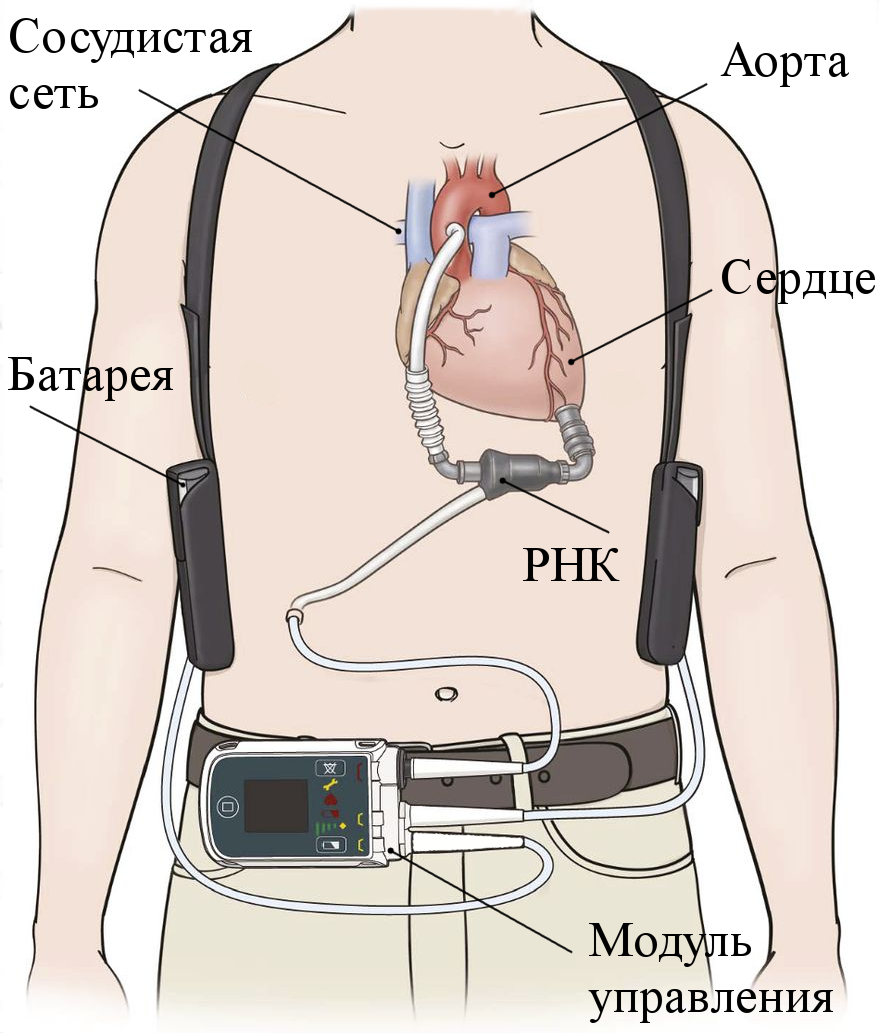
\includegraphics [scale=0.9] {../images/vad_system}}
  \end{minipage}
  \hfill
  \begin{minipage}[ht]{0.55\linewidth}
    \center{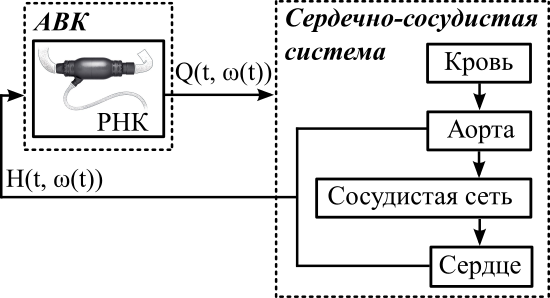
\includegraphics [scale=1.85] {../images/system_links}}
  \end{minipage}
  \caption{Представление аппарата вспомогательного кровообращения (АВК) в виде системы, образованной роторным насосом крови (РНК) и сердечно-сосудистой системой; $Q(t)$ -- расход насоса, $\omega(t)$ -- скорость вращения ротора насоса, $H(t)$ -- перепад давления в насосе, $t$ -- время}
  \label{img:system_links}  

\begin{tikzpicture}[node distance=1cm, overlay]  
\tikzstyle{arrow} = [thick,->,>=stealth]
\draw [arrow] (6.4, 6.3) |- (7.6, 6.3);
\draw [arrow] (7.4, 5.6) |- (6.2, 5.6);
\end{tikzpicture} 

\end{figure}

% В левой части рисунка \ref{img:system_links} представлена схема взаимодействия АВК и тела пациента; в правой части -- процесс взаимодействия АВК и сердечно-сосудистой системы при помощи РНК. При этом расход насоса $Q(t)$ определяется скоростью вращения ротора $\omega(t)$ и взаимосвязан с параметрами сердечно-сосудистой системы.

% При этом также возникает необходимость разработки методов и алгоритмов идентификации таких систем.

 \aim\ диссертационной работы является разработка и исследование способов структурно-параметрической идентификации имплантируемых роторных насосов крови для повышения эффективности идентификации и управления имплантируемыми роторными насосами крови в аппаратах вспомогательного кровообращения.

%разработка и исследование алгоритма идентификации для управления имплантируемым роторным насосом крови в аппаратах вспомогательного кровообращения.

% идентификация и управление имплантируемым роторным насосом крови в аппаратах вспомогательного кровообращения.
% \newpage
В~соответствии с целью диссертационной работы поставлены следующие {\tasks}:
\begin{enumerate}
  \item Разработка математической модели идентификации имплантируемого роторного насоса крови на основе расходно-напорных характеристик.
  \item Разработка математической модели сердечно-сосудистой системы с учетом имплантации роторного насоса крови.
  \item Исследование взаимодействия имплантируемого роторного насоса крови и сердечно-сосудистой системы методами математического моделирования и анализ результатов исследования с целью повышения эффективности идентификации и управления имплантируемым роторным насосом крови.
  \item Исследование взаимодействия имплантируемого роторного насоса крови и сердечно-сосудистой системы с использованием экспериментальных данных для роторных насосов крови Спутник с целью верификации результатов математического моделирования.
%   \item Разработать алгоритм идентификации имплантируемого роторного насоса крови на основе расходно-напорных характеристик, полученных в результате экспериментального исследования имплантируемых роторных насосов крови и опубликованных в литературе.
%   \item Исследовать разработанный алгоритм идентификации имплантируемого роторного насоса крови с использованием математической модели сердечно-сосудистой системы. % возможности алгоритма для управления имплантируемым роторным насосом крови с помощью моделирования взаимодействия  роторного насоса и сердечно-сосудистой системы в условиях сердечной недостаточности. % можно описать раздельно или переформулировать
%   \item Исследовать разработанный алгоритм идентификации с использованием результатов экспериментального исследования имплантируемых роторных насосов крови <<Спутник>> в испытательном гидродинамическом стенде.
%   \item Разработать способ управления имплантируемым роторным насосом крови на основе результатов исследования алгоритма идентификации. 
\end{enumerate}

% -----------------------------------------------------------------------------------------------------------------------------------
% -----------------------------------------------------------------------------------------------------------------------------------
%\newpage
\novelty
\begin{enumerate}
  % что нового в разработке, исследовании и управлении?
  \item Разработан алгоритм структурно-параметрической идентификации, который позволяет построить математическую модель в соответствии с критериями оценки эффективности идентификации для управления имплантируемыми роторными насосами крови. \\На основе построенной математической модели разработан способ управления имплантируемым роторным насосом крови, направленный на поддержание заданного уровня расхода насоса и предотвращение следующих нежелательных режимов работы насоса: обратное течение через насос, полная разгрузка желудочка сердца и коллапс желудочка сердца.
  \item Предложены следующие критерии, которые позволяют оценить эффективность идентификации для управления имплантируемыми роторными насосами крови: точность оценки расхода насоса и точность определения перехода между режимами работы насоса. \\С использованием алгоритма структурно-параметрической идентификации и в соответствии с предложенными критериями оценки эффективности идентификации построены математические модели имплантируемых роторных насосов крови Спутник.
  \item В результате комплексного исследования взаимодействия имплантируемого роторного насоса крови и сердечно-сосудистой системы на основе математической модели идентификации разработан метод определения следующих режимов работы имплантируемого роторного насоса крови: обратное течение через насос, частичная и полная разгрузка желудочка сердца, и коллапс желудочка сердца.
\end{enumerate}

% -----------------------------------------------------------------------------------------------------------------------------------
% -----------------------------------------------------------------------------------------------------------------------------------

\influence\ 
\begin{enumerate}
 \item Разработанные программные средства использованы при моделировании взаимодействия имплантируемого роторного насоса крови и сердечно-сосудистой системы и теоретическом исследовании имплантируемых роторных насосов крови Спутник. 
 \item Разработанный алгоритм структурно-параметрической идентификации может быть использован для управления имплантируемыми роторными насосами крови при проведении экспериментальных исследований в испытательных гидродинамических стендах. % напиши конкретно на ком и на чем
\end{enumerate}

% -----------------------------------------------------------------------------------------------------------------------------------
% -----------------------------------------------------------------------------------------------------------------------------------

\underline{\textbf{Личный вклад автора.}}

Автор принимал активное и непосредственное участие в выполнении всех работ, которые легли в основу диссертации.

\defpositions

\begin{enumerate}
  % с требуемой точностью % обеспечивает следующие возможности для управления: оценка расхода насоса и определение режимов работы насоса. %\vskip5pt
  %\item Разработан алгоритм идентификации, который позволяет повысить эффективность управления имплантируемым роторным насосом крови в аппаратах вспомогательного кровообращения.
 % \item Разработанный метод определения режимов работы имплантируемого роторного насоса крови позволяет определять следующие переходы между режимами работы насоса, что подтверждается результатами моделирования и исследования с использованием экспериментальных данных для роторных насосов крови Спутник: обратное течение через насос, частичная и полная разгрузка желудочка сердца, и коллапс желудочка сердца. %, что подтверждается результатами моделирования и исследования с использованием экспериментальных данных.
 \item Предложены критерии, которые позволяют оценить эффективность идентификации для управления имплантируемыми роторными насосами крови в аппаратах вспомогательного кровообращения.
  \item Разработанный алгоритм структурно-параметрической идентификации позволяет построить математические модели имплантируемых роторных насосов крови в соответствии с критериями оценки эффективности идентификации.
  \item Построенные математические модели имплантируемых роторных насосов крови позволяют определить переходы между следующими режимами работы насоса: обратное течение через насос, частичная и полная разгрузка желудочка сердца, и коллапс желудочка сердца.
  \item Разработанный способ управления имплантируемым роторным насосом крови позволяет поддерживать заданный уровень расхода насоса и предотвращать следующие нежелательные режимы работы насоса: обратное течение через насос, полная разгрузка желудочка сердца и коллапс желудочка сердца. 
 %, что позволяет повысить эффективность управления насосом в аппаратах вспомогательного кровообращения.
  %\item Разработанная модель идентификации имплантируемого роторного насоса крови позволяет описать расходно-напорные характеристики с требуемым уровнем точности. 
\end{enumerate}

% \begin{enumerate}
%   \item Разработанная математическая модель имплантируемого роторного насоса крови позволяет учесть влияние вязкости и инерции жидкости на расходно-напорные характеристики роторного насоса крови.
%   \item Разработанный метод определения режимов работы насоса позволяет с высокой точностью определить режимы работы насоса посредством анализа динамики течения жидкости через насос с помощью математической модели роторного насоса крови. %исследования на математической модели сердечно-сосудистой системы и результатами верификации с использованием данных экспериментального исследования. 
%   \item Разработанный алгоритм управления работой имплантируемого роторного насоса крови обеспечивает соответствие основным требованиям к управлению работой имплантируемого роторного насоса крови для аппаратов вспомогательного кровообращения.
%   \item Предложенный алгоритм разработки математической модели имплантируемого роторного насоса крови на основе результатов экспериментального исследования роторного насоса крови позволяет обеспечить высокую точность оценки расхода насоса и определения режимов работы насоса.
% \end{enumerate}


% -----------------------------------------------------------------------------------------------------------------------------------
% -----------------------------------------------------------------------------------------------------------------------------------

\methodology\ % Основными методами исследования в диссертационной работе являются методы математического моделирования и оптимизации. %Экспериментальное исследование выполнено \textit{in vitro} в испытательном гидродинамическом стенде. % программных библиотек
%Обоснованность результатов моделирования подтверждена данными экспериментальных исследований на гидродинамическом стенде.

% пиши конкретно: экспериментальное исследование чего? методы исследования можно отразить в задачах работы

Методами исследования диссертационной работы являются методы системного анализа и математического моделирования. 

%Обработка и анализ данных выполнены с использованием языка программирования Python.
%Идентификация имплантируемых роторных насосов крови проведена с использованием алгоритмов оптимизации Левенберга-Марквардта и дифференциальной эволюции. 

% -----------------------------------------------------------------------------------------------------------------------------------
% -----------------------------------------------------------------------------------------------------------------------------------

\reliability\ полученных результатов обусловлена корректностью поставленных задач, комплексным характером проведенных исследований и согласием полученных результатов с литературными данными. %литературными данными и результатами экспериментального исследования. 

%использованием апробированных методов моделирования
%использованием проверенных подходов к моделированию динамики кровообращения

% -----------------------------------------------------------------------------------------------------------------------------------
% -----------------------------------------------------------------------------------------------------------------------------------

\probation\
Основные результаты диссертационной работы были представлены на следующих конференциях: % докладывались

\begin{itemize}
 \item 44th Annual ESAO and 7th IFAO Congress (г. Вена, Австрия, 2017),
 \item 2nd International Symposium <<Physics, Engineering and Technologies for Biomedicine>> (г. Москва, 2017),
 \item 20-23-я всероссийская конференция <<Микроэлектроника и информатика>> (г. Москва, 2013 -- 2016),
 \item 61-62nd ASAIO Annual Conference (г. Чикаго, США, 2015; г. Сан-Франциско, США, 2016),
 \item 24th Congress of the International Society for Rotary Blood Pumps (г. Мито, Япония, 2016),
 \item X-XI German-Russian Conference on Biomedical Engineering (г. Санкт-Петербург, 2014; г. Ахен, Германия, 2015),
 \item 42th Annual ESAO Congress (г. Лёвен, Бельгия, 2015),
 \item 37th Annual International Conference of the IEEE Engineering in Medicine and Biology Society (г. Милан, Италия, 2015),
 \item 16-я научно-техническая конференция <<МедТех>> (о. Кефалония, Греция, 2014),
 \item 11-я международная конференция <<Физика и радиоэлектроника в медицине и экологии>> (г. Суздаль, 2014),
 \item 6-я Троицкая конференция <<Медицинская физика и инновации в медицине>> (г. Троицк, 2014).
\end{itemize}

\implement\
Результаты диссертационной работы получены в рамках следующих проектов и исследований:

\begin{itemize}
 \item проект Российского научного фонда № 14-39-00044 <<Разработка адаптивной системы вспомогательного кровообращения с целью персонализации лечения острой формы сердечной недостаточности>> (2014 -- 2016 гг.) по приоритетному направлению <<Проведение фундаментальных научных исследований и поисковых научных исследований вновь создаваемыми научной организацией и вузом совместными научными лабораториями>>,
 \item прикладные научные исследования в рамках ФЦП <<Исследования и разработки по приоритетным направлениям развития научно-технологического комплекса России на 2014 – 2020 годы>> по теме <<Разработка аппарата длительного механического замещения функции сердца>> (RFMEFI57814X0057) (2014 -- 2016 гг.),
 \item прикладные научные исследования и экспериментальные разработки в рамках ФЦП <<Исследования и разработки по приоритетным направлениям развития научно-технологического комплекса России на 2014 – 2020 годы>> по теме <<Миниатюризация имплантируемых насосов крови для их применения в педиатрической кардиохирургии>> (RFMEFI58115X0014) (2015 -- 2017 гг.).
\end{itemize}

Результаты работы внедрены в учебный процесс института биомедицинских систем Национального исследовательского университета <<МИЭТ>> в рамках дисциплины <<Биомедицинская инженерия искусственных органов>> для магистров, обучающихся по направлению 12.04.04 <<Биотехнические системы и технологии>>.

%Российского научного фонда и Министерства образования и науки РФ в рамках ФЦП <<Исследования и разработки по приоритетным направлениям развития научно-технологического комплекса России на 2014 – 2020 годы>>.

%Результаты диссертационной работы использованы при реализации следующих проектов кафедры биомедицинских систем Национального исследовательского университета «МИЭТ»: 

%Исследования поддержаны Министерством образования и науки РФ в рамках ФЦП <<Исследования и разработки по приоритетным направлениям развития научно-технологического комплекса России на 2014 – 2020 годы>> по теме <<Разработка аппарата длительного механического замещения функции сердца>> (RFMEFI57814X0057) на 2014 -- 2016 г. и теме <<Миниатюризация имплантируемых насосов крови для их применения в педиатрической кардиохирургии>> (RFMEFI58115X0014) на 2015 -- 2017 г., и Российским научным фондом по теме <<Разработка адаптивной системы вспомогательного кровообращения с целью персонализации лечения острой формы сердечной недостаточности>> (проект № 14-39-00044) на 2014 -- 2016 г.

%\contribution\ Автор принимал активное участие \ldots № 14.578.21.0057 (RFMEFI57814X0057)  № 14.581.21.0014 (RFMEFI58115X0014) 

% -----------------------------------------------------------------------------------------------------------------------------------
% -----------------------------------------------------------------------------------------------------------------------------------

\publications\ Результаты по теме диссертации изложены в 29 научных работах, из них 11 опубликованы в рецензируемых научных изданиях, входящих в перечень Высшей аттестационной комиссии при Министерстве образования и науки Российской Федерации и в международную реферативную базу данных Scopus, 18 -- в тезисах докладов всероссийских и международных конференций. % По теме диссертации опубликована 21 научная работа, из них 8 изданы в журналах, 
 % Характеристика работы по структуре во введении и в автореферате не отличается (ГОСТ Р 7.0.11, пункты 5.3.1 и 9.2.1), потому её загружаем из одного и того же внешнего файла, предварительно задав форму выделения некоторым параметрам

%% регистрируем счётчики в системе totcounter
\regtotcounter{totalcount@figure}
\regtotcounter{totalcount@table}       % Если поставить в преамбуле то ошибка в числе таблиц
\regtotcounter{TotPages}               % Если поставить в преамбуле то ошибка в числе страниц

\textbf{Объем и структура работы.} Диссертация состоит из~введения, четырех глав, заключения, списка литературы и~трех приложений.
%% на случай ошибок оставляю исходный кусок на месте, закомментированным
%Полный объём диссертации составляет  \ref*{TotPages}~страницу с~\totalfigures{}~рисунками и~\totaltables{}~таблицами. Список литературы содержит \total{citenum}~наименований.
%
Полный объем диссертации составляет \formbytotal{TotPages}{страниц}{у}{ы}{} 
с~\formbytotal{totalcount@figure}{рисунк}{ом}{ами}{ами}
и~\formbytotal{totalcount@table}{таблиц}{ей}{ами}{ами}. Список литературы содержит  
\formbytotal{citenum}{наименован}{ие}{ия}{ий}.
    % Введение
% --------------------------------------------------------------
\chapter{Идентификация имплантируемых роторных насосов крови в аппаратах вспомогательного кровообращения} \label{chapt1}

Цель данной главы заключается в рассмотрении истории развития имплантируемых роторных насосов крови, а также проблемы идентификации данных насосов в аппаратах вспомогательного кровообращения. 

% роторного насоса крови, а также обзоре и сравнительном анализе различных способов идентификации имплантируемым роторным насосом крови в аппаратах вспомогательного кровообращения. 

%Аппараты вспомогательного кровообращения (АВК) успешно применяются в качестве альтернативы трансплантации сердца при лечении тяжелых форм сердечной недостаточности \cite{Patel2014667,Mancini_2015,HT_LVAD_2013,Lima2015360,Schumerehv590,ottenberg_choices_2014,selzman_bridge_2015,drakos_clinical_2016}.

%\section{Идентификация имплантируемого роторного насоса крови} \label{sect_1_1}

\section{История развития имплантируемых роторных насосов крови в аппаратах вспомогательного кровообращения} \label{chapt1_history}

Сердечная недостаточность является тяжелым, прогрессирующим заболеванием, которое характеризуется неспособностью сердца перекачивать кровь в объеме, достаточном для обеспечения метаболических потребностей организма. Около восьми миллионов человек страдают от хронической сердечной недостаточности в России и около 5 миллионов -- в США, из которых ежегодно умирает около 900 тысяч в России и примерно 300 тысяч в США. Сердечная недостаточность является самой распространенной причиной госпитализации в стационары и смерти от сердечно-сосудистых заболеваний \cite{debakey2000odyssey, starling2011potential, ponikowski2014heart, wong2014epidemiological, selishchev2015ventricular}. 

Под сердечной недостаточностью наиболее часто подразумевают недостаточность левого желудочка сердца. Правожелудочковая недостаточность чаще наблюдается как вторичная по отношению к левожелудочковой недостаточности. Легкая сердечная недостаточность проявляется сниженной способностью переносить физическую нагрузку и развитием одышки во время физической активности. При более тяжелых формах пациент может фактически не иметь способности переносить физическую нагрузку и испытывать одышку в состоянии покоя. 
% 
% Если там их число ежегодно колеблется около двух тысяч, то у нас — около ста. Однако ни то, ни другое число даже близко не приближается к числу больных, которые нуждаются в таких трансплантациях. В США по этой причине каждый год умирает по 55 тысяч человек, в России — 110 тысяч. Вряд ли проблема доступности донорских сердец будет решена в обозримом будущем, поэтому нужда в системах вспомогательного кровообращения выходит на первое место.
% 
% Система вспомогательного кровообращения при всем многообразии ее разновидностей представляет собой, грубо говоря, насос, который гонит кровь, заменяя собой правый или левый желудочек сердца. Естественно, не все так просто: этот насос должен удовлетворять массе требований, важнейшие из которых — он должен работать со стопроцентной надежностью и не «портить» кровь, не разрушать ее элементы.

Сердечная недостаточность может являться результатом ухудшенной сократительной способности сердечной мышцы (систолическая недостаточность) или нарушенного наполнения сердца (диастолическая недостаточность). Оба механизма сердечной недостаточности можно описать с помощью контуров давление-объем желудочка сердца, представленных на рисунке \ref{img:pv_loops}. 

% \begin{figure}[ht] 
%   \center
%   \includegraphics [width=\textwidth] {../images/c1_pv_loops_failure}
%   \caption{} 
%   \label{img:}  
% \end{figure}

\begin{figure}[ht]
  \begin{minipage}[ht]{0.32\linewidth}
    \center{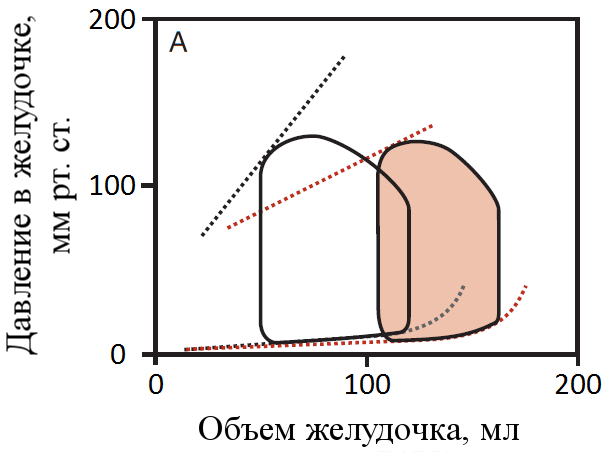
\includegraphics [scale=0.3] {../images/c1_pv_loop_systolic} \\ а)}
  \end{minipage}
  \hfill
  \begin{minipage}[ht]{0.32\linewidth}
    \center{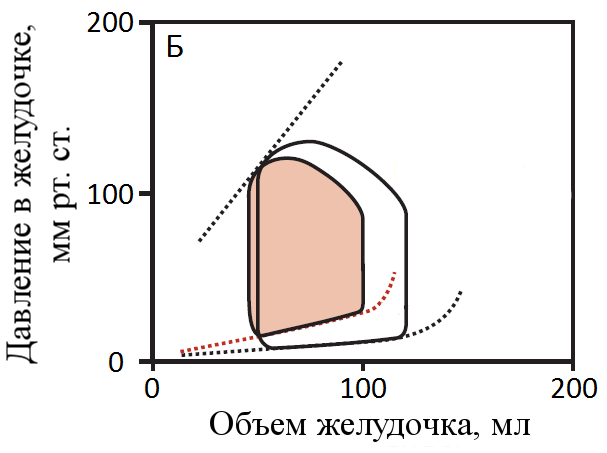
\includegraphics [scale=0.3] {../images/c1_pv_loop_diastolic} \\ б)}
  \end{minipage}
  \hfill
  \begin{minipage}[ht]{0.32\linewidth}
    \center{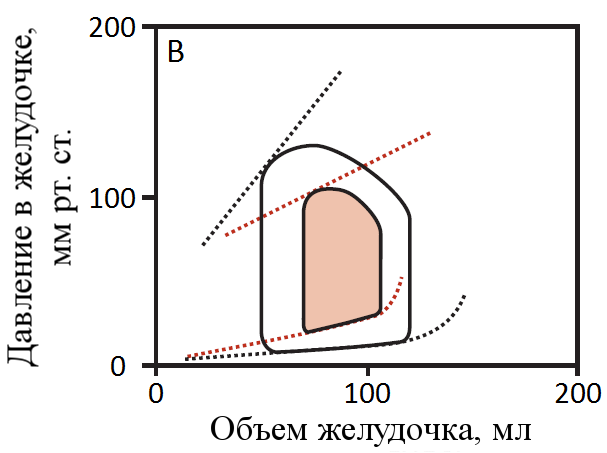
\includegraphics [scale=0.3] {../images/c1_pv_loop_comb} \\ в)}
  \end{minipage}
  \caption{Влияние систолической (а) диастолической (б) и комбинированной (в) сердечной недостаточности на контуры давление-объем желудочка сердца}
  \label{img:pv_loops}  
\end{figure}

При систолической недостаточности сердце выбрасывает меньший объем крови, что приводит к увеличению конечно-систолического объема желудочка сердца и сдвигу контура вправо -- рисунок \ref{img:pv_loops}а.

Второй тип сердечной недостаточности -- диастолическая недостаточность -- обусловлен нарушенным наполнением желудочка вследствие либо уменьшения степени растяжимости желудочка, либо нарушением релаксации. Так, снижение степени растяжимости приводит к уменьшению объема крови в желудочке и повышению диастолического давления -- контур давление-объем сдвигается влево и его площадь уменьшается. 

Хроническая сердечная недостаточность зачастую характеризуется сочетанием как систолического, так и диастолического нарушений разной степени тяжести -- рисунок \ref{img:pv_loops}в.

В настоящее время золотым стандартом лечения тяжелых форм сердечной недостаточности является трансплантация сердца. В мире ежегодно выполняется около 3500 трансплантаций, из которых примерно 2400 в США и около 100 в России \cite{frazier2017invited, transpl_ru}. Тем не менее, возможности трансплантации ограничены вследствие недостатка донорских органов и наличия целого ряда противопоказаний для пересадки. Кроме того, трансплантация требует дорогостоящей иммуносупрессивной терапии и постоянных обследований после операции. 

Альтернативной трансплантации сердца является имплантация аппаратов вспомогательного кровообращения (АВК), предназначенных для частичной или полной замены функции, как правило, левого желудочка сердца \cite{Patel2014667, Mancini_2015, HT_LVAD_2013, daners2017left}. Данный способ хирургического лечения сердечной недостаточности получил активное развитие в последние десять лет -- в настоящее время ежегодно осуществляется около 2500 имплантаций \cite{kirklin2015seventh}.

АВК могут использоваться для краткосрочной поддержки кровообращения у пациентов, ожидающих трансплантации донорского органа, для продолжительной поддержки на протяжении многих лет у пациентов, которым было отказано в трансплантации, либо для восстановления сократительной функции их собственного сердца \cite{ottenberg_choices_2014, selzman_bridge_2015, drakos_clinical_2016, wever2016cardiac}. 

Основной частью АВК является роторный насос крови (РНК), который имплантируется в грудную клетку пациента и соединяется при помощи чрескожного кабеля с системой управления.

Самые первые насосы пульсирующего типа появились в конце 70-х годов двадцатого века. Они представляли собой искусственные желудочки сердца с подвижной мембраной, обеспечивающей пульсирующий поток. В то время распространенной была гипотеза о том, что аппараты вспомогательного кровообращения должны имитировать работу биологического сердца \cite{frazier2017invited}. Среди основных насосов пульсирующего типа следует выделить, EXCOR Berlin Heart и HeartMate I, представленный на рисунке \ref{img:heartmate_one}. Аппараты вспомогательного кровообращения с насосом HeartMate I начали успешно имплантироваться с 1991 года, позволяя пациентам покинуть больницу.

\begin{figure}[ht] 
  \center
  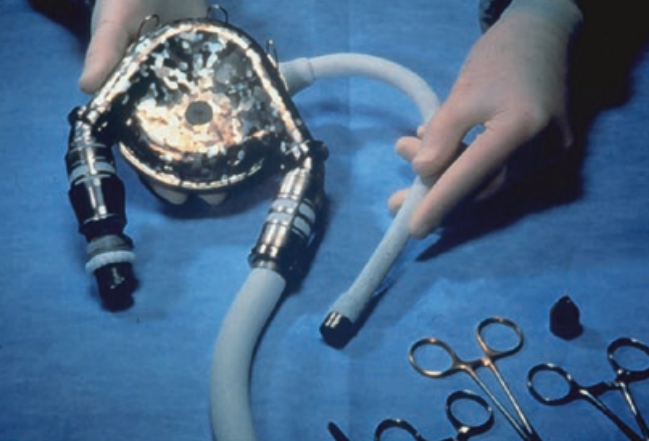
\includegraphics [width=0.6\textwidth] {../images/c1_heartmate_one}
  \caption{Насос пульсирующего типа HeartMate I \cite{frazier2017invited}} 
  \label{img:heartmate_one}  
\end{figure}

В то же время данные аппараты характеризовались невысокой надежностью по причине использования мембраны и требовали замены примерно каждые два года. Кроме того, они обладали большими размерами, не позволявшими имплантировать их женщинам и детям \cite{frazier2017invited}. 

\subsection*{Имплантируемые роторные насосы крови} \label{chapt1_irbps}

Следующим этапом развития технологии вспомогательного кровообращения стало появление роторных насосов крови \cite{reul2000blood, daners2017left}, обусловленное потребностью в продолжительной поддержке кровообращения \cite{frazier2017invited}.

Перекачивание крови в роторных насосах происходит посредством вращения рабочего колеса (ротора), создающего градиент давлений на входе и выходе насоса и обеспечивающего непрерывное течение жидкости. Ротор с постоянным магнитом внутри приводится во вращение за счет изменения магнитного поля, создаваемого статором \cite{nose1998design, mt2010n6_ru}. На входе в насос расположен направляющий аппарат (диффузор) с опорами из износостойкого материала, на выходе -- спрямляющий аппарат, в котором так же установлены опоры для ротора. Описанные компоненты образуют проточную часть насоса. Пример проточной части роторного насоса крови Спутник представлен на рисунке \ref{img:pump_view}а. Геометрия данной части насоса проектируется таким образом, чтобы добиться минимальной травмы крови с учетом высокой скорости вращения ротора насоса.

% \begin{figure}[ht] 
%   \center
%   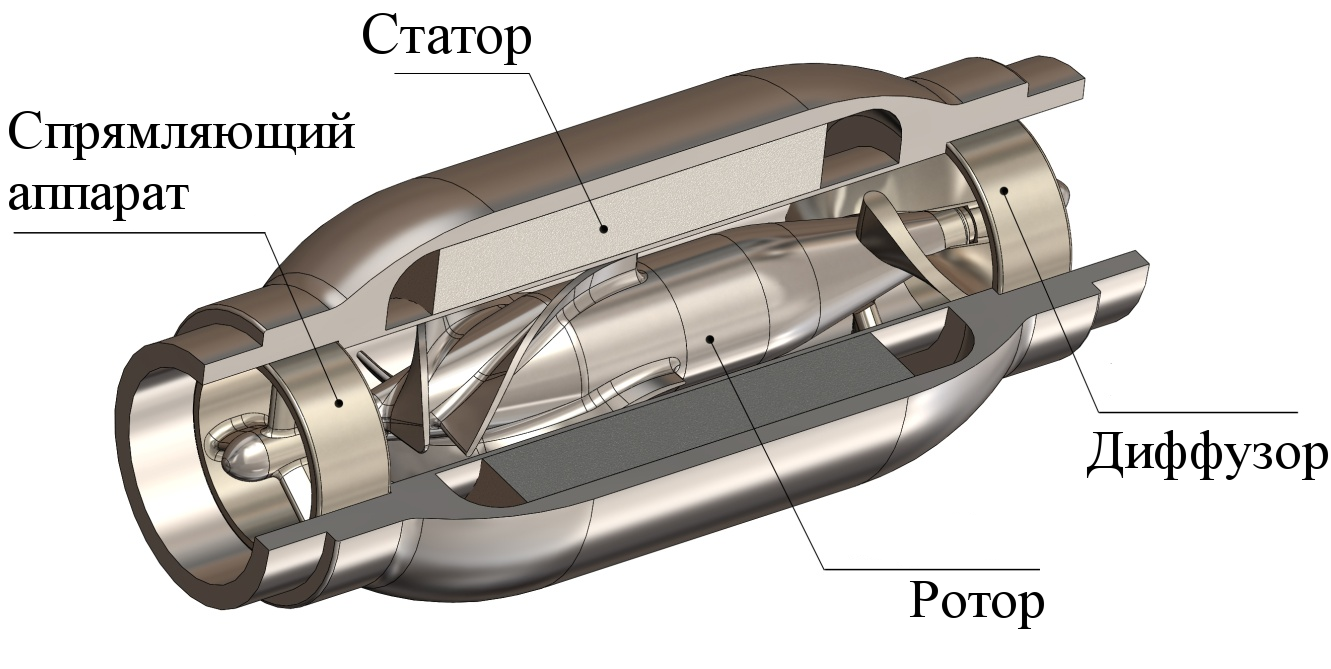
\includegraphics [width=0.6\textwidth] {../images/c1_sputnik_flow_part}
%   \caption{Проточная часть роторного насоса крови Спутник} 
%   \label{img:pump_view}  
% \end{figure}


\begin{figure}[ht]
%\fbox{
  \begin{minipage}[ht]{0.54\linewidth}
    \center{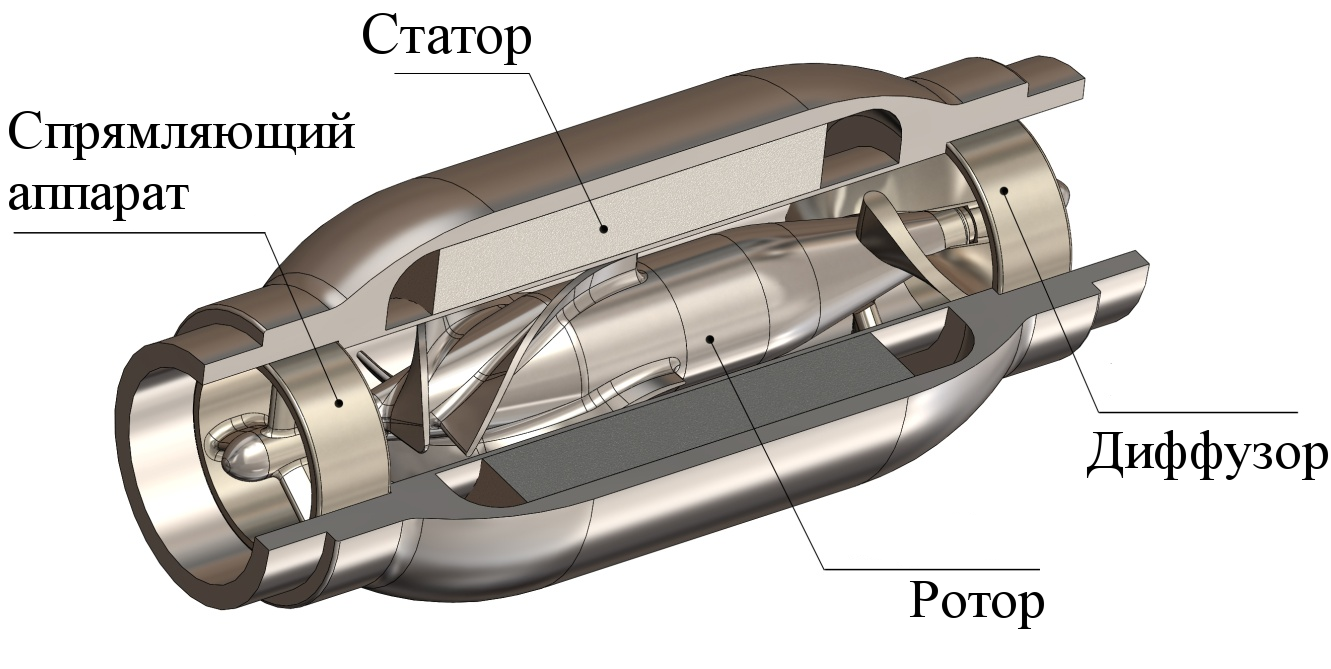
\includegraphics [scale=0.56] {../images/c1_sputnik_flow_part} \\ а)}
  \end{minipage} 
  \hfill
  \begin{minipage}[ht]{0.42\linewidth}
    \center{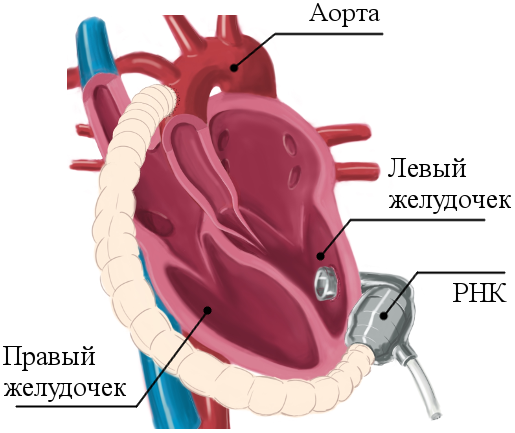
\includegraphics [scale=0.52] {../images/c1_pump_implantation_upd} \\ б)}
  \end{minipage}
  \caption{Проточная часть имплантируемого роторного насоса крови (а) и схема подключения насоса для поддержки кровообращения левого желудочка сердца (б)}
  \label{img:pump_view}  
\end{figure}

Роторные насосы крови, как правило, используются для поддержки кровообращения левого желудочка сердца. В этом случае входная канюля насоса подключается к левому желудочку сердцу, выходная -- к аорте -- рисунок \ref{img:pump_view}б. 

Первым роторным насосом, успешно применяемым в клинических условиях, стал Hemopump -- разработка Ричарда Вамплира, впервые имплантированная в 1988 году при участии доктора Фрейзера \cite{frazier2017invited}. Данный насос продемонстрировал возможность долговременной поддержки кровообращения при непульсирующем потоке крови через насос. Впоследствии на основе Hemopump был разработан роторный насос крови HeartMate II. 

В современной клинической практике представлено множество роторных насосов крови \cite{Patel2014667}. С 2000-го года имплантировано более 30 тысяч насосов, продолжительность поддержки кровообращения достигла 10 лет. Их широкое распространение обусловлено малыми массогабаритными параметрами, высокой надежностью и минимальной степенью гемолиза и тромбоэмболических осложнений. Среди наиболее известных и широко используемых роторных насосов крови следует выделить насосы Jarvik, HeartMate и HeartWare \cite{frazier2017invited, intermacs2017}. 

В результате рассмотрения исторического развития имплантируемых роторных насосов крови была подготовлена обзорная статья для журнала <<Медицинская техника>> \cite{mt6_2014}. Помимо роторных насосов крови, обеспечивающих частичную поддержку кровообращения, в современной клинической практике представлены аппараты для полной замены функции биологического сердца -- полностью искусственные сердца. Результаты обзора данных аппаратов, а также перспективы развития данной технологии были опубликованы в работах \cite{mt4_2015, mt5_2015}.

\subsubsection*{Jarvik 2000}

Разработка Jarvik 2000 началась в 1988 году при участи Jarvik Heart Inc. и Texas Heart Institute (THI). В апреле 2000 года в THI начались испытания Jarvik 2000 в качестве моста к трансплантации, а в марте 2005 был получен допуск Управления по санитарному надзору за качеством пищевых продуктов и медикаментов, мае 2005 года получен знак соответствия европейским стандартам качества (CE mark). 

Роторный насос Jarvik с осевым направлением течения, представленный на рисунке \ref{img:diff_pumps}а, имплантируется через подшиваемую манжету в левый желудочек сердца. Размеры насоса 2,5 см в ширину и 5,5 см в длину, вес -- 85 грамм. Внутри титанового корпуса насоса находится ротор, который представляет собой неодимий-ферроборовый магнит с титановыми лопатками, удерживаемый с помощью керамических подшипников. Скорость вращения ротора может изменяться от 8000 до 12000 об/мин, обеспечивая расход до 8 л/мин \cite{Westaby13101998, Healy20151794, Jarvik_cone_bearing_2013}. Одним из необходимых требований к имплантации Jarvik является площадь поверхности тела пациента не менее 1,2 м$^2$ (для сравнения нормальное значение для взрослых 1,73 м$^2$, для детей 12-13 лет -- 1,33 м$^2$).

%Система управления насосом позволяет изменять скорость вращения ротора вручную, либо автоматически с изменяемой длительностью импульсов. Комплект батарей обеспечивает до 8 часов бесперебойной работы. 

\subsubsection*{Incor}

Имплантируемый роторный насос Incor (Berlin Heart Inc., Германия) представлен на рисунке \ref{img:diff_pumps}б. 

Вес насоса составляет 200 грамм, длина -- 12 см, диаметр -- 3 см. Скорость вращения ротора насоса может изменяться от 5 до 10 тысяч об/мин, обеспечивая расход насоса до 7 л/мин. Контактирующие с кровью поверхности покрыты слоем гепарина по специальной технологии Carmeda BioActive Surface. Данный насос также обладает системой датчиков, позволяющей измерять перепад давления в насосе, что при известной скорости вращения ротора и геометрии насоса позволяет очень точно определить его расход \cite{Schmid20051188, Hetzer01062004}. 

%Система управления отображает и позволяет изменять параметры насоса. Комплект батарей обеспечивает до 12 часов бесперебойной работы.

\subsubsection*{DuraHeart}

Данный насос центробежного типа, представленный на рисунке \ref{img:diff_pumps}в, разработан компанией Terumo Heart, Inc. (США) для долговременной поддержки кровообращения. Насос состоит из двух титановых камер: в первой находятся позиционные сенсоры и ротор, во второй – бесколлекторный двигатель, который вращает ротор посредством индуктивной связи. 

Вес насоса составляет 540 грамм, диаметр -- 7,2 см, толщина -- 45 мм. Контактирующие с кровью поверхности насоса имеют гепариносодержащее покрытие. Скорость вращения ротора можно изменять в диапазоне от 1200 до 2400 об/мин, что позволяет обеспечить расход до 8 л/мин.

В настоящее время насос может имплантироваться в США в исследовательских целях \cite{DuraHeart, Morshuis01062009}.

% \begin{figure}[ht] 
%   \center
%   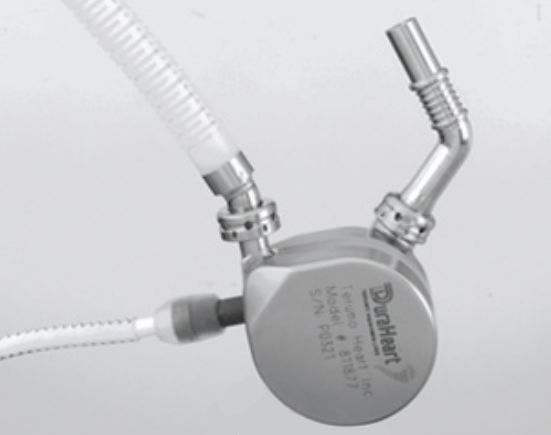
\includegraphics [width=0.6\textwidth] {../images/c1_duraheart_pump}
%   \caption{Роторный насос крови DuraHeart \cite{Morshuis01062009}} 
%   \label{img:duraheart_pump}  
% \end{figure} 

\begin{figure}[ht]
  \begin{minipage}[ht]{0.32\linewidth}
    \center{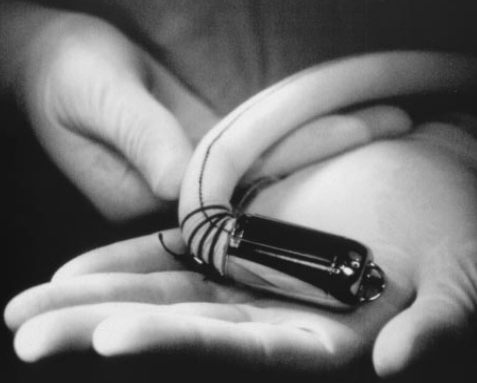
\includegraphics [scale=0.5] {../images/c1_jarvik_pump} \\ а)}
  \end{minipage}
  \hfill
  \begin{minipage}[ht]{0.32\linewidth}
    \center{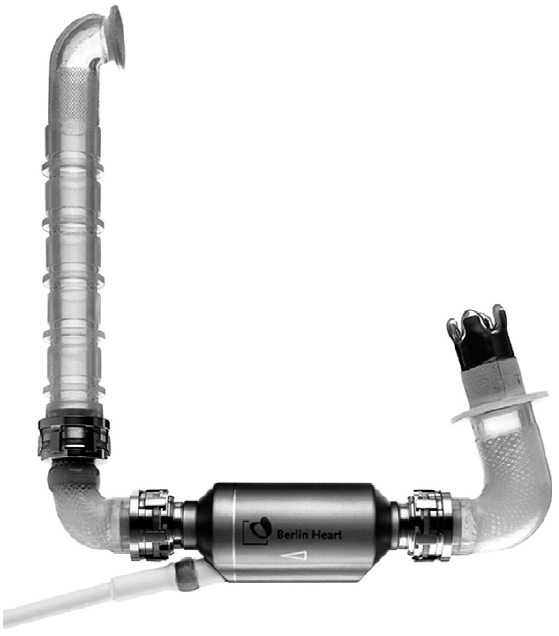
\includegraphics [scale=0.4] {../images/c1_incor_pump} \\ б)}
  \end{minipage}
  \hfill
  \begin{minipage}[ht]{0.32\linewidth}
    \center{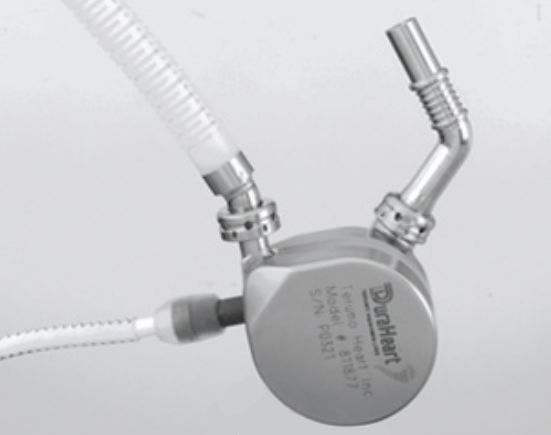
\includegraphics [scale=0.45] {../images/c1_duraheart_pump} \\ в)}
  \end{minipage}
  \caption{Роторные насосы крови Jarvik (а) \cite{Frazier2001S125}, Incor (б) \cite{Nakashima2009199} и DuraHeart (в) \cite{Morshuis01062009}}
  \label{img:diff_pumps}  
\end{figure}

\subsubsection*{ReliantHeart aVAD}

Разработка данного насоса началась в 1988 году при участи доктора Дебейки, инженеров из NASA и Бейлорского медицинского колледжа. В ноябре 1998 года в Берлине проведена первая имплантация. В апреле 2001 получен знак соответствия европейским стандартам качества, в феврале 2004 получен допуск Управления по санитарному надзору за качеством пищевых продуктов и медикаментов.

Обновленная версия насоса под названием HeartAssist5 \cite{HeartAssistFlow} получила знак соответствия европейским стандартам в мае 2009 года. В настоящее время данный роторный насос известен под названием ReliantHeart aVAD.

Роторный насос aVAD (ReliantHeart Inc., США) с осевым направлением течения позволяет обеспечить расход до 6 л/мин. Ротор насоса содержит шесть лезвий и вращается со скоростью 7500-12500 об/мин. Диаметр насоса -- 38 мм, длина -- 71 мм, вес -- 92 грамм. aVAD является единственным насосом, обладающим датчиком расхода на выходной канюле. Энергопотребление насоса составляет 10 Вт, продолжительность работы от батарей до 10 часов \cite{Loforte2017}. 

% \begin{figure}[ht] 
%   \center
%   \includegraphics [width=0.6\textwidth] {../images/c1_avad_pump}
%   \caption{Роторный насос крови ReliantHeart aVAD} 
%   \label{img:avad_pump}  
% \end{figure}

%Таким образом, суммарное время работы системы без подзаряда батарей составляет 5-8 часов. Система управления обладает функциональным набором, схожим с системой HeartWare.

\subsubsection*{HeartMate}

Наиболее часто имплантируемым роторным насосом с осевым направлением течения является HeartMate II (Thoratec Corp., США), представленный на рисунке \ref{img:heartmate_pumps}а. С момента выхода этой системы со стадии клинических испытаний в начале 2000-х годов по всему миру было имплантировано более 10 тысяч таких насосов \cite{frazier2017invited}.

\begin{figure}[ht]
  \begin{minipage}[ht]{0.48\linewidth}
    \center{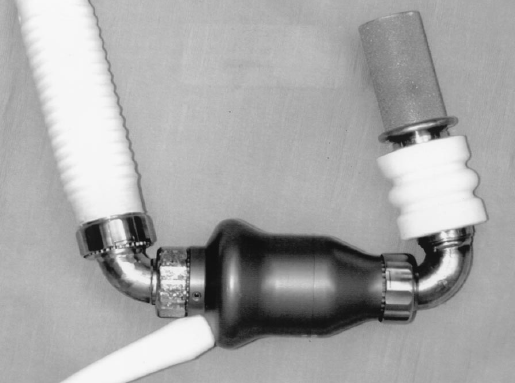
\includegraphics [scale=0.65] {../images/c1_heartmate_2_pump} \\ а)}
  \end{minipage}
  \hfill
  \begin{minipage}[ht]{0.48\linewidth}
    \center{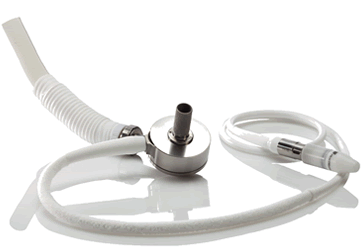
\includegraphics [scale=0.60] {../images/c1_heartmate_3_pump} \\ б)}
  \end{minipage}
  \caption{Роторные насосы крови HeartMate II (а) \cite{Griffith_2001} и HeartMate III (б) \cite{molina2013current}}
  \label{img:heartmate_pumps}  
\end{figure}

В ноябре 2005 года насос получил знак соответствия европейским стандартам качества, в апреле 2008 года -- допуск Управления по санитарному надзору за качеством пищевых продуктов и медикаментов \cite{HeartMate_II_Sheikh}. 

Вес насоса составляет 350 грамм, диаметр около 4 см и длина -- 7 см. Внутри насоса находится ротор, вращающийся посредством электродвижущей силы, генерируемой мотором. Скорость насоса может изменяться от 6000 об/мин до 15000 об/мин, обеспечивая поток крови до 10 л/мин \cite{Loforte20091357}. Время бесперебойной работы от аккумуляторов составляет около четырех часов \cite{Griffith_2001}. 

Обновленная версия насоса разработана компаниями Thoratec Corporation Inc. и Levitronix GmbH, называется HeartMate III (рисунок \ref{img:heartmate_pumps}б). Размеры насоса составляют 6,9 см в диаметре и 3 см в толщину, вес -- 500 грамм \cite{farrar2007design}. Ключевой особенностью данного насоса являются текстурированная внутренняя поверхность, уменьшающая требования к использованию антикоагулянтов, а также режим создания искусственных пульсаций потока и возможность косвенной оценки расхода с использованием собственных параметров насоса \cite{heartmate_speed_modulations, Schumerehv590}. Предполагается, что искусственные пульсации уменьшают не только вероятность образования тромбов, но и энергопотребление насоса. 

\subsubsection*{HeartWare}

Компания HeartWare Inc. (США) выпускает два роторных насоса крови центробежного типа -- HVAD и MVAD, представленных на рисунке \ref{img:heartware_pumps} \cite{larose2010design, cheung2015design}.
 
\begin{figure}[ht]
  \begin{minipage}[ht]{0.48\linewidth}
    \center{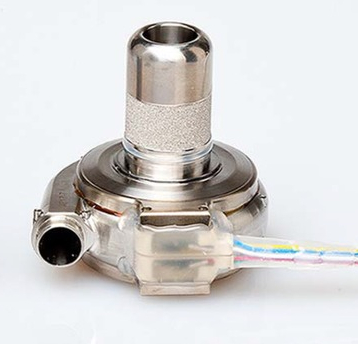
\includegraphics [scale=1.2] {../images/c1_hvad_pump} \\ а)}
  \end{minipage}
  \hfill
  \begin{minipage}[ht]{0.48\linewidth}
    \center{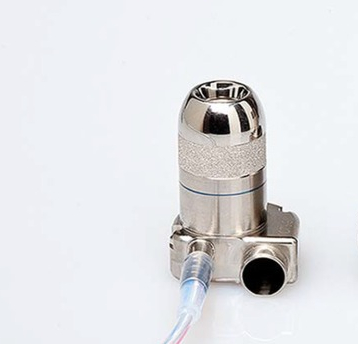
\includegraphics [scale=1.2] {../images/c1_mvad_pump} \\ б)}
  \end{minipage}
  \caption{Роторные насосы крови HVAD (а) и MVAD (б) \cite{cheung2015design}}
  \label{img:heartware_pumps}  
\end{figure}

На сегодняшний день HVAD является одним из наиболее широко используемых роторных насосов центробежного типа \cite{chorpenning2014heartware, rich2017hvad}. В январе 2009 года данный насос получил знак соответствия европейским стандартам (CE mark), в ноябре 2011 был получен допуск Управления по санитарному надзору за качеством пищевых продуктов и медикаментов для использования HVAD в качестве моста к трансплантации \cite{Carrel01012013}. 

Входная канюля данного насоса вставляется в левый желудочек сердца аналогично насосу Jarvik. В HVAD используются магнитные и гидродинамические опоры рабочего колеса, благодаря чему оно не изнашивается в процессе работы. Рекомендованная скорость вращения ротора данного насоса изменяется в пределах от 2400 до 3200 об/мин, обеспечивая расход 3,5-8 л/мин при энергопотреблении от 2,5 до 8,5 Вт, вес насоса составляет 160 грамм.

Роторный насос крови MVAD характеризуется меньшими размерами и весом (78 грамм). Скорость вращения ротора изменяется в пределах от 8 до 18 тысяч об/мин, обеспечивая расход до 7 л/мин. В настоящее время MVAD находится на этапе клинических испытаний \cite{cheung2015design}.

\subsubsection*{Спутник}

В настоящее время роторный насос крови Спутник, представленный на рисунке \ref{img:sputnik_pumps}а, успешно применяется в клинических условиях \cite{selishchev2015ventricular}. Имеет осевое направление течения, диаметр насоса составляет 35 мм, длина -- 82 мм, вес - 246 грамм, энергопотребление -- 8 Вт, скорость вращения ротора может изменяться от 5 до 10 тысяч об/мин.

\begin{figure}[ht]
  \begin{minipage}[ht]{0.48\linewidth}
    \center{\includegraphics [scale=0.235] {../images/c1_s1} \\ а)}
  \end{minipage}
  \hfill
  \begin{minipage}[ht]{0.48\linewidth}
    \center{\includegraphics [scale=0.235] {../images/c1_s2} \\ б)}
  \end{minipage}
  \caption{Имплантируемые роторные насосы крови Спутник первого (а) и второго поколений (б)}
  \label{img:sputnik_pumps}  
\end{figure}

Насос первого поколения был имплантирован 9 июня 2012 года 67-летнему пациенту с последующей успешной трансплантацией сердца. На сегодняшний день произведено более тридцати имплантаций насоса.

Помимо этого разрабатывается улучшенная версия насоса -- Спутник 2, представленная на рисунке \ref{img:sputnik_pumps}б. В данной версии диаметр был уменьшен до 29 мм, длина -- до 66 мм, энергопотребление было уменьшено на 15\%, масса -- до 205 грамм \cite{sputnik_upd}. В настоящее время проводятся испытания насоса на животных.

%Отмечается, что АВК Спутник в 2 раза дешевле заграничных аналогов, при этом он не уступает им в качестве и надежности \cite{lvad_ru}.

\section{Сравнительный анализ способов идентификации имплантируемых роторных насосов крови}\label{identification_review}

Таким образом, в современной клинической практике существует огромный выбор имплантируемых роторных насосов крови.

В то же время данные насосы пассивно реагируют на изменение состояния сердечно-сосудистой системы, что может приводить к коллапсу желудочка сердца, аритмии, отеку легких и внутренним кровотечениям \cite{tchantchaleishvili2017clinical, bozkurt2015physiologic,giridharan_hemodynamic_2015,mahr_intermittent_9000, aggarwal_incidence_2012, wever_pulsatility_2013, vollkron_suction_2007,salamonsen_anatomy_2015}. Это создает существенные риски для пациента и ограничивает безопасность и производительность АВК. Кроме того, высокая рабочая скорость насоса может приводить к коллапсу желудочка сердца, а также увеличению вероятности гемолиза и тромбообразования \cite{Vollkron2006, vollkron_suction_2007,Ng_2013}. В то же время, малая скорость насоса может приводить к обратному течению через насос \cite{giridharan_hemodynamic_2015, bozkurt2015physiologic}. 

Одним из основных направлений развития технологии вспомогательного кровообращения является управление имплантируемым роторным насосом крови, направленное на преодоление указанных проблем и повышение эффективности лечения различных форм сердечной недостаточности \cite{schima_noninvasive_1992,schloglhofer_international,JTD2878,Kyo2012101,lenneman2014treatment,Controller_review}.

На основе проведенного обзора алгоритмов управления имплантируемым роторным насосом крови была подготовлена и опубликована статья в журнале <<Медицинская техника>> \cite{mt3_2016}.

Для управления имплантируемыми роторными насосами крови необходима идентификация, которая понимается как построение математической модели системы по результатам экспериментальных исследований \cite{identification_usa}. 

% На данный момент предложено множество различных способов управления имплантируемым роторным насосом крови \cite{bozkurt2015physiologic,walter2012control,Controller_review,amacher2014synchronized,tchantchaleishvili2017clinical, moscato2010left}. Так, в работе S. Bozkurt \cite{bozkurt2015physiologic} описывается алгоритмы управления скоростью вращения ротора насоса, в том числе посредством задания профилей скорости. В работе M. Walter и др. \cite{walter2012control} рассматриваются общие принципы управления в биомедицинских применениях применительно к имплантируемым РНК. Наиболее полный обзор различных способов управления РНК представлен в работе AlOmari и др. \cite{Controller_review}. 

%Таким образом, на сегодняшний день разработано множество роторных насосов крови для управления которыми необходима идентификация. 

Обзор различных способов идентификации имплантируемого роторного насоса крови представлен в работах C. Bertram и A. AlOmari \cite{bertram2005measurement, Controller_review}. Построенные в результате идентификации математические модели используются при управлении системой и предсказания поведения идентифицируемой системы в будущем \cite{identification_usa}. 

В случае с роторными насоса крови построенные в результате идентификации математические модели могуть быть использованы для оценки физиологических параметров в сердечно-сосудистой системе с имплантированным насосом -- таких как,  перепад давления в насосе, давление в аорте, расход насоса и т.\:д. Полученные качественные и количественные данные о взаимодействии насоса и сердечно-сосудистой системы могут быть использованы для управления имплантируемым РНК. 

Так в системе управления HeartWare HVAD используется алгоритм оценки расхода насоса на основе таблиц о соотношении энергопотребления и расхода насоса, которые получены в результате экспериментального исследования насоса в испытательном гидродинамическом стенде \cite{reyes2016accuracy}. 

В работе F. Moscato и др. по идентификации разработана математическая модель на основе результатов экспериментального исследования РНК Micromed DeBakey \cite{Moscato_2009}. Разработанная модель описывается следующим уравнением:

\begin{equation}
	H(t) = \alpha \omega(t)^2 - \left[ aQ(t) + bQ(t)^2 \right] - L\frac{dQ(t)}{dt},
	\label{eq:moscato_equation}
\end{equation}

\noindent где $H(t)$ -- перепад давления в насосе, $\omega(t)$ -- скорость вращения ротора насоса, $Q(t)$ -- расход насоса, $\alpha$ -- параметр, связанный со скоростью вращения ротора, $a$ и $b$ -- параметры, характеризующие гидравлическое сопротивление, $L$ -- параметр, характеризующий инерцию жидкости в насосе. В работе продемонстрировано влияние инерции жидкости на расходно-напорную характеристику насоса, сделаны выводы о необходимости включения члена $LdQ/dt$ в уравнение, что позволяет улучшить точность оценки расхода насоса в пульсирующих условиях.

В работах T. Pirbodaghi предлагаются математические модели, разработанные на основе результатов исследований в испытательном гидродинамическом стенде \cite{Pirbodaghi_2011, Pirbodaghi_2017}. Пример математической модели согласно \cite{Pirbodaghi_2017} приводится далее: 

\begin{equation}
	H(t) = b_0Q(t) + b_1Q(t)^2 + b_2\omega(t)^2 + b_3\frac{dQ(t)}{dt} + b_4\frac{d\omega(t)}{dt},
	\label{eq:pirbodaghi_equation}
\end{equation}

\noindent где $H(t)$ -- перепад давления в насосе, $Q(t)$ -- расход насоса, $\omega(t)$ -- скорость вращения ротора насоса, $t$ -- время, $b_i$ -- коэффициенты уравнения. Указано, что добавление производных по времени позволяет увеличить точность описания работы насоса в пульсирующих условиях. 

В работе M. Granegger и др. разработана математическая модель с целью оценки расхода центробежного насоса на основе результатов исследования в гидродинамическом стенде при различных величинах вязкости жидкости \cite{Granegger_2012}. Модель описывается следующим уравнением:

\begin{equation}
	Q = aI + bI^2 + cI^3 + d\omega + e\omega^2 + g\omega I + h\omega^2 I + k - m\frac{d\omega}{dt},
	\label{eq:granegger_equation}
\end{equation}

\noindent где $Q$ -- расход насоса (л/мин), $I$ -- электрический ток (А), $\omega$ -- скорость насоса (об/мин), $a-m$ -- коэффициенты, заданные линейной функцией вида $x(\mu) = x_1\mu + x_2$, где $\mu$ -- вязкость жидкости (мПа$\cdot$с). Разработанная математическая модель характеризуется средней ошибкой при оценке расхода равной 0,06$\pm$0,31 л/мин и может быть использована для оценки сократительной способности желудочка сердца. 

В работе Г. Иткина разработаны математические модели на основе результатов исследований в испытательном гидродинамическом стенде \cite{vest_2015}. Разработанные математические модели предназначены для оценки расхода и перепада давления в насосе. Так, среднее значение расхода насоса рассчитывается согласно следующей формуле:

\begin{eqnarray}
	F_{PUMP} = K_1 + K_2\omega_{MEAN} + K_3\omega_{MEAN}^2 + K_4I_{MEAN} + K_5I_{MEAN}^2 + \nonumber \\ + K_6I_{MEAN}^3,
	\label{eq:itkin_equation}
\end{eqnarray}

\noindent где $F_{PUMP}$ -- среднее значение расхода насоса, $\omega_{MEAN}$ -- среднее значение скорости вращения ротора, $I_{MEAN}$ -- среднее значение электрического тока двигателя насоса, $K_1$, $K_2$, $K_3$, $K_4$, $K_5$ и $K_6$ -- коэффициенты. 

Также с целью оценки расхода насоса в работе E. Lim разработана математическая модель насоса, описываемая следующим уравнением \cite{Lim_2011}:

\begin{eqnarray}
	Q_p(k\tau) = 0,2710f([k-1]\tau) - 0,2546f([k-2]\tau) - 1,985Q_p([k-1]\tau) - \nonumber \\ - 1,240Q_p([k-2]\tau) - 0,2397Q_p([k-3]\tau) + e_1(k\tau),
	\label{eq:dynamic_model_lim}
\end{eqnarray}

\noindent где $Q_p$ -- расход насоса, $\tau$ -- интервал измерения равный 0,02 с, $e_1(k\tau)$ -- погрешность, $f$ -- функция, которая описывается следующим выражением:

\begin{equation}
	f = a_1 + a_2P + a_3P^2 + a_4P^3 + a_5\omega + a_6\omega^2,
\end{equation}

\noindent где $P$ -- потребляемая мощность, $a_1 - a_6$ -- коэффициенты, величина которых зависит от вязкости крови. Разработанная модель предназначена для использования в алгоритме управления расходом имплантируемого роторного насоса крови \cite{Lim_2011}. 

В работах Y. Wang и др. предлагаются математические модели насосов, предназначенные для управления расходом насосов \cite{wang2015rotary, wang2015suction}. Математические модели описываются следующими уравнениями:

\begin{equation}
	\frac{dF_p}{dt} = \frac{b_0}{b_1}F_p - \frac{b_2}{b_1}\omega^2 + \frac{1}{b_1}\Delta P,
	\label{eq:wang_equation_1}
\end{equation}

\begin{equation}
	J\frac{d\omega}{dt} = \frac{3}{2}K_BI - B\omega - a_0\omega^3 - a_1F_p\omega^2,
	\label{eq:wang_equation_1_speed}
\end{equation}

\noindent где $F_p$ -- расход насоса, $\omega$ -- скорость вращения ротора насоса, $\Delta P$ -- перепад давления в насосе, $J$ -- инерция ротора, $K_B$ -- постоянная противо-ЭДС, $I$ -- амплитуда фазового тока, $a_0$, $a_1$, $b_0$, $b_1$ и $b_2$ -- постоянные, определяемые экспериментально.

\begin{equation}
	\phi\frac{dF_p}{dt} = K_2\omega^2 - \Delta P - c_1\omega F_p - c_2\omega F_{p}^{2},
	\label{eq:wang_equation_2}
\end{equation}

\begin{equation}
	J\frac{d\omega}{dt} = K_1I - c_3\omega - c_4\omega F_p - T_R \frac{\omega}{\omega_{full}},
	\label{eq:wang_equation_2_speed}
\end{equation}

\noindent где $F_p$, $\omega$, $\Delta P$ и $J$ -- определены выше, $\phi$ -- параметр, характеризующий инерционные эффекты в насосе, $K_1$ -- коэффициент момента двигателя постоянного тока, $I$ -- электрический ток двигателя, $T_R$ -- коэффициент кинетического трения, $\omega_{full}$ -- скорость вращения ротора при полной разгрузке желудочка сердца, $K_2$, $c_1$, $c_2$, $c_3$ и $c_4$ -- параметры, зависящие от вязкости жидкости. 

Разработанные математические модели насосов исследованы на модели сердечно-сосудистой системы, продемонстрировав возможности поддержания физиологического расхода и предотвращения коллапса желудочка сердца.

В работе \cite{pennings2015estimation} разработана математическая модель по результатам исследований имплантируемых роторных насосов крови Micromed DeBakey и HeartMate II в испытательном стенде. Разработанная математическая модель предназначена для оценки давления в левом желудочке сердца и описывается следующим выражением:

\begin{eqnarray}
	P_{lv} = P_{ao} + dP_{out} - dP_{VAD},
	\label{eq:lv_pressure_estimation_pennings}
\end{eqnarray}

\noindent где $dP_{out}$ -- среднее аортальное давление, $dP_{VAD}$ -- средний перепад давления в насосе, рассчитываемый согласно следующей формуле:

\begin{equation}
	dP_{VAD}(t) = b_1Q_{VAD}(t) + b_2Q_{VAD}^{2}(t) + b_3n^2 + b_4\frac{dQ_{VAD}(t)}{dt} + dP_{hydro},
\end{equation}

\noindent где $b_1$, $b_2$, $b_3$ и $b_4$ -- коэффициенты, $Q_{VAD}$ -- расход насоса, $n$ -- скорость вращения ротора, $dP_{hydro}$ -- поправочный коэффициент, введенный из-за разницы в высоте датчиков давления левого желудочка сердца и давления на выходе насоса.

В работе \cite{hijikata2015estimating} разработана математическая модель центробежного насоса крови, предназначенная для оценки расхода насоса. Модель описывается следующим выражением:  

\begin{equation}
	Q = a'\frac{T}{n} + (b_1\mu + b_0)n + c_1\mu + c_0,
	\label{eq:hijikata_equation}
\end{equation}

\noindent где $T$ -- крутящий момент двигателя, $a'$, $b_0$, $b_1$, $c_0$ и $c_1$ -- коэффициенты, определенные экспериментально в испытательном гидродинамическом стенде,  $n$ -- скорость вращения ротора и $\mu$ -- вязкость рабочей жидкости. В ходе исследований в стенде с использованием воды абсолютная ошибка при оценке расхода не превысила 0,51 л/мин в диапазоне расхода насоса от 0 до 10 л/мин. В ходе исследований в стенде с использованием вязкой жидкости абсолютная ошибка составила менее 0,77 л/мин в аналогичном диапазоне расхода насоса.

% добавить критику работ, сделанных до меня (не приводятся алгоритмы идентификации, рассматриваются только результаты идентификации или возможности управления, которые реализованы в ходе решения задачи идентификации -- в иных условиях подход к управлению на основе данного подхода может не работать, только задача идентификации решена локально, а идентифицированная система не исследована в широком диапазоне)
% таблицы HVAD тоже идентификация, но без разработки математической модели, работа Salamonsen о преднагрузке тоже простая идентификация на основе подбора полинома, но без управления; Moscato -- нет алгоритма, добавление членов произвольно

Примеры различных математических моделей имплантируемых роторных насосов крови можно найти в работах \cite{bioengineering1010022, Moscato_2009, moscato2012evaluation, Pirbodaghi_2011, Pennings_2013, wang2015rotary, wang2015suction, alomari2011non, alomari2009non, gao2012pulsatile, Bakouri_2014, wu2009adaptive, Malagutti_2007, 4352467, Giridharan2003, simaan2009dynamical, choi2007hemodynamic, lim2008noninvasive, yoshizawa2002sensorless, kitamura2000physical, xu2000computer, takami1997flow, ayre2000sensorless}. %(не описывают как было разработано),

Следует отметить, что общим недостатком рассмотренных способов построения математических моделей имплантируемых роторных насосов крови является отсутствие универсального и общепринятого алгоритма. На построение математической модели оказывает влияние геометрия ротора насоса \cite{ayre2000sensorless}, таким образом разнообразие конструкций роторных насосов крови создает потребность в разработке универсального алгоритма идентификации. При идентификации также необходимо учитывать взаимодействие насосов с сердечно-сосудистой системой. 

% ----------------------------------------------------------------------------------------------------------------------------------------------------------------------------------------------------------------------------
% ----------------------------------------------------------------------------------------------------------------------------------------------------------------------------------------------------------------------------

%Отличие данной работы заключается в рассмотрении систем управления аппаратами вспомогательного кровообращения, которые находят применение в современной клинической практике \cite{Mancini_2015,Patel2014667}. При их рассмотрении использовались как результаты обзора патентов соответствующих компаний \cite{brown2015methods,larose2005sensorless, tamez2014vad, yomtov2015physiologically, bourque2015generating, yanai2014backflow, medvedev2016method}, так и данные, опубликованные в литературе \cite{reyes2016accuracy, chorpenning2014heartware, cheung2015design, Healy20151794, Slaughter2010S1, lund2012derived, HeartAssistFlow}. Основное внимание уделено обзору систем, методов и алгоритмов управления, опубликованных в литературе за последние пять лет. 

%Исходно предлагается следующая классификация: методы и алгоритмы оценки и регулирования расхода насоса, определения и управления режимами работы роторного насоса крови, и физиологического управления. К первым относятся методы и алгоритмы оценки расхода насоса \cite{hijikata2015estimating, Granegger_2012,vest_2015} и его регулирования с определенными целями \cite{Bozkurt20141288, Lim_2011}. Ко вторым относятся методы и алгоритмы определения состояния коллапса желудочка сердца \cite{Ng_2013, Ochsner_2013, 6359938}, состояния аортального клапана \cite{Jansen_Park01092014,Granegger_2014,Hui_2014,6944257,Hayward_2015,7295582,Ooi_2015,6862467,vest_2014} и управления данными состояниями. К третьим -- методы и алгоритмы физиологического управления, регулирующие работу насоса относительно некоторых физиологических параметров \cite{wang2015rotary, huang2014pulse,bioengineering1010022}, либо имитирующие механизм Старлинга \cite{6606105,6609590,Bakouri_2014,Salamonsen_2012,Mansouri_2015,Ochsner_2014}.

%\subsection*{Управление с постоянной скоростью насоса}

% Данный способ управления заключается в поддержании скорости вращения ротора насоса независимо от состояния сердечно-сосудистой системы либо регулировании скорости врачами в клинических условиях. В то же время, он характеризуется ограниченными возможностями для адаптации к потребностям сердечно-сосудистой системы \cite{Lim_2011, tchantchaleishvili2017clinical}. Так, роторные насосы крови уменьшают напор с увеличением расхода при постоянной скорости вращения ротора, в то время как физиологические потребности тела заключаются в увеличении расхода с увеличением давления. 

% Несмотря на это, система управления HeartAssist 5 (ReliantHeart Inc., США) позволяет поддерживать постоянную скорость вращения ротора насоса. Решение об изменении скорости вращения ротора принимается лечащим врачом на основе данных об измеренном расходе насоса, потребляемой мощности и скорости вращения ротора за последние 30 дней, которые доступны дистанционно на VADLink.com \cite{HeartAssistFlow}. 

% Описанные способы управления имплантируемыми роторными насосами крови требуют периодического посещения больницы и принятия решения лечащим врачом о регулировании скорости насоса. В то же время, система управления Jarvik 2000 (Jarvik Heart Inc., США) позволяет пациенту самостоятельно регулировать скорость вращения ротора насоса \cite{Healy20151794}. В зависимости от своего самочувствия или уровня физической активности пациент может выбирать значения в диапазоне от 1 до 5, что соответствует изменению скорости вращения ротора от 8000 об/мин до 12000 об/мин и может значительно изменять расход насоса. Предполагается, что постепенное уменьшение скорости должно обеспечить поступательное увеличение нагрузки на желудочек сердца и помочь восстановлению сердечной мышцы \cite{Healy20151794}. 

% Кроме того, в Jarvik 2000 применяется алгоритм, который уменьшает скорость вращения ротора до 7000$\pm$200 об/мин в течение 10 секунд каждую минуту. Предполагается, что это позволит уменьшить степень разгрузки левого желудочка сердца и увеличит вероятность выброса крови через аортальный клапан \cite{Jarvik_cone_bearing_2013, arndt_fully_2010}. Аналогичные алгоритмы управления разработаны для роторных насосов крови Incor (Berlin Heart GmbH, Германия) \cite{arndt_fully_2010} и HeartWare MVAD \cite{Kapur2013S53, cheung2015design}. Так, в MVAD применяется алгоритм  <<qPulse Cycle>>, который уменьшает скорость вращения ротора на 15\% или 20\% в течение 5 секунд с последующим увеличением скорости до исходного значения в течение 10-30 секунд. 
% 
% Следует отметить, что данный тип управления является общепринятым для имплантируемых роторных насосов крови, применяемых в клинической практике \cite{larose2010design, Slaughter2010S1, HeartAssistFlow, Healy20151794, advanced_development_2011,bozkurt2015physiologic}.

%\subsection*{Управление с переменной скоростью насоса}

% Данный тип управления имплантируемым роторным насосом крови позволяет автоматически по определенным правилам изменять скорость вращения ротора насоса. 

% Так, в патенте \cite{larose2005sensorless} описывается механизм управления скоростью вращения ротора, позволяющий поддерживать заданную величину расхода насоса. В работе E. Lim и др. \cite{Lim_2011} также предлагается алгоритм поддержания расхода насоса на заданном уровне. Аналогичный алгоритм управления расходом роторного насоса крови с возможностью предотвращения коллапса желудочка сердца представлен в работе \cite{simaan2009dynamical}.

% В роторном насосе крови HeartWare HVAD имеется возможность регулирования скорости вращения ротора насоса в случае обнаружения коллапса желудочка сердца \cite{brown2015methods, reyes2016accuracy, medvedev2016method}. В системе управления HeartWare MVAD также имеется алгоритм управления, реагирующий на возникновение коллапса желудочка сердца \cite{cheung2015design}. Данный алгоритм уменьшает скорость вращения ротора на 15\% с последующим увеличением до исходного значения. Если состояние коллапса не обнаруживается, то алгоритм выключается, в ином случае скорость вращения ротора уменьшается на 25\% с последующим увеличением до исходного значения. Описанный цикл повторяется до тех пор, пока состояние коллапса сохраняется.

% Подобные алгоритмы разработаны для роторных насосов крови VentrAssist \cite{mason2008reliable}, HeartMate II и Incor. Так, управление Incor заключается в поддержании заданной величины индекса пульсаций \cite{arndt_fully_2010}. Индекс пульсаций вычисляется на основе измеренного перепада давления в насосе и предназначен для предотвращения коллапса желудочка сердца.  

% %%% -----------------------------------------------------------------------------
% 
% В работе F. Moscato и др. предложен алгоритм управления скоростью роторного насоса крови на основе данных о давлении в левом желудочке сердца \cite{moscato2010left}. Давление в желудочке оценивается с помощью фильтра Калмана с увеличенной памятью и данных об аортальном давлении, расходе насоса и скорости вращения ротора. Предоженный алгоритм позволяет поддерживать определенный уровень нагрузки на желудочек сердца в различных физиологических условиях, что подтверждается исследованием на математической модели сердечно-сосудистой системы.

%%% -----------------------------------------------------------------------------

% В работе \cite{wang2015suction} предложен алгоритм управления скоростью вращения ротора насоса крови за счет поддержания фиксированной разности давления между левым желудочком и аортой. Предложенный алгоритм направлен на обеспечение физиологического расхода насоса и позволяет предотвратить коллапс желудочка сердца, что подтверждается результатами исследования на математической модели сердечно-сосудистой системы. Подобные алгоритмы управления с целью поддержания фиксированного перепада давления в насосе были предложены в работах \cite{waters1999, giridharan2002, giridharan2006}.
% 
% В работах \cite{Salamonsen_2012, Bakouri_2014} предлагается алгоритм управления скоростью вращения ротора на основе данных о величине пульсаций расхода насоса. Предлагаемый алгоритм позволяет установить равновесие между сердечным выбросом правого желудочка сердца и объединенным расходом левого желудочка и насоса, что позволяет предотвратить недостаточную и избыточную откачку крови из левого желудочка сердца. Аналогичные алгоритмы управления также представлены в работах \cite{Mansouri_2015, Ochsner_2014, petrou2016physiological, alomari2009non}. Так, в работе \cite{Mansouri_2015} управление скоростью осуществляется на основе данных о конечно-диастолическом давлении в левом желудочке сердца, в работе \cite{alomari2009non} -- на основе данных о скорости вращения ротора и потребляемой мощности. 

%%% -----------------------------------------------------------------------------

% В работе A. Arndt и др. предлагается алгоритм управления на основе градиента пульсационного индекса по скорости насоса \cite{Arndt_2008}. Пульсационный индекс рассчитывается с использованием перепада давления в насосе. Предлагаемый алгоритм позволяет роторному насосу крови функционировать в двух различных рабочих точках: частичная разгрузка желудочка сердца при поддержании заданной величины градиента или полная разгрузка желудочка с предотвращением коллапса посредством минимизации вычисленного градиента и максимизации пульсационного индекса. 

%К недостаткам алгоритма управления следует отнести медленную реакцию на изменения в преднагрузке, что делает необходимым применение отдельного алгоритма предотвращения коллапса желудочка сердца. Так, в случае коллапса происходит увеличение пульсационного индекса из-за увеличения пульсового давления, что требует от алгоритма управления увеличения скорости насоса и, следовательно, прогрессирования коллапса желудочка \cite{tchantchaleishvili2017clinical}.

% К управлению с переменной скоростью вращения ротора также относятся алгоритмы, модулирующие скорость вращения ротора насоса синхронно или асинхронно с сердечным циклом. Данные алгоритмы управления описаны в патентах компании HeartWare \cite{yomtov2015physiologically} и Thoratec \cite{bourque2015generating}. При этом учитывается наличие аритмий желудочка сердца \cite{yomtov2015physiologically}. Алгоритмы модулирования скорости вращения ротора реализованы в системе управления HeartMate III \cite{heartmate_speed_modulations, Schumerehv590}. Предполагается, что искусственные пульсации уменьшают вероятность образования тромбов, но, в то же время, приводят к большему энергопотреблению. 
% 
% В работе \cite{vandenberghe2005hemodynamic, bozkurt2016arterial} установлено, что управление синхронизированное с сердечным циклом приводит к увеличению ударного объема и уменьшению желудочкового давления, в то время как асинхронное управление создает давления и расходы, выходящие за пределы физиологического диапазона. В работе \cite{ising2011flow} установлено, что синхронное и асинхронное управление позволяет увеличить пульсовое давление. 

%%% -----------------------------------------------------------------------------

% В работе \cite{bioengineering1010022} описывается алгоритм получения профилей скорости, синхронизированных с сердечным циклом, который может оптимизировать взаимодействие роторного насоса крови и сердечно-сосудистой системы. Профиль скорости вращения ротора насоса задается с помощью следующей формулы:
% 
%  \begin{equation}
% 	\omega(t) = \omega_c + \omega_A \cdot \left( 2\pi (\gamma_c(t) + \varphi + 0,25)  \right),
% \end{equation}
% 
% \noindent где $\omega_A$ -- амплитуда в об/мин, $\varphi$ -- сдвиг по фазе приведенный к продолжительности одного сердечного цикла, $\gamma_c(t)$ -- периодический пилообразный сигнал, описывающий его распространение через каждый сердечный цикл. В качестве результатов приводятся профили скорости, синхронизированные с сердечным циклом, которые являются оптимальными по отношению к выбранной в данной работе цели управления -- максимизация потока через аортальный клапан и минимизация ударной работы. Предлагаемый алгоритм предназначен для разработки персонифицированных стратегий управления роторным насосом крови. Необходимость оптимизации параметров, определяющих профиль скорости подчерикивается в работе \cite{amacher2014synchronized}.

%%% -----------------------------------------------------------------------------

% В работе \cite{huang2014pulse} предложен алгоритм управления, который позволяет поддерживать среднее аортальное давление на уровне 100 мм рт. ст. и увеличить пульсовое давление до 20 мм рт. ст.. Для этого используются модуляция скорости вращения ротора на основе индексов, вычисленных из временной диаграммы аортального давления и позволяющих определить амплитуду модуляций и синхронизировать их с сердечным циклом. Алгоритм исследован на модели сердечно-сосудистой системы и в ходе предварительных \textit{in vitro} испытаний. Влияние модуляций скорости на аортальное давление и сравнение с режимом постоянной скорости представлено на рисунке \ref{img:speed_modulations_physio}.
% 
% \begin{figure}[ht] 
%   \center
%   \includegraphics [scale=0.8] {../images/c1_speed_modulations_physio}
%   \caption{Влияние режима модуляции скорости насоса и режима постоянной скорости насоса на аортальное давление \cite{huang2014pulse}}
%   \label{img:speed_modulations_physio}
% \end{figure}

% Все рассматриваемые режимы позволяют поддержать среднее аортальное давление на уровне 100 мм рт. ст., однако при постоянной скорости величина пульсового давления значительно уменьшается и становится меньше исходной величины пульсового давления, отмеченной точечной линией. В тоже время, модуляции скорости позволяют увеличить его до 20 мм рт. ст. с использованием профиля скорости прямоугольной формы \cite{huang2014pulse}.

%%% -----------------------------------------------------------------------------

% Алгоритм увеличения пульсаций расхода насоса и аортального давления посредством модуляции скорости вращения ротора насоса предложен в \cite{Bozkurt20141288}. При его разработке использовался гидродинамический стенд с изолированным свиным сердцем при частоте сердечных сокращений 140 уд/мин и насосом Micromed DeBakey. Продемонстировано, что увеличение пульсаций расходной характеристики приводит к увеличению пульсового давления. Таким образом, предложенный алгоритм позволяет удвоить индекс пульсаций по сравнению с режимом постоянной скорости при аналогичном уровне среднего аортального давления и расходе насоса \cite{Bozkurt20141288}.

% Результаты испытаний на гидродинамическом стенде представлены на рисунке \ref{img:speed_modulations_bozkurt}. В пульсирующем режиме амплитуда аортального давления больше, чем при постоянной скорости насоса; при этом в обоих режимах среднее артериальное давление составляло 80 мм рт. ст., средний расход -- 6,3 л/мин. Амплитуда измеренного расхода также примерно в два раза больше амплитуда расходной характеристики при постоянной скорости насоса. 
% 
% \begin{figure}[ht] 
%   \center
%   \includegraphics [scale=0.95] {../images/c1_speed_modulations_bozkurt}
%   \caption{Временные диаграммы аортального давления (слева) и расхода насоса (справа) в пульсирующем режиме (черная линия) и режиме постоянной скорости (серая линия) насоса \cite{Bozkurt20141288}}
%   \label{img:speed_modulations_bozkurt}
% \end{figure}
% 
% Постоянная рабочая скорость насоса составляла 9650 об/мин, для создания пульсирующего режима испытаний она варьировалась в диапазоне от 7200 до 12000 об/мин в течение одного сердечного цикла (средняя скорость около 9800 об/мин). 

%%% -----------------------------------------------------------------------------

% Так, в \cite{Ochsner_2013} исследуются индексы для определения коллапса желудочка сердца. Первый -- пульсационный индекс -- вычисляется следующим образом:
% 
% \begin{equation}
% 	PI = \frac{\max\left( x_{vad}(t) \right) - \min\left( x_{vad}(t) \right)}{2},
% 	\label{eq:pulsatility_index}
% \end{equation}
% 
% \noindent где $x_{vad}(t)$ может быть расходом насоса, электрическим током двигателя или перепадом давления в насосе. Гармонический индекс вычисляется следующим образом:
% 
% \begin{equation}
% 	HI = \frac{\int_{f_0-\delta f}^{f_0+\delta f} \! X_{vad}(f) \, \mathrm{d}f}{\int_{f_0+\delta f}^{f_{max}} \! X_{vad}(f) \, \mathrm{d}f},
% 	\label{eq:harmonic_index}
% \end{equation}
% 
% \noindent где $f$ -- частотная переменная, $f_0$ -- частота, соответствующая основной форме колебаний, т.\:е. частоте сердечных сокращений, $\delta f$ = 0,1 Гц -- постоянная частотного окна, $f_{max}$ = 80 Гц -- максимальная частота и $X_{vad}(f)$ -- величина дискретного преобразования Фурье для расхода насоса, электрического тока или перепада давления. 

% Результаты исследования индексов на гидродинамическом стенде представлены на рисунке \ref{img:suction_detection_m1}.
% 
% \begin{figure}[ht] 
%   \center
%   \includegraphics [scale=0.75] {../images/c1_suction_detection_m1}
%   \caption{Анализ изменений пульсационного и гармонического индексов при различных скоростях насоса \cite{Ochsner_2013}}
%   \label{img:suction_detection_m1}
% \end{figure}
% 
% Скорость вращения ротора насоса варьировалась в диапазоне от 3800 до 5800 об/мин с шагом 200 об/мин и фиксировалась в течении 30 секунд. Последние десять секунд записанных сигналов использовались для вычисления индексов с помощью формул \eqref{eq:pulsatility_index} и \eqref{eq:harmonic_index}. Изменение пульсационных индексов представлено слева, изменение гармонических индексов -- справа. Все шесть индексов имеют локальный минимум в случае возникновения коллапса желудочка сердца, т.\:е. с при скорости вращения ротора от 4800 об/мин и более.

% В работе \cite{6359938} описывается метод определения коллапса желудочка сердца, который рассматривает три состояния: нормальная работа насоса, приближение к коллапсу и работа в режиме коллапса желудочка сердца. Для определения данного состояния используется метод опорных векторов Лагранжа, который комбинирует шесть индексов, вычисленных из временной диаграммы расхода насоса. Примеры индексов, используемых в работе, приводятся ниже:
% 
% \begin{gather*}
% 	SI_1 = \frac{2\mathrm{mean}(PF) - (\max(PF)+\min(PF))}{\max(PF) - \min(PF)}, \\
% 	SI_2 = \frac{\max \left( \frac{d(PF)}{dt} \right) }{\max(PF) - \min(PF)}, \\
% 	SI_3 = \frac{\min \left( \frac{d(PF)}{dt} \right) }{\max(PF) - \min(PF)},
% 	\label{eq:wang_suction_indices}
% \end{gather*}
% 
% \noindent где $PF$ -- временная диаграмма расхода насоса, $d(PF)/dt$ -- производная расхода насоса по времени, $\mathrm{mean}$, $\max$ и $\min$ -- среднее, максимальное и минимальное значения соответственно. Данный метод был протестирован с использованием результатов \textit{in vivo} испытаний двух роторных насосов крови. 

% В работе \cite{Ng_2013} предложен 171 индекс для определения коллапса желудочка сердца на основе временной диаграммы скорости вращения ротора насоса. Данные индексы классифицированы следующим образом: амплитудные, временные, градиентные и частотные. Полученные индексы протестированы на данных, включающих различные режимы работы насоса, в том числе и данные с аритмией сердца. С использованием только двух индексов -- максимальное изменение градиента при положительном наклоне зависимости и стандартное отклонение максимального значения -- продемонстрирована чувствительность 98,9\% и специфичность 99,7\%.

% В работе \cite{Jansen_Park01092014} предложен метод определения момента закрытия АК на основе данных о площади циклической зависимости давления левого желудочка сердца от мощности, потребляемой насосом. Для ее расчета использовались результаты испытаний на животных. Изменение рассчитанной зависимости в диапазоне скоростей вращения ротора от 1000 об/мин до 2000 об/мин представлено на рисунке \ref{img:ano_detection}. 
% 
% \begin{figure}[ht] 
%   \center
%   \includegraphics [scale=1.0] {../images/c1_ano_detection}
%   \caption{Изменение интегрированной зависимости давления в левом желудочке сердца от мощности насоса при различных скоростях насоса \cite{Jansen_Park01092014}}
%   \label{img:ano_detection}
% \end{figure}
% 
% Показано, что полученная зависимость давления от мощности достигает максимума тогда, когда увеличение скорости вращения ротора насоса приводит к полностью закрытому состоянию АК. Авторы позиционируют свою работу в качестве основы для разработки контроллера автоматического управления, который будет предоставлять информацию о функции левого желудочка сердца и состоянии аортального клапана. 

% В настоящей работе исследуется производительность 14 индексов для определения такого состояния, полученных из временной диаграммы скорости насоса с использованием четырех различных типов классификаторов, включая линейный дискриминантный анализ, логистическую регрессию, нейронные сети с обратным распространением и алгоритм получения К-ближайший соседний результат. 
% Экспериментальные измерения от четырех гончих были использованы. Общая точность около 94.6\% \cite{Hui_2014}.

% Аппараты вспомогательного кровообращения (АВК) зарекомендовали себя как эффективное средство лечения тяжелых форм сердечной недостаточности наряду с трансплантацией сердца \cite{Patel2014667,Mancini_2015,HT_LVAD_2013,Lima2015360,Schumerehv590,ottenberg_choices_2014,selzman_bridge_2015,drakos_clinical_2016}. Множество пациентов с различными патологиями сердечной функции и широкий выбор АВК создает необходимость в различных подходах к лечению \cite{schima_noninvasive_1992,schloglhofer_international,JTD2878,Kyo2012101,lenneman2014treatment}. С целью разработки новых подходов к лечению, предотвращения физиологических нарушений, обусловленных спецификой работы роторного насоса крови, улучшения результатов лечения и качества жизни пациентов разрабатываются системы, методы и алгоритмы управления работой имплантируемых роторных насосов крови для аппаратов вспомогательного кровообращения. 

\section*{Выводы по главе 1} 
\addcontentsline{toc}{section}{Выводы по главе 1}

В данной главе рассмотрена история развития имплантируемых роторных насосов в аппаратах вспомогательного кровообращения, продемонстрировано многообразие имплантируемых роторных насосов крови, применяемых в современной клинической практике. 

Представлен аналитический обзор литературных источников, посвященных проблеме идентификации имплантируемых роторных насосов крови в аппаратах вспомогательного кровообращения -- т.\:е. проблеме построения математической модели насоса или процесса взаимодействия насоса с сердечно-сосудистой системой на основе результатов экспериментального исследования.

Рассмотрены различные структуры математических моделей, полученные в результате идентификации, описано применение математических моделей для управления имплантируемыми РНК в АВК. 

Как правило, работы по идентификации имплантируемых РНК направлены на повышение точности аппроксимации исходных экспериментальных данных математической моделью. Указано, что построенные в результате идентификации математические модели в общем случае применяются для управления расходом имплантируемого роторного насоса крови. 

Выявлено, что не существует универсального и общепринятого алгоритма идентификации, т.\:е. в каждом случае задача идентификации решается индивидуально для каждого насоса. Это обусловлено многообразием насосов, их сложным устройством, зависимостью производительности насосов от состояния сердечно-сосудистой системы, что требует учета взаимодействия насосов с сердечно-сосудистой системой при идентификации.

%В данной главе также проведен обзор различных способов управления имплантируемым роторным насосом крови в аппаратах вспомогательного кровообращения. Предложена следующая классификация: управление с постоянной скоростью и с переменной скоростью вращения ротора насоса. Рассмотрены основные направления развития данных типов управления, а также их ограничения. Так, недостатки управления с постоянной скоростью вращения ротора могут быть преодолены с помощью алгоритмов периодического уменьшения скорости либо алгоритмов управления коллапсом желудочка сердца, что требует оценки расхода насоса и определения состояния коллапса. Модулирование скорости насоса приводит к увеличению энергопотребления насоса и может потребовать синхронизации с сердечным циклом.

Таким образом, актуальной является задача идентификации имплантируемых роторных насосов крови с использованием универсального алгоритма. Для этого необходима структурная идентификация, которая требует представления объекта управления  в виде математической модели с определением ее структуры, и параметрическая идентификация, которая заключается в определении числовых значений коэффициентов математической модели согласно экспериментальным данным, с последующим исследованием и оценкой эффективности идентификации для управления имплантируемыми роторными насосами крови в аппаратах вспомогательного кровообращения.

С целью структурно-параметрической идентификации имплантируемых роторных насосов крови в диссертационной работе поставлены следующие задачи:

\begin{enumerate}
  \item Разработать математическую модель идентификации имплантируемого роторного насоса крови на основе расходно-напорных характеристик.
  \item Разработать математическую модель сердечно-сосудистой системы с учетом имплантации роторного насоса крови.
  \item Исследовать взаимодействие имплантируемого роторного насоса крови с сердечно-сосудистой системой методами математического моделирования.
  \item Исследовать взаимодействие имплантируемого роторного насоса крови с сердечно-сосудистой системой с использованием экспериментальных данных для роторных насосов крови Спутник.
\end{enumerate}

% Задаче идентификации имплантируемого роторного насоса крови посвящена \ref{chapt2}-я глава диссертационной работы. С целью исследования связей в сложной системе, образованной насосом, сердцем и сосудистой сетью, разрабатывается математическая модель сердечно-сосудистой системы с учетом имплантации роторного насоса крови. 
% 
% Последующее исследование и анализ взаимодействия насоса и сердечно-сосудистой системы методами математического моделирования позволяет оценить эффективность идентификации для управления имплантируемым роторным насосом крови -- данной задаче посвящена \ref{chapt3}-я глава диссертационной работы. 
% 
% Исследованию взаимодействия насоса и сердечно-сосудистой системы с использованием экспериментальных данных для отечественных имплантируемых роторных насосов крови Спутник посвящена \ref{chapt4}-я глава диссертационной работы.
% 
% Таким образом, набор основных требований, которым должны удовлетворять система управления имплантируемым роторным насосом крови, выглядит следующим образом: корректная оценка расхода роторного насоса крови (РНК), достижение и поддержание требуемого уровня расхода при различных физиологических условиях, определение и предотвращение неблагоприятных режимов работы РНК, обеспечение выбранной стратегии лечения, соответствие расхода РНК физиологическим потребностям организма.

           % Глава 1
\chapter{Разработка модели идентификации имплантируемого роторного насоса крови и математической модели сердечно-сосудистой системы} \label{chapt2}

Цель данной главы заключается в разработке модели идентификации имплантируемого роторного насоса крови и математической модели сердечно-сосудистой системы с учетом имплантации роторного насоса крови.  

%а основе расходно-напорных характеристик (РНХ), полученных в результате экспериментального исследования имплантируемых роторных насосов крови и опубликованных в литературе.

\section{Анализ исходных данных}

В качестве исходных экспериментальных данных выбраны расходно-напорные характеристики (РНХ) имплантируемого роторного насоса крови HeartMate II, опубликованные в работах \cite{Pennings_2013, Stanfield_2012} и представленные на рисунке \ref{img:initial_data}.

\begin{figure}[ht]
  \begin{minipage}[ht]{0.48\linewidth}
    \center{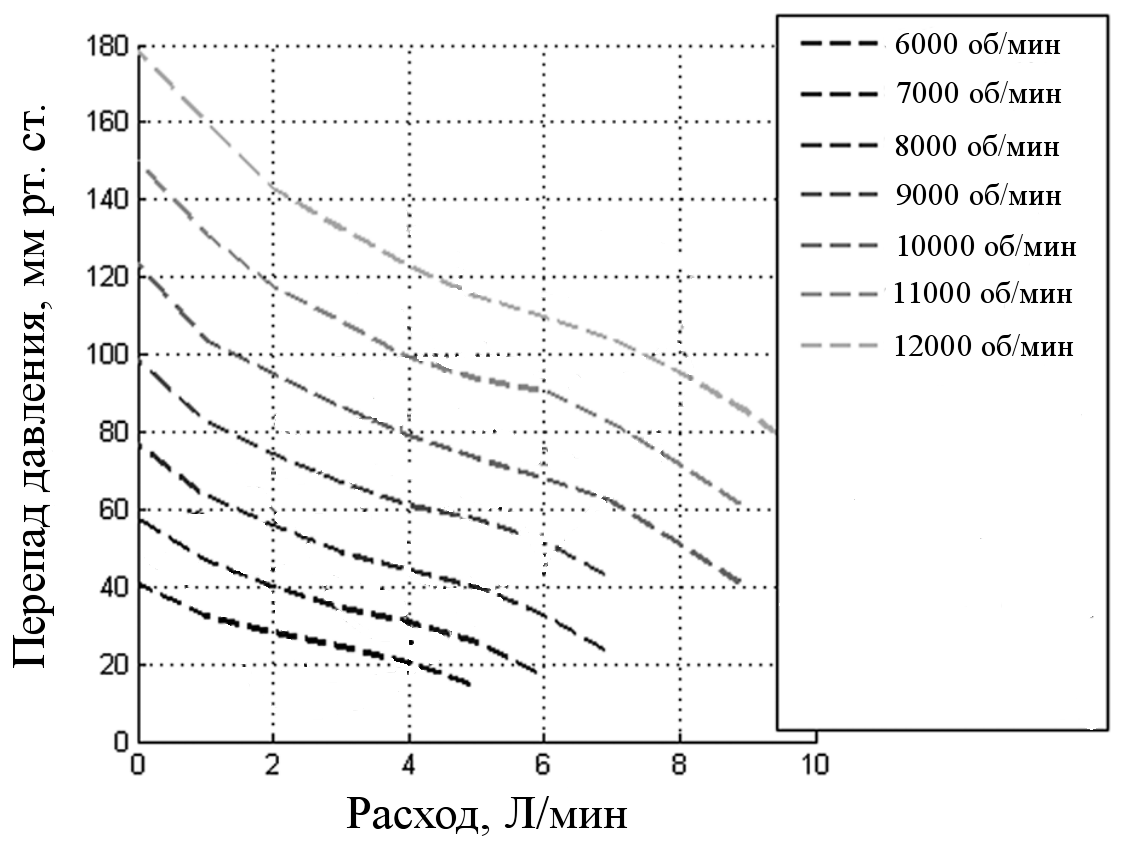
\includegraphics [scale=0.35] {../images/c2_basic_hq_static} \\ а)}
  \end{minipage}
  \hfill
  \begin{minipage}[ht]{0.48\linewidth}
    \center{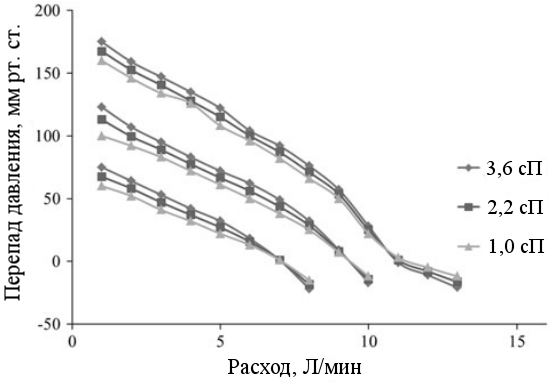
\includegraphics [scale=0.43] {../images/c2_basic_hq_static_viscosity} \\ б)}
  \end{minipage}
  \caption{Расходно-напорные характеристики имплантируемого роторного насоса крови HeartMate II из работы Pennings и др. \cite{Pennings_2013} и Stanfield и др. \cite{Stanfield_2012}}
  \label{img:initial_data}  
\end{figure}

Влияние вязкости жидкости, перекачиваемой насосом при различных величинах скорости вращения ротора, показано на рисунке \ref{img:initial_data}б. Так, изменение вязкости от 3,6 до 1,0 сП приводит к изменению наклона рассматриваемой характеристики. В случае уменьшения вязкости до 1,0 сП при фиксированном перепаде давления (например, 100 мм рт. ст.) происходит уменьшение расхода примерно на 1-1,2 л/мин. С уменьшением перепада давления влияние вязкости уменьшается, однако при отрицательном перепаде давлений влияние вязкости крови прямо противоположно: ее уменьшение приводит к увеличению расхода при фиксированном перепада давления. 

Необходимость учета влияния вязкости жидкости при разработке математических моделей имплантируемых роторных насосов крови обосновывается в работах \cite{Malagutti_2007, Pennings_2013, 4352467}. О необходимости учета влияния вязкости жидкости был сделан доклад на конференции <<МедТех>> \cite{medtech_2014}.

В ходе анализа ранее опубликованных работ \cite{Moscato_2009, Pirbodaghi_2011} для описания РНХ имплантируемого роторного насоса крови было выбрано следующее уравнение:

\begin{equation}
	\label{eq:initial_eq}
	L\frac{dQ}{dt} = (a_1\mu+a_2)Q + (b_1\mu+b_2)\omega^2 + H,
\end{equation}

\noindent где $L$ -- параметр, характеризующий инерцию жидкости в данном насосе (мм рт. ст.$~\cdot$ мин$^2~\cdot$ л$^{-1}$) \cite{Moscato_2009}, $Q$ -- расход насоса (л/мин), $\mu$ -- параметр, характеризующий вязкость жидкости в насосе (сП), $\omega$ -- скорость вращения ротора насоса (об/мин), $H$ -- перепад давления в насосе (мм рт. ст.), $a$ и $b$ -- коэффициенты, представленные линейной функцией вида $x(\mu) = x_1\mu + x_2$, что позволяет учесть изменение в наклоне расходно-напорной характеристики при изменении вязкости жидкости ($\mu$, сП) \cite{Malagutti_2007}. 

Параметр $L$ выбран равным 0,2, значения коэффициентов уравнения \eqref{eq:initial_eq} определены с помощью процедуры оптимизации, описание которой приводится далее. Оптимизация коэффициентов уравнения проведена по точкам, которые были выбраны в ходе анализа расходно-напорных характеристик роторного насоса крови HeartMate II и отмечены круглыми маркерами на рисунке \ref{img:pump_identification_first_stage}.

Расходно-напорные характеристики, описываемые уравнением \eqref{eq:initial_eq}, представлены на рисунке \ref{img:pump_identification_first_stage}. 

% Так, параметр $L$ выбран произвольно и, согласно работе \cite{Moscato_2009}, для реального насоса он может быть другим. Влияние вязкости воспроизведено также примерно, хотя та динамика РНХ, которая наблюдается на экспериментальных кривых, повторяется моделью совершенно точно. 

\section[Процедура оптимизации]{Процедура оптимизации коэффициентов модели идентификации}

В ходе исследования была разработана процедура оптимизации коэффициентов математической модели идентификации на основе алгоритма Левенберга-Марквардта \cite{IMM2004, gavin2011levenberg}, которая позволяет обеспечить соответствие между выходными данными математической модели и набором искомых значений или экспериментальных данных. 

Основная задача алгоритма заключается в оптимизации вектора параметров $\beta$ целевой функции $f(x, \beta)$ относительно эмпирических значений $y$ таким образом, чтобы сумма вектора невязки $S(\beta)$ была минимальной:

\begin{equation}
	S(\beta) = \sum_{i=1}^{m} [y_i - f(x_i, \beta)]^2
\end{equation}

В качестве параметра $x$ целевой функции $f$ задан массив \verb!p1!, в качестве параметра $\beta$ -- массив \verb!v_i!. 

Подобно другим численным алгоритмам оптимизации, данный алгоритм является итерационной процедурой. Первоначально формируется начальное приближение для вектора параметров $\beta$. Предполагается, что для случая с только одним минимумом хорошо работает приближение вида $\beta = (1,0, 1,0, \ldots, 1,0)$.

На каждой итерации находится приращение $\delta$ к вектору параметров $\beta$. Основное уравнение алгоритма Левенберга-Марквардта выглядит следующим образом:

\begin{equation}
	(J^T J + \lambda ~diag(J^TJ))\delta = J^T[y-f(\beta)]
	\label{eq:lm_method}
\end{equation}

\noindent где $J$ -- матрица Якоби, $J^T$ -- транспонированная матрица Якоби, $\lambda$ -- коэффициент затухания, $\delta$ -- искомое приращение к вектору параметров $\beta$, $y$ -- искомые значения, $f$ -- целевая функция.

%В уравнении \eqref{eq:lm_method} используется диагональная матрица, содержащая диагональные элементы $J^TJ$. %, которая в данной работе в большинстве случаев заменена на матрицу идентичности $I$, т.\:е. используется версия алгоритма без модификации Марквардта. 

Значение каждого элемента матрицы Якоби описывается следующим уравнением: 

\begin{equation}
	J_i = \frac{\partial f(x_i, \beta)}{\partial \beta}
\end{equation}

Исходное неотрицательное значение коэффициента затухания $\lambda$ установлено эмпирически. Значение коэффициента может быть изменено на каждой итерации. Например, в случае быстрого уменьшения суммы вектора невязки значение коэффициента может быть уменьшено. 

Матрица Якоби вычисляется как разность между векторами невязок \verb!r! и \verb!rr!. Вектор невязки \verb!r! вычисляется как разность между массивом значений целевой функции \verb!M!, полученных с использованием вектора параметров \verb!p_i!, и массивом искомых значений \verb!T!. Вектор невязки \verb!rr! вычисляется с использованием вектора параметров \verb!pp_i!, полученных в результате отклонения массива \verb!v_i! на шаг \verb!dx!. 

Для перемножения матриц используется функция \verb!dot! из библиотеки NumPy, для нахождения приращения \verb!s! -- функция \verb!lstsq! из библиотеки NumPy.

Целевая функция может быть критична к выбору параметров \verb!v_i!, например, они должны быть неотрицательны. Чтобы учесть это были введены проверки на величину приращений \verb!s!: если оно больше, чем значение соответствующего параметра \verb!v_i!, то оно делится на десять -- данное значение подобрано эмпирически и может быть любым. 

Процедура оптимизация реализована на языке программирования Python с использованием библиотеки NumPy. Программный код приведен в приложении \ref{list:optimization_routine}. При разработке использованы результаты диссертационной работы W. Smith <<Minimal heamodynamic modelling of the heart \& circulation for clinical applications>>.

\section{Алгоритм структурно-параметрической идентификации}

В ходе анализа полученных результатов было установлено несоответствие между формой моделируемых расходно-напорных характеристик, представленных на рисунке \ref{img:pump_identification_first_stage}, и формой исходных РНХ, представленных на рисунке \ref{img:initial_data}. 

\begin{figure}[ht]
  \center{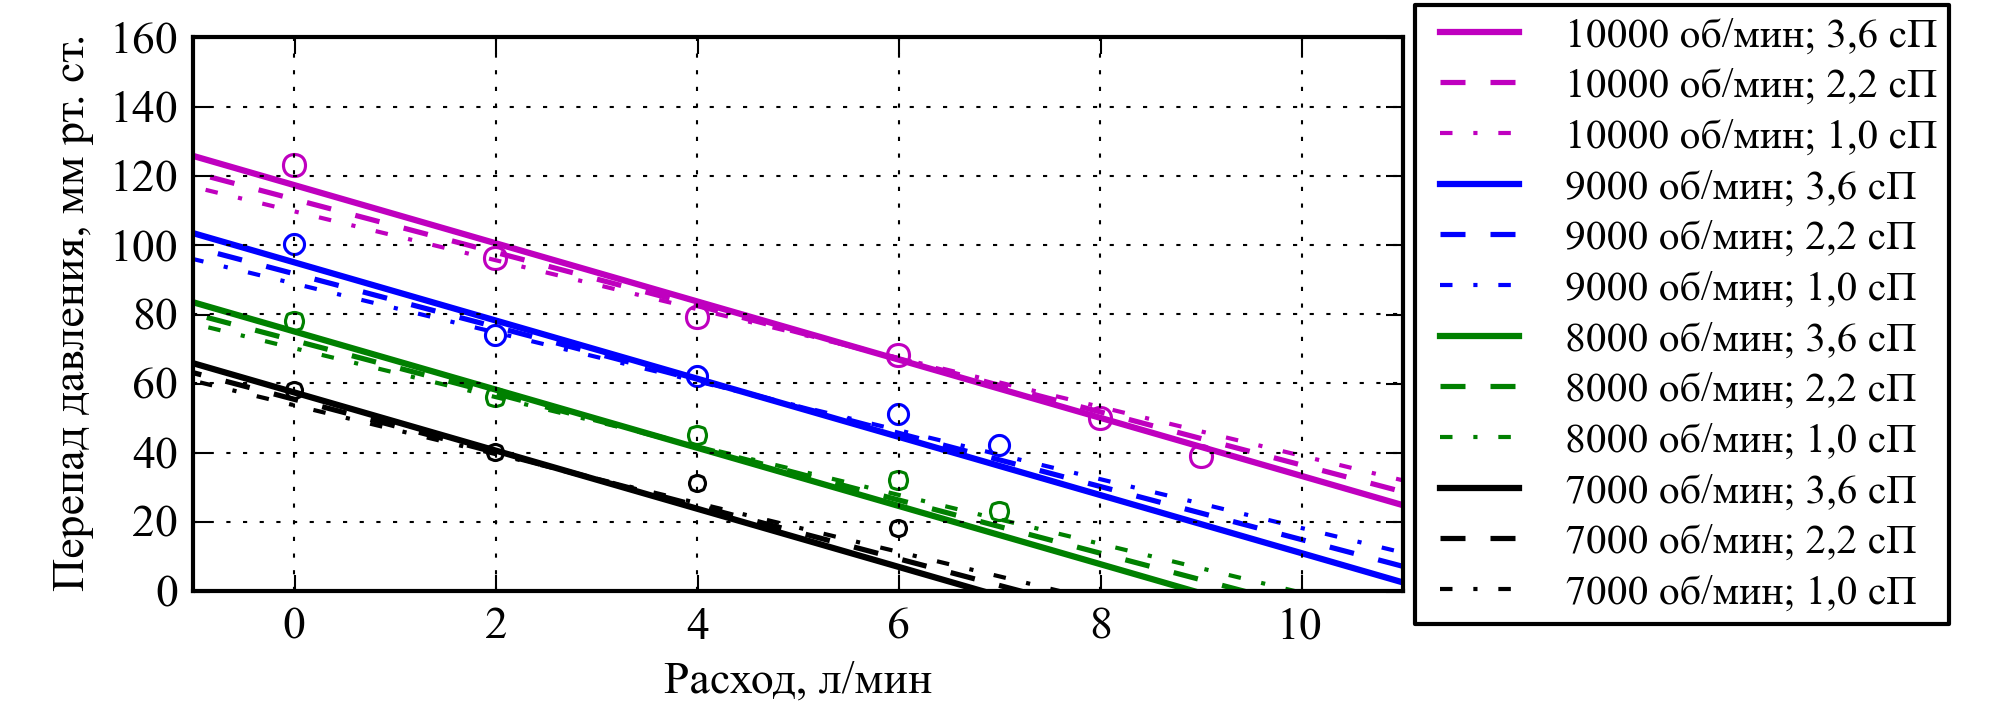
\includegraphics [scale=0.99] {../images/c2_static_model_initial_dis}}
  \caption{Расходно-напорные характеристики роторного насоса крови, описываемые уравнением \eqref{eq:initial_eq}}
  \label{img:pump_identification_first_stage}  
\end{figure}

Решением данной проблемы стала разработка алгоритма структурно-параметрической идентификации. Основная идея алгоритма заключается в последовательном добавлении одночленов $kx_j$ к исходному уравнению $y_i$ и отборе уравнений вида $y_i + kx_j$ посредством сравнения с критерием оценки эффективности идентификации на каждой итерации алгоритма $i$. 

Схема алгоритма идентификации представлена на рисунке \ref{img:flowchart}.

\begin{figure}[!ht]
\centering
\begin{tikzpicture}[node distance=1cm, auto]  

\tikzstyle{startstop} = [rectangle, rounded corners=10pt, minimum width=3.0cm, minimum height=1.35cm,text centered, draw=black]
\tikzstyle{io} = [trapezium, trapezium left angle=70, trapezium right angle=110, minimum width=0.9cm, minimum height=1.1cm, text centered, draw=black]
\tikzstyle{process} = [rectangle, minimum width=1.1cm, minimum height=1.3cm, text centered, draw=black]
\tikzstyle{decision} = [diamond, minimum width=3.1cm, minimum height=1.35cm, text centered, draw=black]
\tikzstyle{arrow} = [thick,->,>=stealth]

\node (s) [startstop, yshift=-20.0, minimum height=0.9cm] {\parbox{4.5cm}{\small \centering Начало}};
\node (start) [process, below of=s, yshift=-20.0] {\parbox{5.95cm}{\small Задание исходного уравнения $y_i$ где $i$ -- номер итерации }};
\node (in1) [io, below of=start, yshift=-1.05cm] {\parbox{5.55cm}{\small Добавление к $y_i$ одночлена $kx_j$ где $k$ -- коэффициент \\ $j$ -- номер одночлена}};
\node (pro1) [process, below of=in1, yshift=-1.50cm] {\parbox{7.80cm}{\small Определение коэффициентов $y_i + kx_j$ с \\использованием процедуры оптимизации \\ Проверка соответствия критерию оценки эффективности идентификации}};
\node (dec1) [decision, below of=pro1, yshift=-1.30cm] {};% {\footnotesize\bf \parbox{1.5cm}{Соответствие \\ критериям}};
\node (dec2) [decision, below of=dec1, yshift=-0.75cm] {};
\node (out2a) [process, right of=dec2, yshift=0.0cm, xshift=5.2cm, minimum width=1.0cm] {\parbox{4.15cm}{\small Задание $y_i + kx_j$ \\исходным уравнением \\ $i = i + 1$ \\ $j = j + 1$}};
\node (out2b) [io, left of=dec1, xshift=-5.3cm, minimum width=1.0cm] {\parbox{3.70cm}{\small Исключение $y_i + kx_j$ \\ $j = j + 1$}};
\node (out2c) [process, below of=dec2, yshift=-0.8cm, minimum height=1.0cm] {\small Окончательное $y_i + kx_j$};
\node (out) [startstop, below of=out2c, yshift=-0.5cm, minimum height=0.9cm] {\parbox{4.5cm}{\small \centering Конец}};

\draw [arrow] (s) -- (start);
\draw [arrow] (start) -- (in1);
\draw [arrow] (in1) -- (pro1);
\draw [arrow] (pro1) -- (dec1);
\draw [arrow] (out2c) -- (out);
\draw [arrow] (dec2) -- node[anchor=south] {\small нет} (out2a);
\draw [arrow] (dec1) -- node[anchor=south] {\small нет} (out2b);
\draw [arrow] (dec1) -- node[anchor=west] {\small ~да} (dec2);
\draw [arrow] (dec2) -- node[anchor=west] {\small ~да} (out2c);
\draw [arrow] (out2a) |- ($(in1.east)+(0,-0.1)$);
\draw [arrow] (out2b) |- ($(in1.west)+(0.05,0.1)$);
%\draw [arrow] (out2b) ($(out2b.east)$)|- + (2.5,0) |- ($(in1.east)+(0.05,0.1)$); 
\draw (0.0, -9.33) node {\small $R^2_{ij} > R^2_i$}; %  \\ $\delta(PS) \geq 85\%$
\draw (0.0, -11.05) node {\small $R^2_{ij} \geq 0,9980$}; %  \\ $\delta(PS) \geq 85\%$
\end{tikzpicture} 
\caption{Схема алгоритма идентификации роторного насоса крови} 
\label{img:flowchart}  
\end{figure}

%Работа алгоритма завершается в случае соответствия требуемой величине $R^2$.

В качестве исходного уравнения $y_i$ было выбрано уравнение \eqref{eq:initial_eq}. Список одночленов $kx_j$ был сформирован в результате анализа математических моделей роторных насосов крови, описанных в литературе и рассмотренных в разделе \ref{identification_review}. Каждый одночлен представляет собой произведение коэффициента $k$ и переменной $Q$, $\omega$ или $H$, возведенной в степень натурального числа.

В качестве критерия оценки эффективности идентификации, отражающего качество аппроксимации исходных данных и позволяющего завершить работу алгоритма, выбран коэффициент детерминации $R^2$:

\begin{equation}
	\label{eq:r_squared}
		R^2 = 1- \frac{{\sum\limits_{i=1}^n} (Q_i - \hat{Q_i})^2}{{\sum\limits_{i=1}^n} (Q_i - \tilde{Q_i})^2}, %~~~~\widetilde{Q_i} = \frac{1}{n} \sum\limits_{i=1}^n Q_i
\end{equation}

\noindent где $Q_i$ -- прогноз математической модели, $\hat{Q_i}$ -- фактические значения, $\tilde{Q_i}$ -- среднее арифметическое значение прогнозов математической модели \cite{draper2014applied}. 

В ходе моделирования расходно-напорных характеристик пороговое значение коэффициента детерминации было выбрано равным 0,9980 и более, поскольку при данных значениях достигалось соответствие моделируемых и экспериментальных РНХ и, таким образом, точная идентификация характеристик насоса.

\subsection{Результаты идентификации}

С математической моделью, представленной уравнением \eqref{eq:initial_eq}, было достигнуто значение $R^2$ равное 0,9566; моделируемые расходно-напорные характеристики представлены на рисунке \ref{img:pump_identification_first_stage}, где круглыми маркерами отмечены точки, по которым проводилась идентификация. 

После этого к уравнению \eqref{eq:initial_eq} были добавлены члены $Q^2$ и $Q^3$:

\begin{equation}
	\label{eq:first_step_pump_model}
	L\frac{dQ}{dt} = (a_1\mu+a_2)Q + (b_1\mu+b_2)\omega^2 + (c_1\mu+c_2)Q^2 + (d_1\mu+d_2)Q^3 - H.
\end{equation}

%  Уравнение решалось с помощью функции \verb!fsolve! из программной библиотеки SciPy. Примерный вид полученных статических РНХ приведен на рисунке \ref{img:static_model}а. Пустыми черными круглыми маркерами отмечены точки, по которым проводилась оптимизация.

Это позволило увеличить $R^2$ до 0,9738 и моделировать $S$-образный изгиб расходно-напорной характеристики насоса, наблюдаемый на рисунке \ref{img:initial_data}а и характерный для роторных насосов крови с осевым направлением течения \cite{Pennings_2013}. Полученные расходно-напорные характеристики представлены на рисунке \ref{img:pump_identification_second_stage}.

\begin{figure}[ht]
  \center{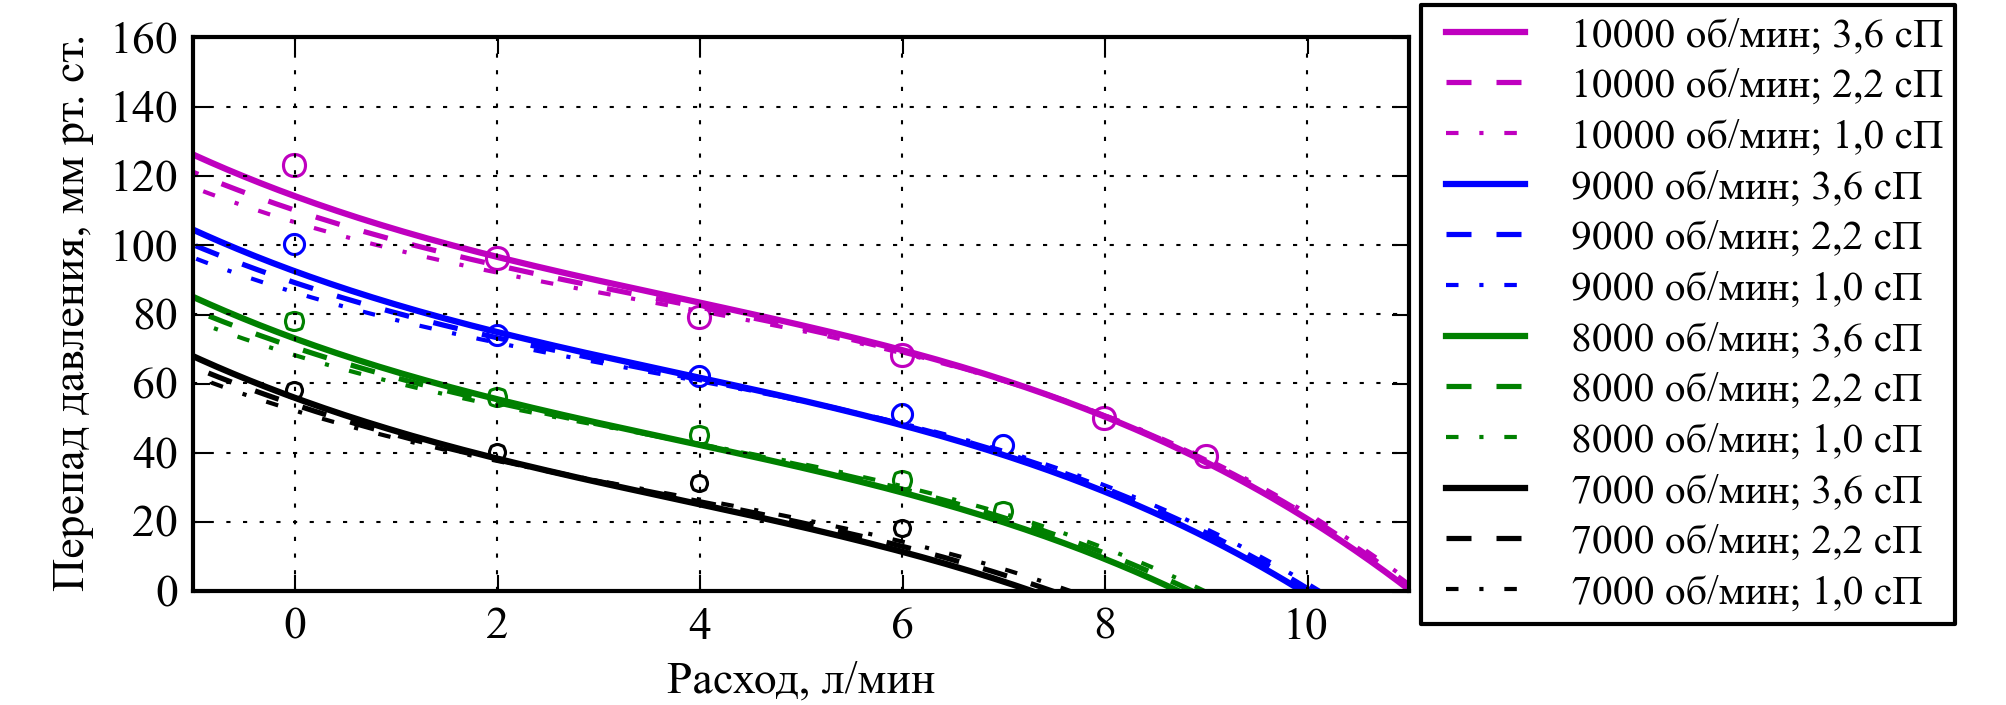
\includegraphics [scale=0.99] {../images/c2_static_model_updated_dis} \\ б)}
  \caption{Расходно-напорные характеристики роторного насоса крови, описываемые уравнением \eqref{eq:first_step_pump_model}}
  \label{img:pump_identification_second_stage}  
\end{figure}

После этого к уравнению \eqref{eq:first_step_pump_model} были добавлены члены $Q\omega^2$ и $Q^2 \omega$ вместе с поправочным коэффициентом $g = g_1\mu + g_2$, что позволило увеличить $R^2$ до 0,9987.% Полученные расходно-напорные характеристики представлены на рисунке \ref{img:pump_identification_second_stage}.

В результате было достигнуто соответствие между формой моделируемых и исходных РНХ и работа алгоритма была завершена. 

Разработанная в результате идентификации математическая модель роторного насоса крови описывается следующим уравнением: 

\begin{multline}
 L\frac{dQ}{dt} = (a_1\mu+a_2)Q + (b_1\mu+b_2)Q^2 + (c_1\mu+c_2)Q^3 + (d_1\mu+d_2)\omega^2 \\+ (e_1\mu+e_2)Q\omega^2 + (f_1\mu+f_2)Q^2\omega + g_1\mu+g_2 - H.
\label{eq:final_pump_model}
\end{multline}

Разработанная модель идентификации описывает расходно-напорные характеристики, представленные на рисунке \ref{img:final_pump_model}.

\begin{figure}[ht] 
  \center
  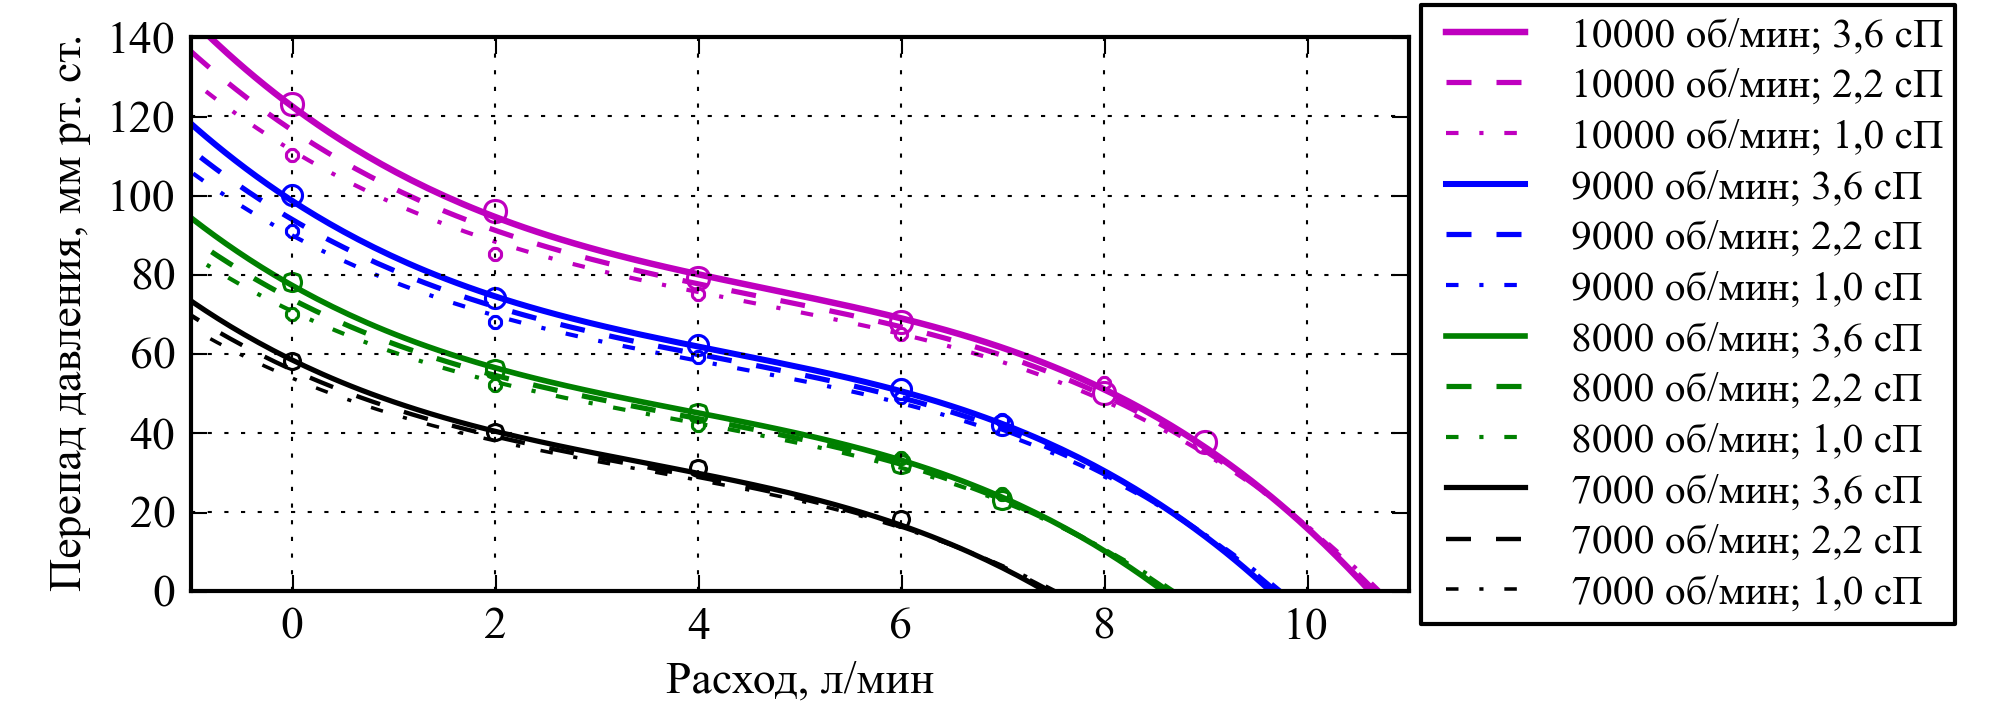
\includegraphics [scale=1.0] {../images/c2_static_model_final_dis}
  \caption{Расходно-напорные характеристики роторного насоса крови, описываемые уравнением \eqref{eq:final_pump_model}} 
  \label{img:final_pump_model}  
\end{figure}

Значения коэффициентов $a$, $b$, $c$, $d$, $e$, $f$ и $g$ приведены в таблице \ref{tbl:pump_model_coefficients}. 

\begin{table} [htbp]%
    \centering
	\caption{Коэффициенты математической модели роторного насоса крови}%
	\label{tbl:pump_model_coefficients}% label всегда желательно идти после caption
    \renewcommand{\arraystretch}{1.5} 
	\begin{tabular}{@{}@{\extracolsep{20pt}}llll@{}} 
        \toprule     %%% верхняя линейка
    	Коэффициент & Значение \\
        \midrule %%% тонкий разделитель. Отделяет названия столбцов. Обязателен по ГОСТ 2.105 пункт 4.4.5 
    	$a = a_1 + a_2\mu$ & $a_1 = -6,2332$ мм рт. ст. л$^{-1}$ \\
		 & $a_2 = -0,0254$ мм рт. ст. л$^{-1}$ сП$^{-1}$  \\
		$b = b_1 + b_2\mu$ & $b_1 = 0,5339$ мм рт. ст. л$^{-2}$  \\
		 & $b_2 = -0,0239$ мм рт. ст. л$^{-2}$ сП$^{-1}$  \\
    	$c = c_1 + c_2\mu$ & $c_1 = -0,1594$ мм рт. ст. л$^{-3}$ \\
		 & $c_2 = -0,0147$ мм рт. ст. л$^{-3}$ сП$^{-1}$  \\
		$d = d_1 + d_2\mu$ & $d_1 = 1,0778$ мм рт. ст. мин$^{2}$  \\
		 & $d_2 = 0,0495$ мм рт. ст. мин$^{2}$ сП$^{-1}$  \\
    	$e = e_1 + e_2\mu$ & $e_1 = -0,0788$ мм рт. ст. мин$^2$ л$^{-1}$ \\
		 & $e_2 = -0,0133$ мм рт. ст. мин$^2$ л$^{-1}$ сП$^{-1}$  \\
		$f = f_1 + f_2\mu$ & $f_1 = 0,1568$ мм рт. ст. мин л$^{-2}$ \\
		 & $f_2 = 0,0263$ мм рт. ст. мин л$^{-2}$ сП$^{-1}$ \\
    	$g = g_1 + g_2\mu$ & $g_1 = -0,6583$ мм рт. ст. \\
		 & $g_2 = -0,6671$ мм рт. ст. сП$^{-1}$  \\
        \bottomrule %%% нижняя линейка
	\end{tabular}%
\end{table}

Поскольку состояние РНК описывается единственной переменной $Q$, то фазовое пространство уравнения \eqref{eq:final_pump_model} одномерно и представлено вещественной прямой $0Q$. Поэтому для наглядности будем изображать эволюцию уравнения \eqref{eq:final_pump_model}, откладывая по оси абсцисс время $t$, по оси ординат -- фазовую переменную $Q$:

\begin{figure}[ht] 
  \center
  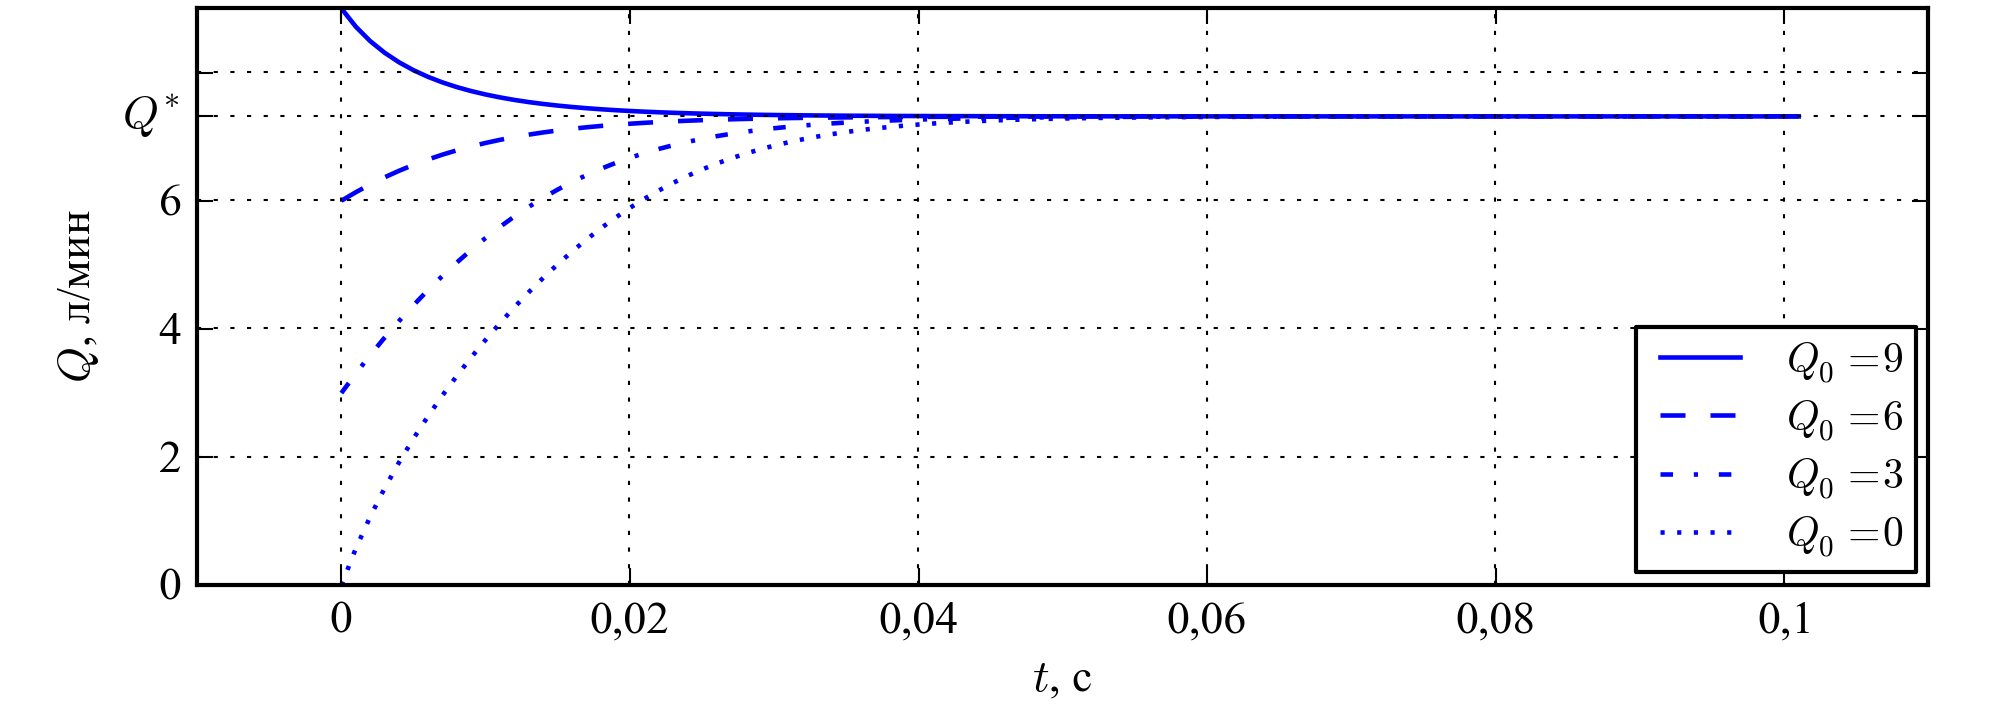
\includegraphics [scale=1.0] {../images/c2_dynamic_model_solution_zero}
  \caption{Зависимость $Q$ от времени при различных начальных условиях}
  \label{img:final_pump_model_solution_zero}  
\end{figure}

На рисунке \ref{img:final_pump_model_solution_zero} представлено изменение $Q$ от времени $t$ при различных начальных значениях $Q_0$ и фиксированных параметрах $\mu = $ 3,6 сП, $\omega =$ 8000 об/мин и $H = $ 20 мм рт. ст. Видно, что с течением времени значения переменной $Q$ стремятся к некоторому особому значению $Q^*$. При этом значения достаточно быстро выходят на $Q^*$. 

Найдем особые точки уравнения \eqref{eq:final_pump_model}, приравняв левую часть уравнения \eqref{eq:final_pump_model} к нулю:

\begin{multline}
(a_1\mu+a_2)Q + (b_1\mu+b_2)Q^2 + (c_1\mu+c_2)Q^3 + (d_1\mu+d_2)\omega^2 + \\+ (e_1\mu+e_2)Q\omega^2 + (f_1\mu+f_2)Q^2\omega + g_1\mu+g_2 - H = 0.
\label{eq:final_pump_model_zero}
\end{multline}

Уравнение \eqref{eq:final_pump_model_zero} решено с использованием формулы Кардано для нахождения корней $x_1$, $x_2$ и $x_3$ уравнения вида $ax^3 + bx^2 + cx + d = 0$:

\begin{equation}
x_1 = -\frac{b}{3a} + \alpha + \beta, \quad x_{2, 3} = -\frac{b}{3a}  - \frac{(\alpha + \beta)}{2} \pm \frac{i(\alpha - \beta)}{2}\sqrt{3},
\label{eq:cardano_1}
\end{equation}

где 

\begin{equation}
a = c_1\mu + c_2, \quad b = b_1\mu + b_2 + (f_1\mu + f_2)\omega,
\label{eq:cardano_2_1}
\end{equation}

\begin{equation}
c = a_1\mu + a_2 + (e_1\mu + e_2)\omega^2, \quad d = (d_1\mu + d_2)\omega^2 + g_1\mu + g_2 - H,
\label{eq:cardano_2_2}
\end{equation}

\begin{equation}
\alpha = \sqrt[3]{-\frac{q}{2} + \sqrt{R}}, \quad \beta = \sqrt[3]{-\frac{q}{2} - \sqrt{R}},
\label{eq:cardano_2}
\end{equation}

\begin{equation}
R = \left(\frac{p}{3}\right)^3 + \left( \frac{q}{2} \right)^2,
\label{eq:cardano_3}
\end{equation}

\begin{equation}
p = \frac{3ac - b^2}{3a^2}, \quad q = \frac{2b^3 - 9abc + 27a^2d}{27a^3}.
\label{eq:cardano_extension}
\end{equation}

По знаку $R$ можно определить тип корней. Если член $p$ больше нуля, то $R$ заведомо больше нуля и решение уравнения \eqref{eq:final_pump_model_zero} имеет один вещественный корень и два сопряженных комплексных корня. % \cite{korn1973}.

Так, в член $p$ входят параметры $\mu$ и $\omega$: параметр $\mu$ изменяется в диапазоне от 1,0 сП до 3,6 сП, параметр $\omega$ -- от 5 до 11 тысяч об/мин. На рисунке \ref{img:model_zero_roots} представлены зависимости $p$ для физически реализуемых $\mu$ и $\omega$.

\begin{figure}[ht] 
  \center
  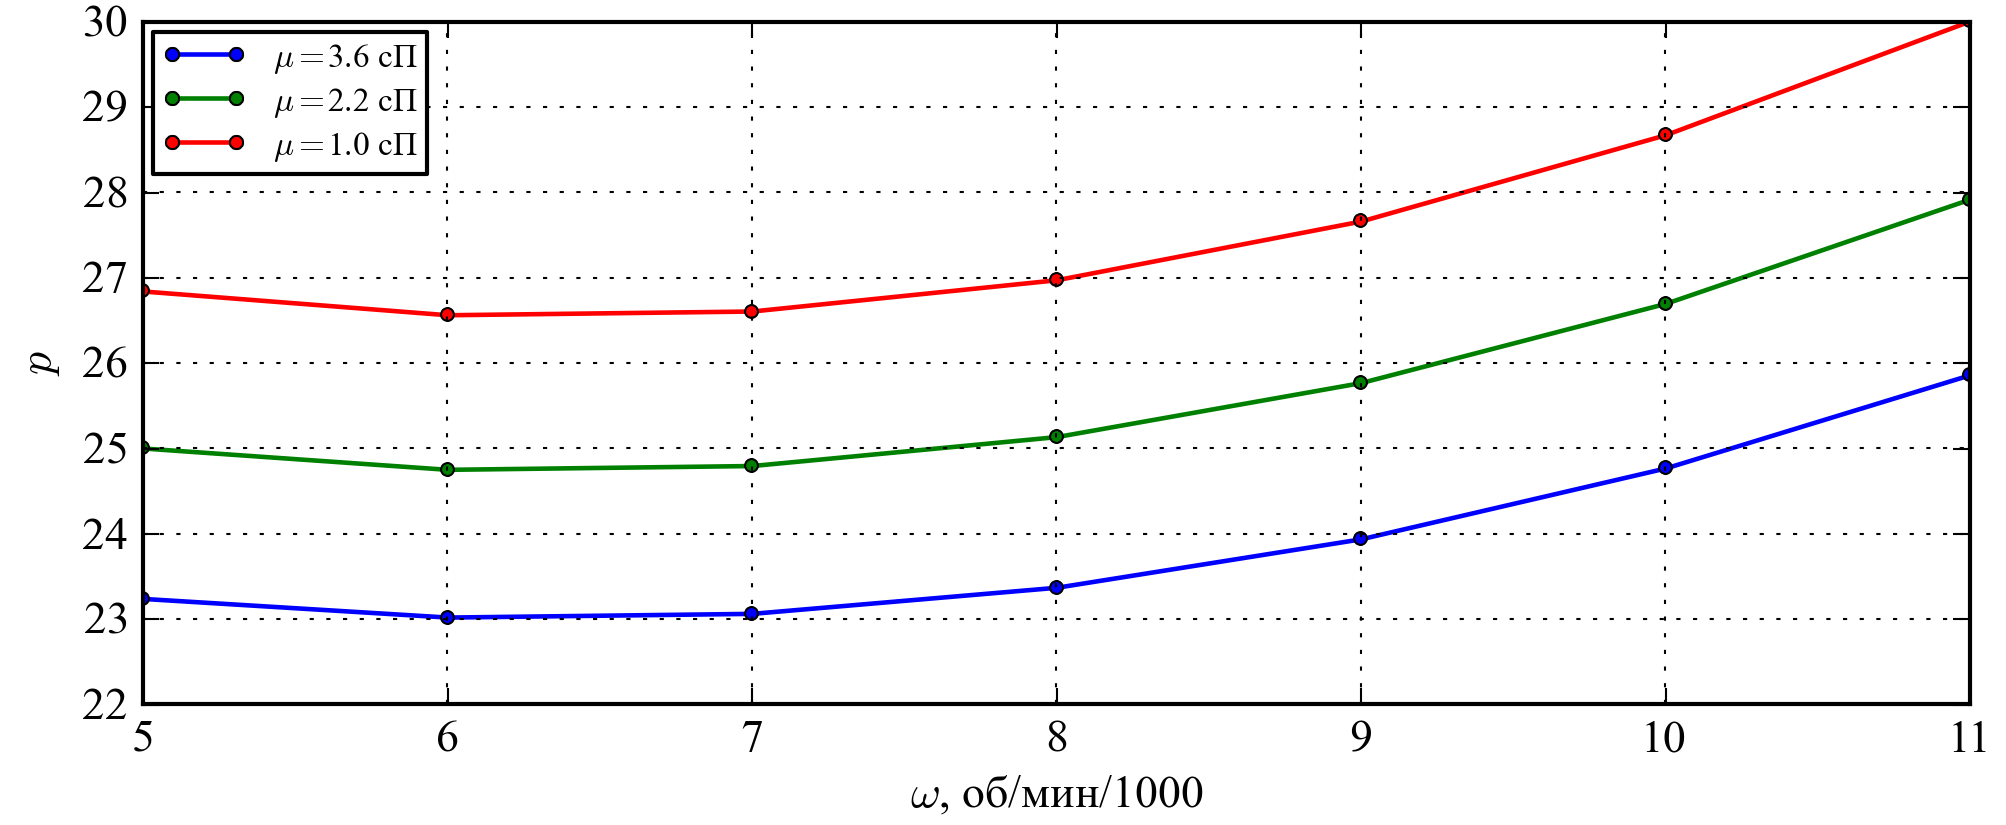
\includegraphics [scale=1.0] {../images/c2_model_zero}
  \caption{Зависимость $p$ для физических реализуемых параметров $\mu$ и $\omega$}
  \label{img:model_zero_roots}  
\end{figure}

Для уравнения \eqref{eq:final_pump_model_zero} $R > 0$, таким образом, уравнение \eqref{eq:final_pump_model_zero} имеет один вещественный корень и два сопряженных комплексных корня, следовательно, при всех физически реализуемых $\mu$, $\omega$ и $H$ особая точка уравнения \eqref{eq:final_pump_model} единственна.

%\section*{Влияние вязкости жидкости на расходно-напорную характеристику роторного насоса крови} \label{subsect2_1_1} 

% Поскольку разработанная математическая модель учитывает инерционные и вязкостные свойства крови в данной главе демонстрируется и дается количественная оценка влияния инерционных и вязкостных свойств крови на величину потока через РНК. 
% 
% Количественная оценка влияния вязкости крови на величину потока через роторный насос крови приведена на рис. \ref{img:viscosity_main} при скоростях от 5 до 9 тысяч об/мин в диапазоне вязкостей от 3,6 до 1,0 сП. Влияние изменения вязкости крови на величину потока через насоса при изменении частоты сердечных сокращений и сократимости левого желудочка сердца -- на рис. \ref{img:viscosity_HR_CV}.
% 
% \begin{figure}[ht] 
%   \center
%   \includegraphics [scale=1.0] {../images/c2_viscosity_main}
%   \caption{Влияние изменения вязкости крови $\mu$ на величину потока через насос при различных скоростях насоса} 
%   \label{img:viscosity_main}  
% \end{figure}
% 
% Видно, что уменьшение вязкости с 3,6 до 1,0 сП при фиксированной скорости приводит к уменьшению минутной расхода насоса: на 0,1 л/мин при 6000 об/мин и на 0,22 л/мин при 8000 об/мин. Таким образом, чем выше скорость насоса, тем сильнее изменение $\mu$ влияет на величину потока. Тем не менее, при 9000 об/мин влияние вязкости крови незначительно уменьшается -- до 0,09 л/мин. 
% 
% Кроме того, увеличение частоты сердечных сокращений с 60 уд/мин до 100 уд/мин также приводит к большему влиянию величины вязкости на минутный расход насоса: уменьшение $\mu$ с 3,6 до 1,0 сП при 8000 об/мин уменьшает расход на 0,25 л/мин. Влияние сократимости левого желудочка сердца аналогично ЧСС: увеличение параметра $C_V$ на 10\% приводит к усилению вязкости крови на расход насоса.
% 
% \begin{figure}[ht] 
%   \center
%   \includegraphics [scale=1.0] {../images/c2_viscosity_HR_CV}
%   \caption{Влияние изменения вязкости крови $\mu$ на величину потока через насос при различных скоростях насоса и изменении частоты сердечных сокращений (ЧСС, уд/мин) и сократимости левого желудочка сердца ($C_V$, \%)} 
%   \label{img:viscosity_HR_CV}  
% \end{figure}
% 
% Таким образом, усиление сердечной функции, независимо от того обусловлено ли оно увеличением ЧСС или сократимости ЛЖ, приводит к увеличению влияния вязкости крови на минутный расход насоса.  
% 
% Количественная оценка влияния параметра $L$ на величину потока через роторный насос крови приведена на рис. \ref{img:inertia_main} при скоростях от 5 до 9 тысяч об/мин в диапазоне параметра $L$ от 0.2 до 0.8. Влияние изменения $L$ на величину потока через насоса при изменении частоты сердечных сокращений и сократимости левого желудочка сердца -- на рис. \ref{img:inertia_HR_CV}.
% 
% \begin{figure}[ht] 
%   \center
%   \includegraphics [scale=1.0] {../images/c2_inertia_main}
%   \caption{Влияние изменения параметра $L$ на величину потока через насос при различных скоростях насоса} 
%   \label{img:inertia_main}  
% \end{figure}
% 
% \begin{figure}[ht] 
%   \center
%   \includegraphics [scale=1.0] {../images/c2_inertia_HR_CV}
%   \caption{Влияние изменения параметра $L$ на величину потока через насос при различных скоростях насоса и изменении частоты сердечных сокращений (ЧСС, уд/мин) и сократимости левого желудочка сердца ($C_V$, \%)} 
%   \label{img:inertia_HR_CV}  
% \end{figure}
% 
% Видно, что увеличение параметра $L$ до 0,8 приводит к уменьшению минутного расхода насоса в диапазоне скоростей от 5000 до 8000 об/мин. В то же время, его влияние уменьшается с увеличением скорости насоса до 9000 об/мин, при этом увеличение $L$ приводит к незначительному увеличению расхода на 0,04 л/мин.
% 
% Увеличение частоты сердечных сокращений и сократимости ЛЖ также приводит к увеличению влияния параметра $L$. В этом случае при ЧСС 100 уд/мин и скорости 6000 об/мин увеличение $L$ до 0.8 уменьшает расхода насоса на 0,32 л/мин. Аналогичным образом, влияние параметра $L$ уменьшается с увеличением скорости насоса и минимальное изменение минутного расхода при увеличении $L$ до 0,8 составляет 0,08 л/мин (скорость 8000 об/мин и ЧСС 60 уд/мин).
% 
% На рис. \ref{img:L_mu_influence} продемонстрировано влияние вязкости крови при различных величинах параметра $L$. Во всех случаях уменьшение вязкости крови до 1,0 сП приводит к уменьшению минутного расхода насоса; при этом увеличение скорости также усиливает влияние вязкостных свойств крови на минутный расхода насоса аналогично рис. \ref{img:viscosity_main}. В то же время, увеличение $L$ с 0.2 до 0.8 приводит к увеличению влияния вязкостных свойств крови. Самое малое изменение в расходе насоса на 0,15 л/мин происходит при уменьшении вязкости с 3,6 до 1,0 сП, скорости 6000 об/мин и $L$ = 0.2.
% 
% \begin{figure}[ht] 
%   \center
%   \includegraphics [scale=1.0] {../images/c2_L_mu_influence}
%   \caption{Влияние изменения вязкости крови $\mu$ на величину потока через насос при различных величинах скорости насоса и параметра $L$} 
%   \label{img:L_mu_influence}  
% \end{figure}
% 
% В данной главе также предлагается алгоритм управления расходом роторного насоса крови. Разработанная математическая модель РНК позволяет оценивать только мгновенный расход, поэтому реализация метода оценки потока в системе управления предполагает реализацию алгоритма управления расходом насоса. 
% 
% Структурная схема алгоритма управления расходом РНК показана на рис. \ref{img:simple_control_algorithm}. Она состоит из трех блоков. Основным компонентом блока РНК является математическая модель РНК, которая позволяет оценить поток в данный момент времени на основе значений скорости $\omega$, перепада давления $H$ и вязкости крови $\mu$, величина которой задается на внешней консоли управления.
% 
% В оценочном блоке производится оценка минутного ($Q_P$) и приближенного ($Q_A$) расходов РНК на основе временной диаграммы расхода, сформированной благодаря блоку РНК.   
% 
% \begin{figure}[ht] 
%   \center
%   \includegraphics [scale=1.7] {../images/c2_simple_control_algorithm}
%   \caption{Структурная схема алгоритма управления расходом роторного насоса крови}
%   \label{img:simple_control_algorithm}
% \end{figure}
% 
% На рис. \ref{img:flow_estimation} показаны два способа оценки минутного и приближенного расходов. В первом случае используется временная диаграмма расхода на временном промежутке в 60 секунд; интегрирование расходной характеристики в указанном диапазоне позволяет определить минутный расход насоса $Q_P$ (л/мин).
% 
% \begin{figure}[ht] 
%   \center
%   \includegraphics [scale=1.0] {../images/c2_flow_estimation}
%   \caption{Оценка (А) минутного расхода насоса ($Q_P$, л/мин) и (Б) приближенного расхода ($Q_A$, л/мин) по временной диаграмме расхода насоса (л/с)}
%   \label{img:flow_estimation}
% \end{figure}
% 
% Во втором случае на временной диаграмме находится минимум, который соответствует началу диастолической фазы сердечного цикла. Следующий минимум обозначает окончание данного сердечного цикла и начало новой диастолической фазы. Таким образом, можно определить промежуток времени, соответствующий определенному количеству сердечных циклов (в данном случае пяти). Из этих данных можно найти частоту сердечных сокращений и объем крови, который перекачан насосом за это время. Полученное значение аппроксимируется до литров в минуту и считается приближенным расходом насоса. 
% 
% В блоке регулировки скорости производится сравнение приближенного и требуемого уровня расхода $Q_D$, которое задается на внешней консоли управления. При их несовпадении происходит изменение скорости РНК на 100 об/мин.  
% 
% Пример использования данного способа оценки расхода с целью регулировки расхода насоса относительно требуемого значения при изменении физиологических условий показан на рис. \ref{img:estimated_flow_variation}. В этом случае изменение частоты сердечных сокращений от 60 уд/мин до 100 уд/мин при $Q_D =$ 3,8 л/мин приводит к соответствующими изменениями скорости РНК. 
% 
% \begin{figure}[ht] 
%   \center
%   \includegraphics [scale=1.0] {../images/c2_estimated_flow_variation}
%   \caption{Временная диаграмма изменения расхода ($Q_P$ и $Q_A$, л/мин), скорости насоса ($\omega_P$, об/мин/1000) и частоты сердечных сокращений (ЧСС, уд/мин)}
%   \label{img:estimated_flow_variation}
% \end{figure}
% 
% Видно, что уменьшение ЧСС до 60 уд/мин сопровождается уменьшением приближенного расхода относительно желаемого значения $Q_D$, поэтому скорость насоса начинает увеличиваться. Использование приближенного расхода $Q_A$ и его периодическое сравнение с $Q_D$ позволяет довольно быстро реагировать на физиологические изменения, такие как изменение ЧСС, и поддерживать расход РНК $Q_P$ на требуемом уровне.  

\section{Математические модели сердечной-сосудистой системы} \label{cvs_model_implementation}

В данной части приводится описание разработки математической модели сердечно-сосудистой системы с использованием математических моделей сердца и системы кровообращения.

\subsection*{Математическая модель системы кровообращения}

Система кровообращения описана математическими моделями с сосредоточенными параметрами на основе аналогии между течением крови в артерии и током в электрической цепи \cite{Kokalari_2013, shi2011review}. Пример такой аналогии представлен на рисунке \ref{img:blood_current_analogy}. Градиент давлений перемещает кровь из левого желудочка (ЛЖ) в аорту, преодолевая гидравлическое сопротивление так же, как и градиент напряжения в электрической цепи заставляет ток течь, преодолевая электрическое сопротивление. Таким образом, описывая давление и течение крови с помощью напряжения и тока, а эффекты трения, инерции крови и эластичность сосуда с помощью сопротивления $R$, индуктивности $L$ и емкости $C$ соответственно, можно использовать известные методы анализа электрических цепей для исследования кровообращения в сердечно-сосудистой системе. 

\begin{figure}[ht] 
  \center
  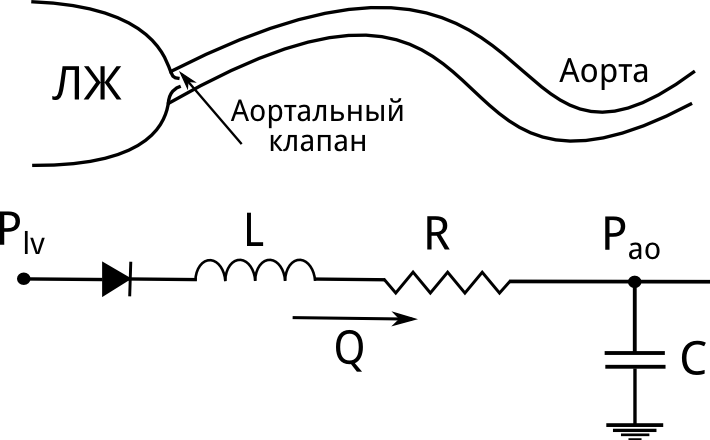
\includegraphics [scale=1.1] {../images/c2_electric_analogy}
  \caption{Пример аналогии между течением крови в аорте и током в электрической цепи; $P_{lv}$ -- давление в левом желудочке сердца, $P_{ao}$ -- давление в аорте, $L$ -- индуктивность, $R$ -- сопротивление, $C$ -- емкость, $Q$ -- поток}
  \label{img:blood_current_analogy}
\end{figure}

Математическая модель системы кровообращения представлена на рисунке \ref{img:full_cvs} в виде электрически-эквивалентной схемы аналогично работам \cite{Cox_2009, Martina_2013_simulation}. 

\begin{figure}[htb]
	\center{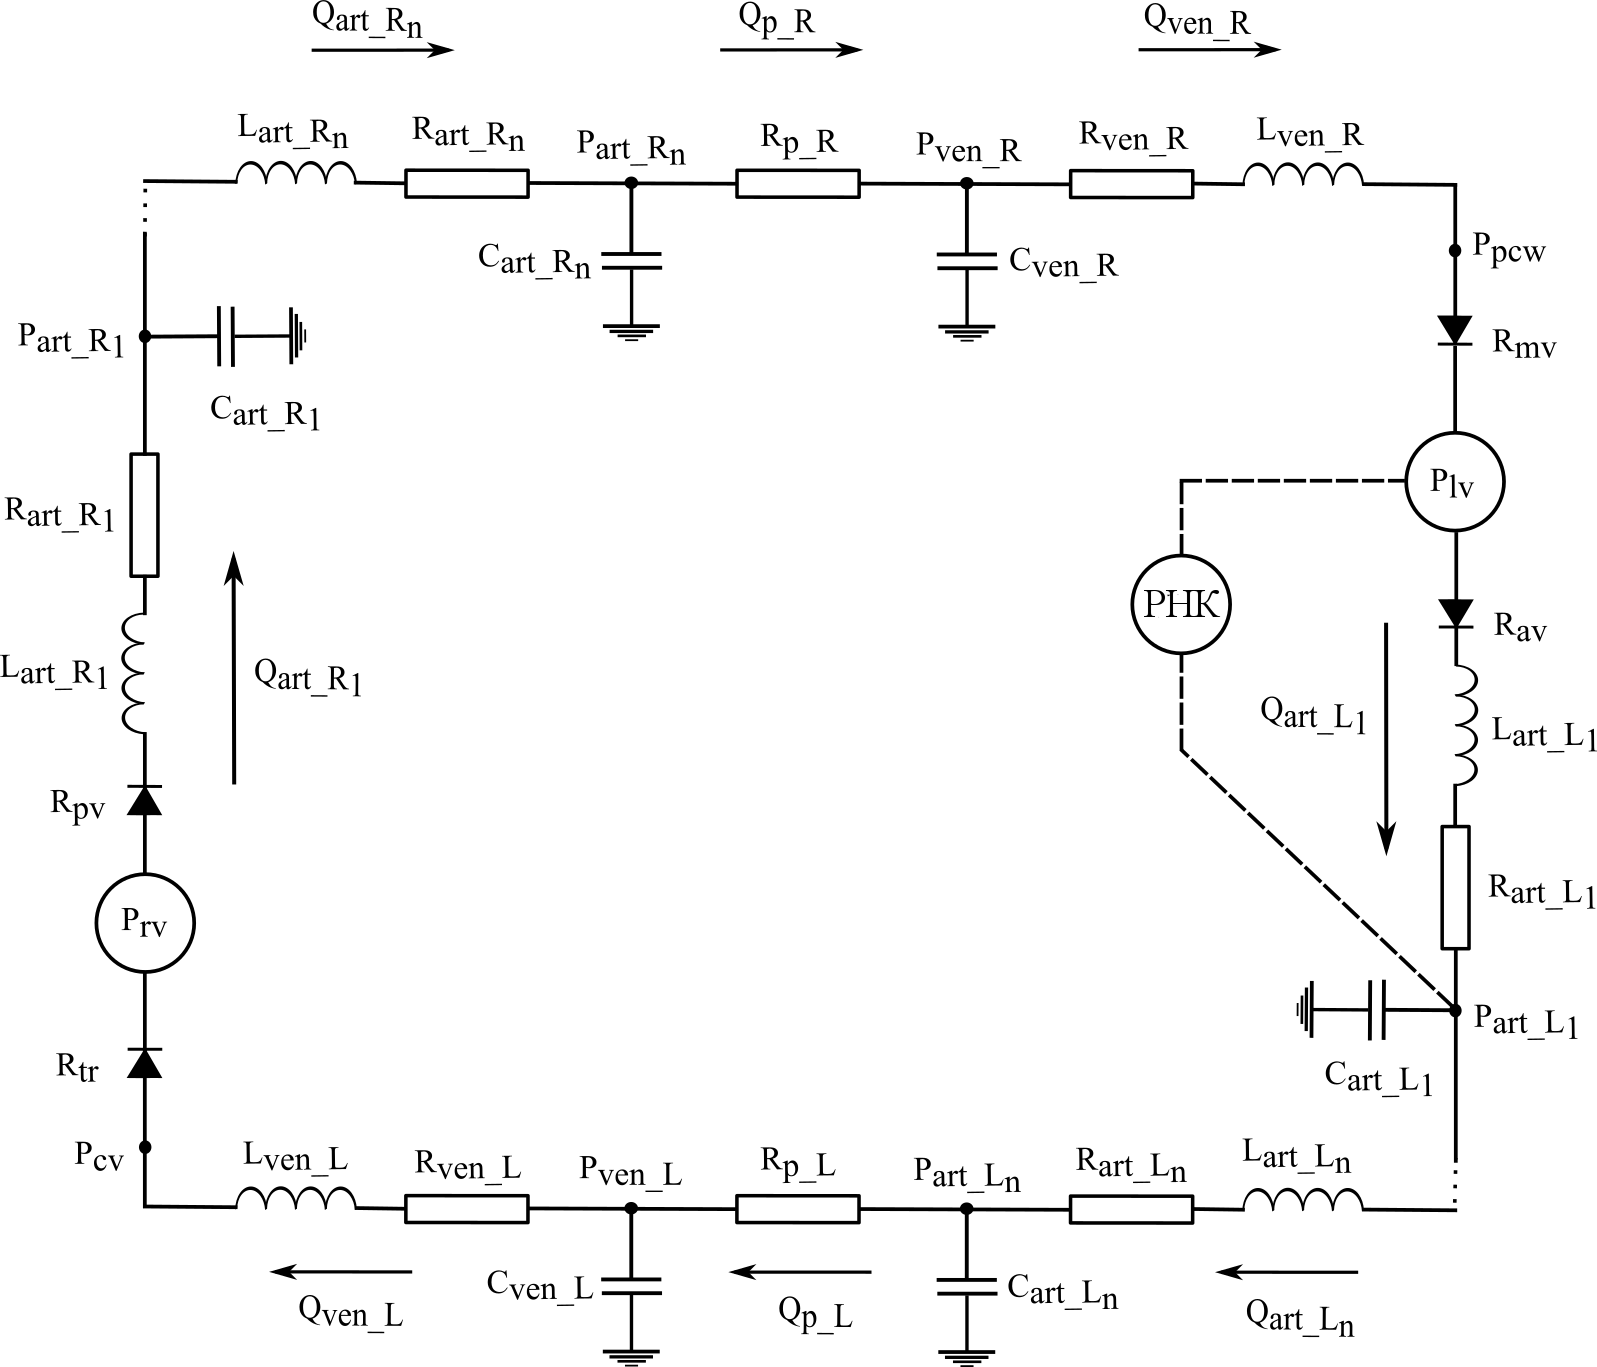
\includegraphics[width=1.0\linewidth]{../images/c2_cvs}}
	\caption{Математическая модель сердечно-сосудистой системы, представленная в виде электрически-эквивалентной схемы}
	\label{img:full_cvs}
\end{figure}

Большой и малый круги кровообращения составлены из артериального, периферического и венозного сосудистых сегментов. Каждый сегмент моделируется с помощью постоянных сопротивлений $R$, индуктивностей $L$ и емкостей $C$. Падение давления на каждом из этих элементов описывается следующими уравнениями:

\begin{equation}
\begin{aligned}
\Delta P_R &= RQ, & \Delta P_L &= L\frac{dQ}{dt}, & \Delta P_C &= \frac{V-V_0}{C},
\end{aligned}
\end{equation}

\noindent где $Q$ -- поток через элемент, $V$ -- объем и $V_0$ -- объем при нулевом давлении. 

Исходные величины элементов электрической цепи были взяты из работ \cite{Cox_2009, Martina_2013_simulation}.  % добавить таблицу?

Скорость изменения объема в каждом сегменте вычисляется следующим образом \cite{smith2005experimentally}:

\begin{equation}
	\frac{ dV }{dt} =Q_{in} - Q_{out},
\end{equation}

Артериальные участки большого и малого кругов кровообращения составлены из $n$ сегментов, где $n$ в данном случае равняется пяти. Это позволяет моделировать постепенное уменьшение пульсаций в артерии и подключение выхода насоса к различным участкам артерии. Обозначения \verb!art_L! и \verb!art_R! соответствуют артериальным сегментам большого и малого круга, \verb!ven_L! и \verb!ven_R! -- венозным сегментам большого и малого кругов кровообращения; номера рядом с ними определяют номер сегмента. Обозначение \verb!R_p! соответствует сопротивлению периферического кровообращения, \verb!Plv! и \verb!Prv! -- давлениям в левом и правом желудочках сердца, \verb!Rav!, \verb!Rtr!, \verb!Rpv!, \verb!Rmv! -- сопротивлениям аортального, трикуспидного, пульмонального и митрального клапанов сердца, \verb!Pcv! и \verb!Ppcw! -- центральному венозному давлению и давлению заклинивания в легочных капиллярах.

Скорость изменения потока в сегментах с индуктивностью определяется разностью давлений $P$, сопротивлением между ними $R$ и величиной индуктивности $L$ \cite{smith2005experimentally}:

\begin{equation}
	\frac{ dQ }{dt} = \frac{ P_{lv} - P_{ao} - Q(R_{valve} + R) }{ L },
\end{equation}

Течение крови в периферических сегментах, содержащих только сопротивление $R$, описывается законом Ома для участка цепи:

\begin{equation}
	\frac{ dQ }{dt} = \frac{ P_{art} - P_{ven} }{ R_{p} },
\end{equation}

\subsection*{Математическая модель сердца}

На рисунке \ref{img:full_cvs} сердце представлено левым (lv) и правым (rv) желудочками, включая клапаны сердца: митральный (mv), аортальный (av), трехстворчатый (tv) и легочный (pv). Поведение клапана моделируется с помощью идеальных диодов с постоянным высоким сопротивлением при обратном течении ($Q_{valve} \leq 0$) и постоянным низким сопротивлением при прямом течении ($Q_{valve} > 0$) через клапан:

\begin{equation}
	R_{valve} =  \begin{cases} 10^{12}, & Q_{valve} \leq 0 \\ 1, & Q_{valve} > 0 \\ \end{cases} 
\end{equation}

\noindent где $R_{valve}$ -- сопротивление клапана, $Q_{valve}$ -- поток через клапан. 

Работа желудочков сердца описывается моделью <<единичного волокна>>, которая связывает макроскопические параметры, такие как давление и объем, с микроскопическими свойствами сердечной ткани -- сократительная способность миокарда, длина саркомеры. Математическая модель первоначально была представлена в работе T. Arts и др. \cite{Arts_1991} и впоследствии адаптирована в работах \cite{Arts2003731, Bovendeerd_2006}. %предполагает пространственную однородность натяжения и напряжения сердечного волокна, . 
 
Основное уравнения, позволяющее определить давление в желудочке $P_v$ по величине объема $V_v$, записывается в следующем виде:

\begin{equation}
	\label{eq:heart}
	P_v = \frac{1}{3} (\sigma_f - 2 \sigma_{m,r}) \ln \left(1 + \frac{V_w}{V_v}\right),
\end{equation}

\noindent где $P_v$ -- давление в желудочке, $V_w$ -- объем стенки желудочка, $V_v$ -- объем камеры желудочка, $\sigma_{m,r}$ -- поперечное радиальное натяжение. 

Уравнение для суммарного натяжения $\sigma_f$ записывается следующим образом:

\begin{equation}
	\sigma_f = \sigma_a + \sigma_{m,f},
\end{equation}

\noindent где $\sigma_{m,f}$ -- пассивное натяжение вдоль волокон сердечной мышцы, $\sigma_a$ -- действительное натяжение, определяемое следующим выражением:

\begin{equation}
	\sigma_a = C_V \sigma_{ar} f(l_s) g(t_a) h(\nu_s),
\end{equation}

\noindent где $C_V$ -- параметр, характеризующий сократительную способность и определяющий долю натяжения, индуцируемого миокардом во время сокращения волокон, $\sigma_{ar}$ -- исходное значения натяжения волокна. 

Значения $\sigma_{m,f}$ и $\sigma_{m,r}$ определяются следующим образом:

\begin{equation}
	\sigma_{m,f} = \begin{cases} \sigma_{f0} \left(e^{S_f (\lambda_f -1)} -1 \right), &\lambda_f \geq 1 \\ 0, &\lambda_f < 1 \\ \end{cases}
\end{equation}

\begin{equation}
	\sigma_{m,r} = \begin{cases} \sigma_{r0} \left(e^{S_r (\lambda_r -1)} -1 \right), &\lambda_r \geq 1 \\ 0, &\lambda_r < 1 \\ \end{cases}
\end{equation}

\noindent где $\lambda_f$ -- степень растяжения волокна, $\lambda_r$ -- степень растяжения в радиальном направлении, $S_f$ и $S_r$ определяют степень прогрессивности пассивного натяжения по отношению к напряжению.

Значения $\lambda_f$ и $\lambda_r$ определяются следующими выражениями:

\begin{gather*}
  \lambda_f = \left\{\frac{V_v + \frac{1}{3} V_w}{V_{v0} + \frac{1}{3} V_w} \right\}, \\
  \lambda_r = \lambda_f ^{-2},
\end{gather*}

\noindent где $V_{v0}$ -- объем желудочка при нулевом давлении в камере желудочка. 

\begin{equation}
	f(l_s) =  \begin{cases} 0, & l_s \leq l_{s,a0} \\ \frac{l_s - l_{s,a0}}{l_{s,ar} - l_{s,a0}}, & l_s > l_{s,a0} \\ \end{cases}
\end{equation}

\noindent где $f(l_s)$ определяет натяжение волокна относительно длины саркомеры, $l_{s,a0}$ -- длина саркомеры, ниже которой действительное натяжение становится равным нулю, $l_{s,ar}$ -- длина саркомеры, которой соответствует величина исходного натяжения $\sigma_{ar}$.

\begin{equation}
	g(t_a) = \begin{cases} 0, &t_a < 0 \\ \sin^2 \left(\pi \frac{t_a}{t_{max}} \right), &0 \leq t_a \leq t_{max} \\ 0, &t_a > t_{max} \\  \end{cases}
\end{equation}

\noindent где $g(t_a)$ -- описывает активацию (начало) сокращения сердечного волокна во времени, где $t_a$ и $t_{max}$ соответствуют времени прошедшем с начала активации и продолжительности сокращения миокарда. 

\begin{equation}
	h(\nu_s) = \frac{1 - \nu_s \/ \nu_0}{1 + c_\nu (\nu_s \/ \nu_0)},
\end{equation}

\noindent где $h(\nu_s)$ -- гиперболическая функция, описывающая влияние скорости сокращения саркомеры $\nu_s$, $\nu_0$ -- исходная скорость сокращения, параметр $c_v$ определяет форму зависимости натяжения от скорости. 

\subsection{Результаты моделирования}

Разработанная математическая модель позволяет описать гемодинамику в сердечно-сосудистой системе -- динамику движения крови по сосудам. 

С целью описания гемодинамики в случае сердечной недостаточности из литературных данных были взяты гемодинамические показатели, характерные для сердечной недостаточности -- таблица \ref{tbl:cvs_model_reference_comparison} \cite{Cox_2009, Martina_2013_simulation}. 

Параметры математической модели были определены с использованием разработанной процедуры оптимизации на основе алгоритма Левенберга-Марквардта таким образом, чтобы математическая модель обеспечила соответствовала требуемым показателям гемодинамики -- столбец <<Данные>> в таблице \ref{tbl:cvs_model_reference_comparison}. В результате оптимизации математическая модель сердечно-сосудистой системы позволила описать гемодинамику в сердечно-сосудистой системе в случае сердечной недостаточности согласно работам \cite{Cox_2009, Martina_2013_simulation}. 

\begin{table} [htbp]%
    \centering
	\caption{Показатели гемодинамики, полученные на модели сердечно-сосудистой системы и из литературных данных}%
	\label{tbl:cvs_model_reference_comparison}
    \renewcommand{\arraystretch}{1.5} 
	\begin{tabular}{@{}@{\extracolsep{20pt}}llll@{}} 
        \toprule     %%% верхняя линейка
    	Показатель гемодинамики \\(единицы измерения)	& Модель  & Данные \\
        \midrule %%% тонкий разделитель. Отделяет названия столбцов. Обязателен по ГОСТ 2.105 пункт 4.4.5 
    	Систолическое артериальное давление \\(мм рт. ст.) & 82,70 & 83 \\
    	Диастолическое артериальное давление \\(мм рт. ст.) & 55,04 	 & 55	 \\
    	Систолическое давление в \\ легочной артерии (мм рт. ст.)	& 33,99 	 & 34 \\
		Диастолическое давление в \\легочной артерии (мм рт. ст.)	& 18,99 	 & 19 \\
		Центральное венозное давление \\(мм рт. ст.)	& 1,24 & 1,25 \\
		Давление заклинивания в \\легочных капиллярах (мм рт. ст.)	& 16,90 	 & 16,90 \\
		Конечно-систолический объем (мл)	& 214,94 	 & 215 \\
		Конечно-диастолический объем (мл)	& 258,93 	 & 259 \\
		Ударный объем (мл)	& 43,99 & 44 \\
        \bottomrule 
	\end{tabular}%
\end{table}

На рисунке \ref{img:cvs_hemodynamics} представлена гемодинамика в сердечно-сосудистой системе в случае сердечной недостаточности, описываемая разработанной математической моделью при частоте сердечных сокращений 80 уд/мин.

\begin{figure}[ht] 
  \center
  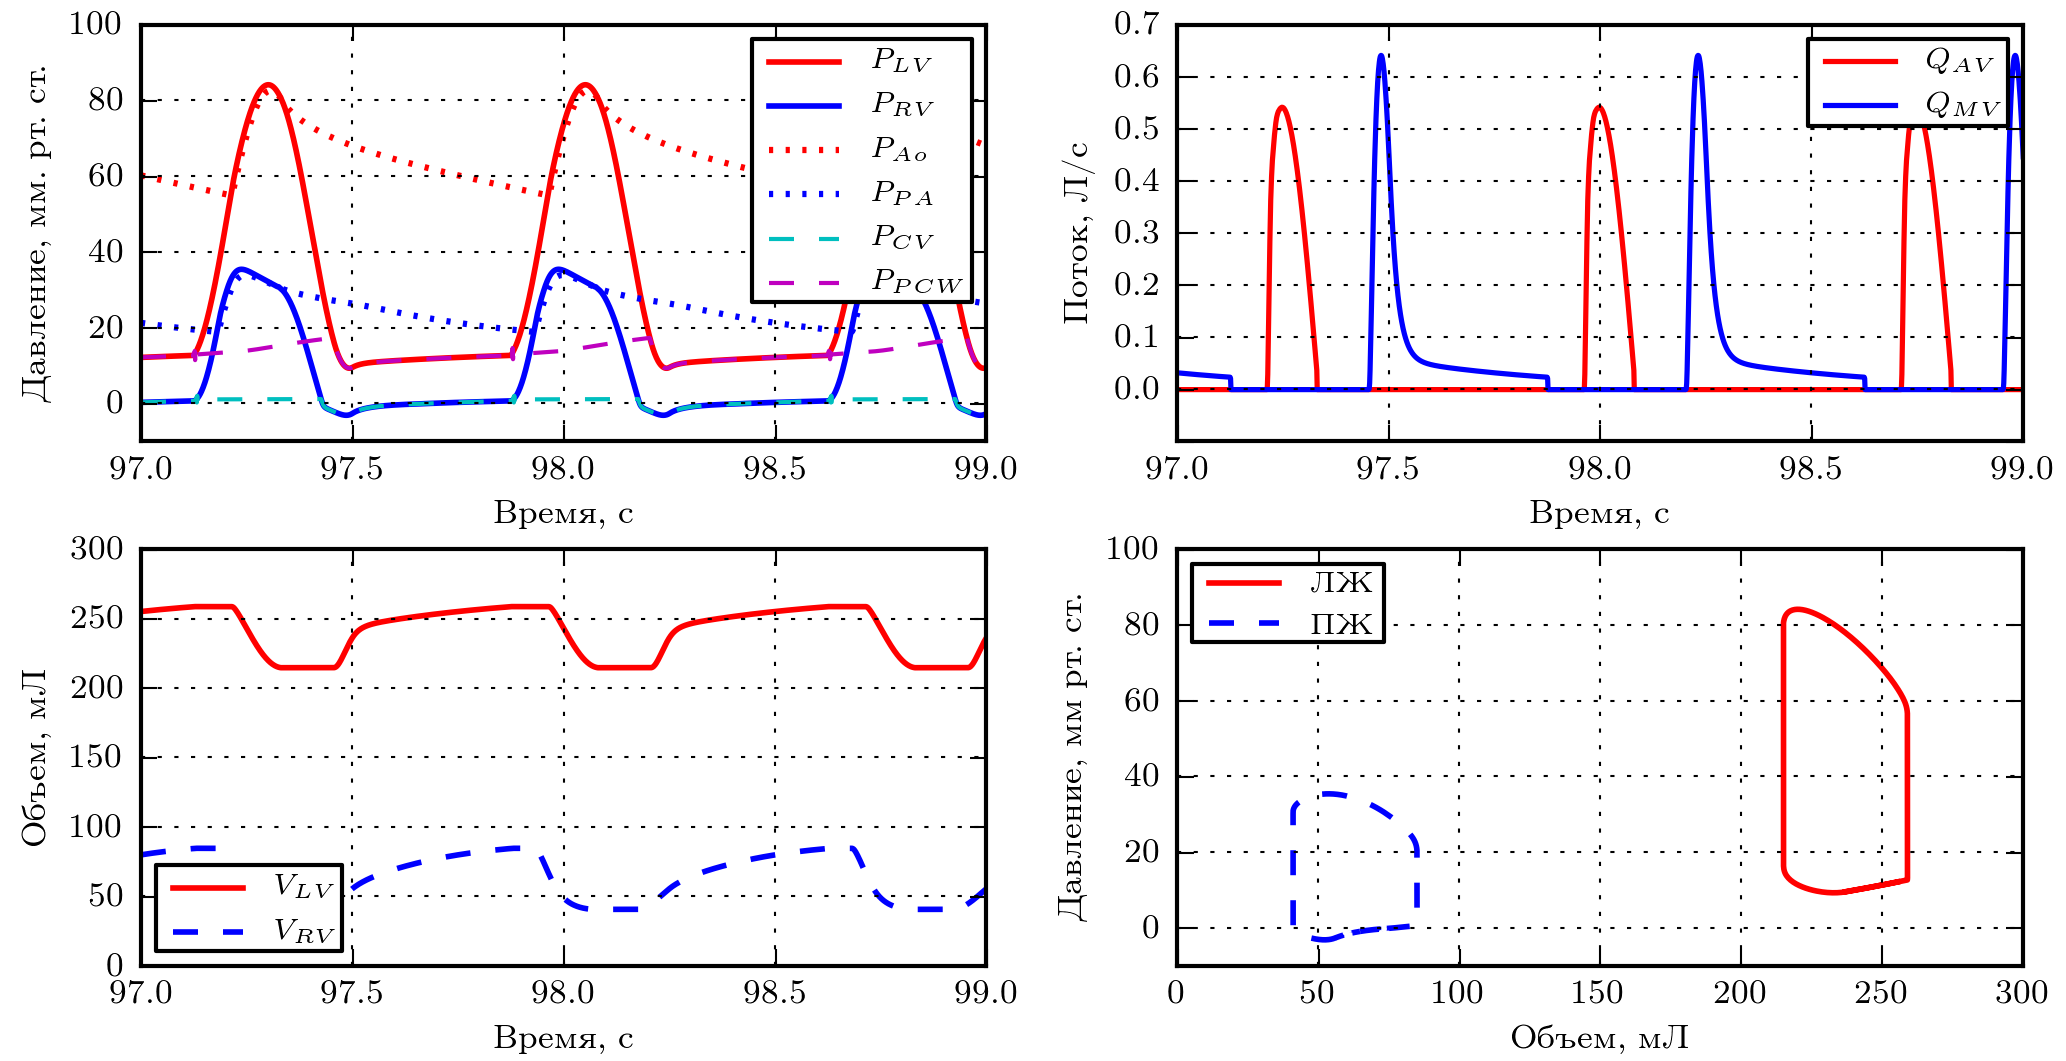
\includegraphics [scale=1.0] {../images/c2_cvs_hemodynamics}
  \caption{Гемодинамика в сердечно-сосудистой системе для случая сердечной недостаточности; $P_{LV}$ -- давление в левом желудочке сердца, $P_{RV}$ -- давление в правом желудочке сердца, $P_{Ao}$ -- давление в аорте, $P_{PA}$ -- давление в легочной артерии, $P_{CV}$ -- центральное венозное давление, $P_{PCW}$ -- давление заклинивания в легочных капиллярах, $V_{LV}$ и $V_{RV}$ -- объемы левого и правого желудочков сердца, $Q_{AV}$ и $Q_{MV}$ -- потоки через аортальный и митральный клапаны}
  \label{img:cvs_hemodynamics}
\end{figure}

Представленная гемодинамика характеризуется большим объемом левого желудочка сердца, а также меньшим систолическим давлением в аорте по сравнению с гемодинамикой в нормально функционирующей сердечно-сосудистой системе. Сдвиг контура давление-объем для левого желудочка сердца вправо вместе с уменьшением его площади согласуется с комбинированным типом сердечной недостаточности, описанным в разделе \ref{chapt1_history}.

% Рассмотренное состояние используется далее при исследовании взаимодействия насоса и сердечно-сосудистой системы.

Результаты разработки математической модели сердечно-сосудистой системы были представлены на 21-й Всероссийской конференции <<Микроэлектроника и информатика>> \cite{miee_2014}.

Разработанная математическая модель характеризуется широкими возможностями для модификации. Так, на основе рассмотренной математической модели разработаны модель сердечно-сосудистой системы педиатрических пациентов с врожденными пороками сердца \cite{mt4_2016} и модель сердечно-сосудистой системы для исследования механической поддержки кровообращения обоих желудочков сердца \cite{rgc_2016}.

Разработанная математическая модель реализована на языке программирования Python с использованием библиотеки NumPy. Программный код приведен в приложении \ref{list:cardiovascular_system_model}. 

\section*{Выводы по главе 2} 
\addcontentsline{toc}{section}{Выводы по главе 2}

В данной главе разработан алгоритм структурно-параметрической идентификации, который позволил построить математическую модель насоса на основе расходно-напорных характеристик роторного насоса крови HeartMate II. 

В ходе разработки модели идентификации реализована процедура оптимизации на основе алгоритма Левенберга-Марквардта, которая используется для определения коэффициентов математических моделей. 

Построенная в результате идентификации математическая модель имплантируемого роторного насоса крови позволяет оценивать расход насоса на основе данных о скорости вращения ротора, перепаде давления в насосе и вязкости жидкости в насосе.

В данной главе также разработана математическая модель сердечно-сосудистой системы с учетом имплантации роторного насоса крови. Разработанная математическая модель позволяет описать гемодинамику в сердечно-сосудистой системе в случае сердечной недостаточности. 
           % Глава 2
\chapter{Исследование взаимодействия имплантируемого роторного насоса крови и сердечно-сосудистой системы методами математического моделирования} \label{chapt3}

Цель данной главы заключается в исследовании взаимодействия имплантируемого роторного насоса крови и сердечно-сосудистой системы методами математического моделирования и последующем анализе результатов для повышения эффективности идентификации и управления имплантируемым роторным насосом крови в аппаратах вспомогательного кровообращения. 

Исследование взаимодействия выполнено с использованием математических моделей, разработанных во \ref{chapt2}-й главе.

%модели насоса, описываемой уравнением \eqref{eq:final_pump_model}, -- далее, модели идентификации.

% ----------------------------------------------------------------------------------------------------------------------------------------------------------------------------------------------------------------------------
% ----------------------------------------------------------------------------------------------------------------------------------------------------------------------------------------------------------------------------

%\section{Исследование взаимодействия математических моделей идентификации и сердечно-сосудистой системы}

%В данной части моделируется взаимодействие сердечно-сосудистой системы и имплантируемого роторного насоса крови с использованием математической модели насоса, описываемой уравнением \eqref{eq:final_pump_model}. 

Рассмотрен случай подключения входа насоса к левому желудочку сердца, выхода насоса -- к аорте, как показано на рисунке \ref{img:full_cvs}, при частоте сердечных сокращений 80 уд/мин.

В ходе моделирования получены расходно-напорные характеристики имплантируемого роторного насоса крови -- рисунок \ref{img:dynamic_hqs}. 

\begin{figure}[ht] 
  \center
  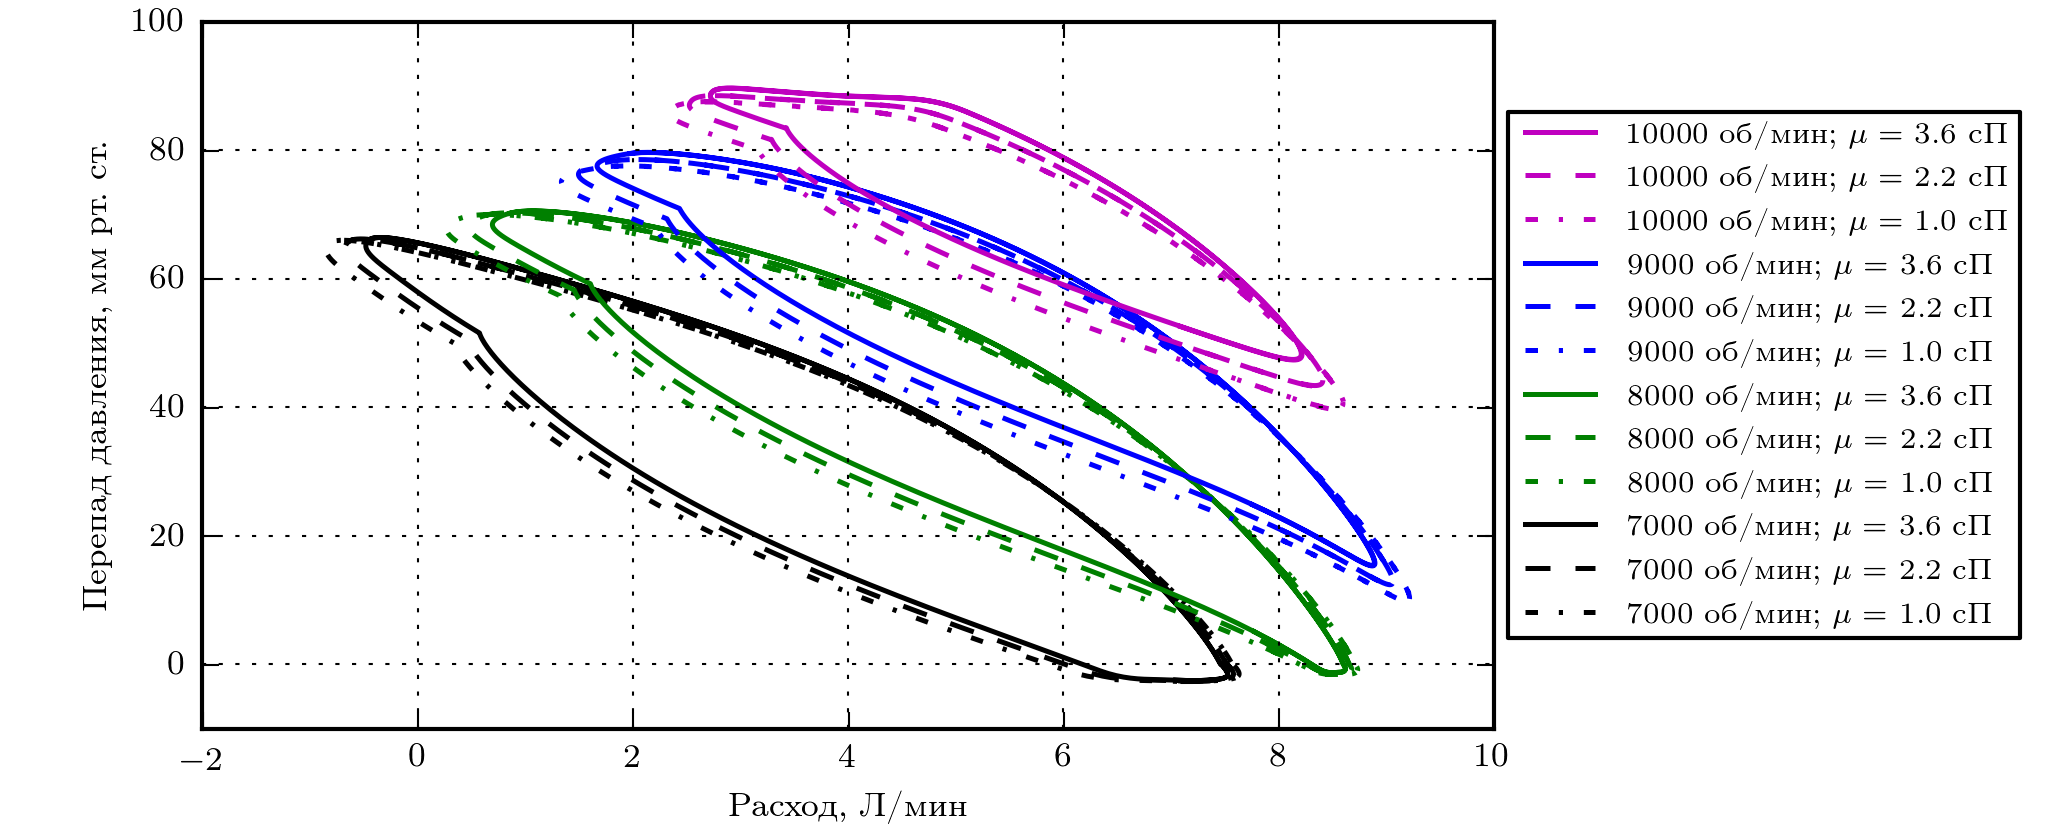
\includegraphics [scale=1.0] {../images/c2_dynamic_model_final}
  \caption{Динамические расходно-напорные характеристики роторного насоса крови при различных скоростях насоса $\omega$ (об/мин) и вязкости жидкости $\mu$ (сП) в диапазоне от 1,0 сП до 3,6 сП} 
  \label{img:dynamic_hqs}  
\end{figure}

Нелинейная форма расходно-напорных характеристик наблюдается в случае подключения насоса к биологическому сердцу или механизму -- источнику искусственных пульсаций, и обусловлена инерционными эффектами жидкости в насосе.
Полученный результат представлен в 2014 году на конференции <<Медицинская физика и инновации в медицине>> \cite{tkmf_2014} и согласуется с данными, опубликованными в литературе \cite{Moscato_2009, stanfield_vitro_2013, Pirbodaghi_2011,Thorsten_1996,Vollkron_2002,Pennings_2013,HQ_s_d_2015}.

Также исследована зависимость гемодинамических показателей от скорости вращения ротора насоса -- рисунок \ref{img:cvs_pump_hemodynamics}, где черной пунктирной отмечена исходная величина гемодинамического показателя в сердечно-сосудистой системе без насоса. Скорость насоса изменялась в диапазоне от 7200 об/мин до 9800 об/мин с шагом 200 об/мин. Красным квадратным маркером отмечено значение гемодинамического показателя при скорости насоса, при которой поток через аортальный клапан $Q_{AV}$ уменьшается до нуля с увеличением скорости насоса.

\begin{figure}[ht] 
  \center
  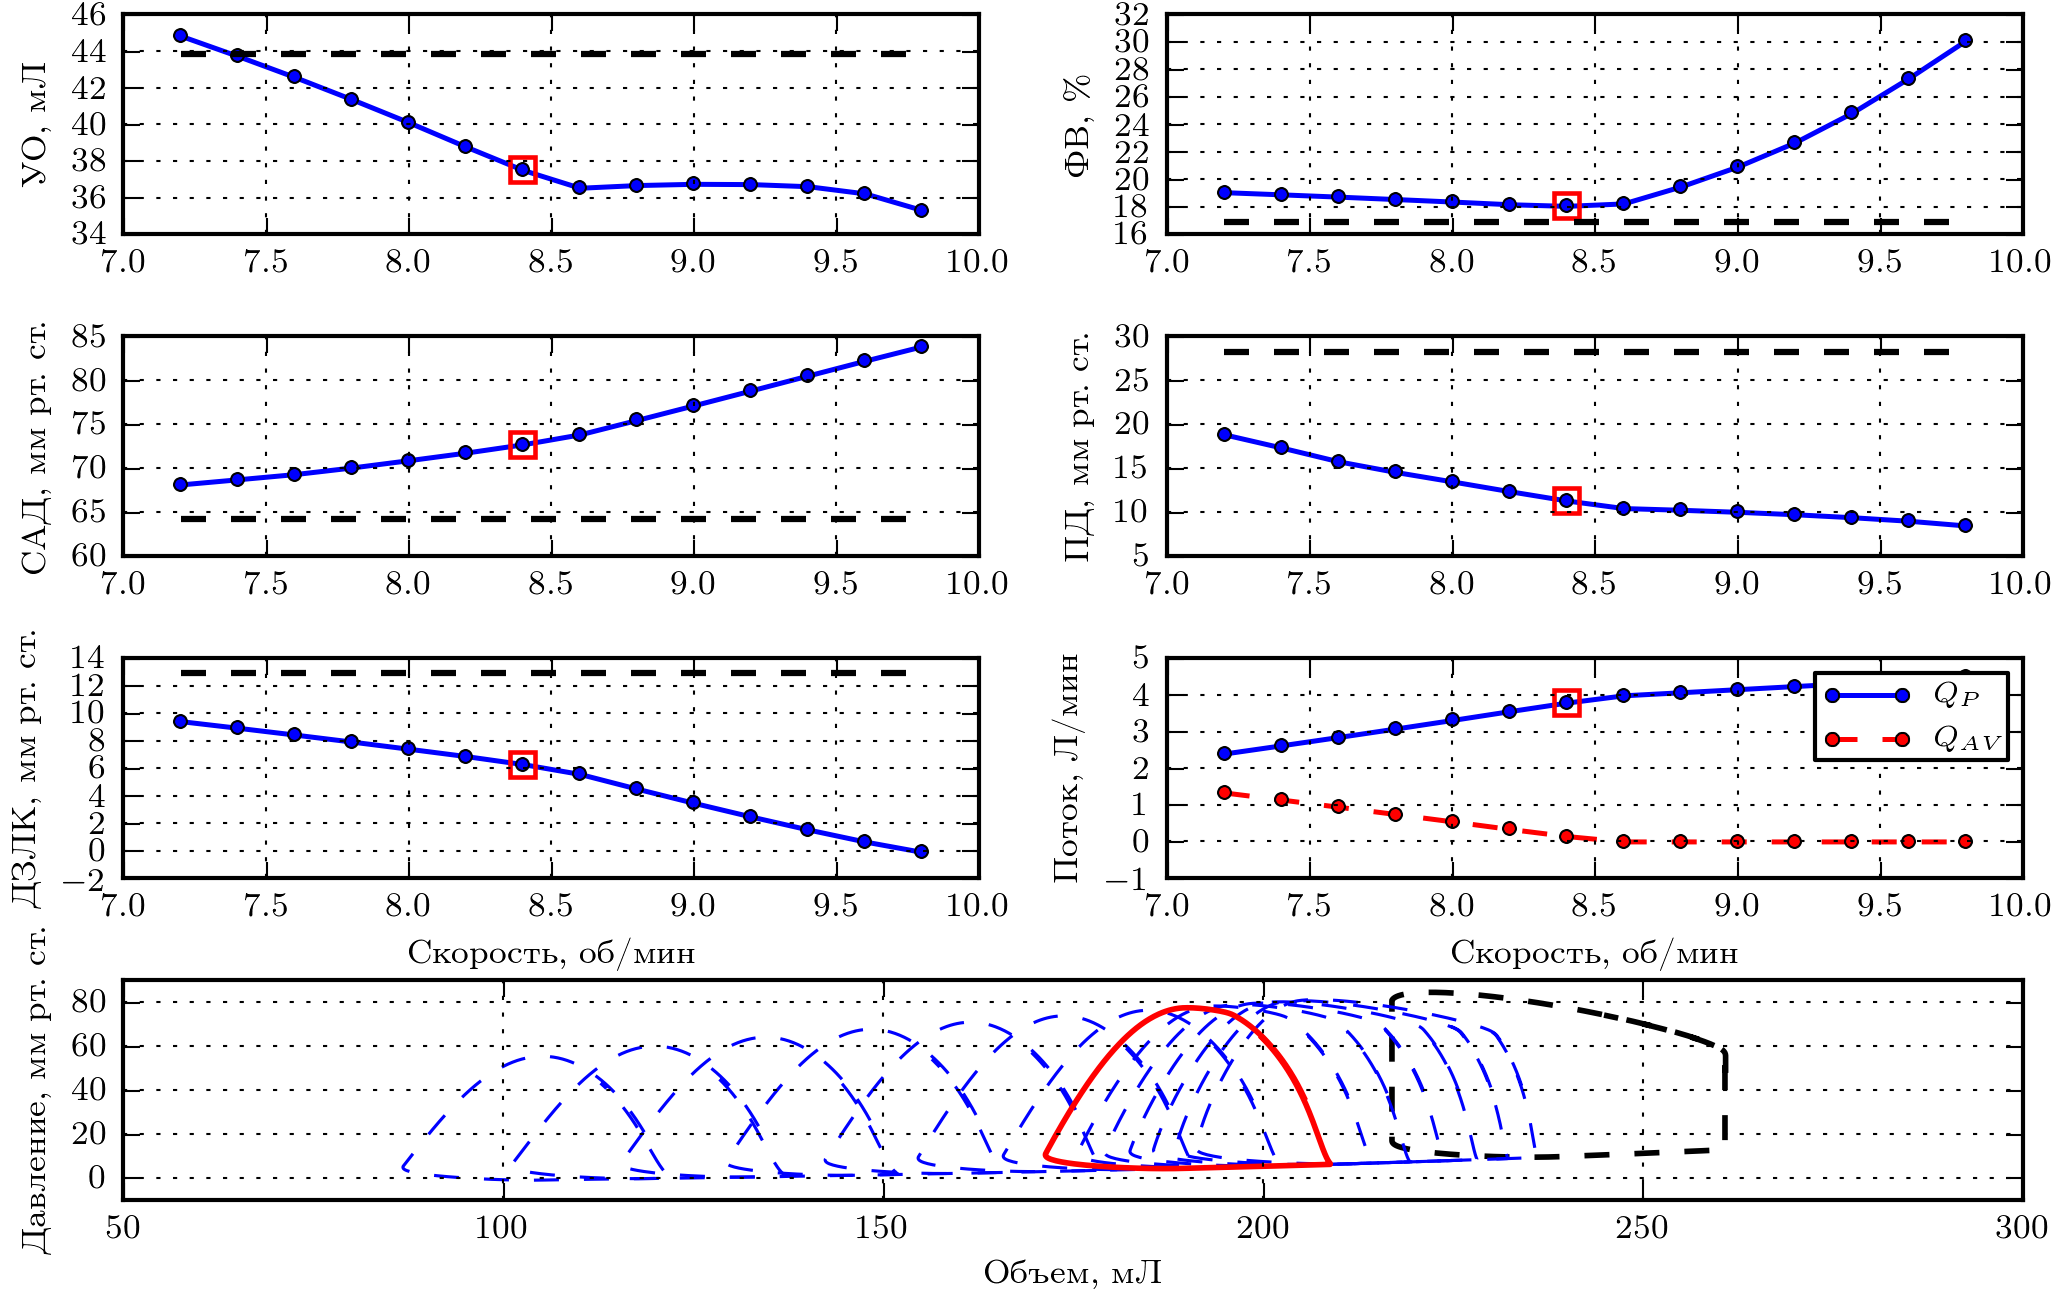
\includegraphics [scale=1.0] {../images/c2_cvs_pump_hemodynamics}
  \caption{Изменение гемодинамических показателей и контуров давление-объем левого желудочка сердца при различных скоростях насоса; УО -- ударный объем, ФВ -- фракция выброса, $P_{PCW}$ -- давление заклинивания в легочных капиллярах, ПД -- пульсовое давление, $Q_P$ -- расход насоса, $Q_{AV}$ -- поток через аортальный клапан} \label{img:cvs_pump_hemodynamics}
\end{figure}

Сравнительное исследование имплантируемых роторных насосов крови по влиянию на сердечно-сосудистую систему методами математического моделирования было представлено на 37-й международной конференции сообщества IEEE по инженерии в медицине и биологии \cite{embc_2015_2}. 

Результаты исследования взаимодействия имплантируемого роторного насоса крови с сердечно-сосудистой системой методами математического моделирования с акцентом на кровообращение в малом круге кровообращения и функцию правого желудочка сердца были опубликованы в журнале <<Медицинская техника>> \cite{mt4_2014} и представлены на международной конференции \cite{rgc_2014}.

Результаты исследования взаимодействия имплантируемых роторных насосов крови с сердечно-сосудистой системой методами математического моделирования в случае механической поддержки кровообращения обоих желудочков сердца были подготовлены и опубликованы в 2017 году в журнале <<Медицинская техника>> \cite{mt1_2017}, а также представлены на международной конференции ФРЭМЭ -- 2014 \cite{freme_2014}.   

\section{Определение режимов работы имплантируемого роторного насоса крови} \label{sect3_2}

В ходе моделирования получены зависимости, описывающие изменение гемодинамических показателей при изменении скорости насоса -- рисунок \ref{img:pumping_states_general}. 

\begin{figure}[ht] 
  \center
  \noindent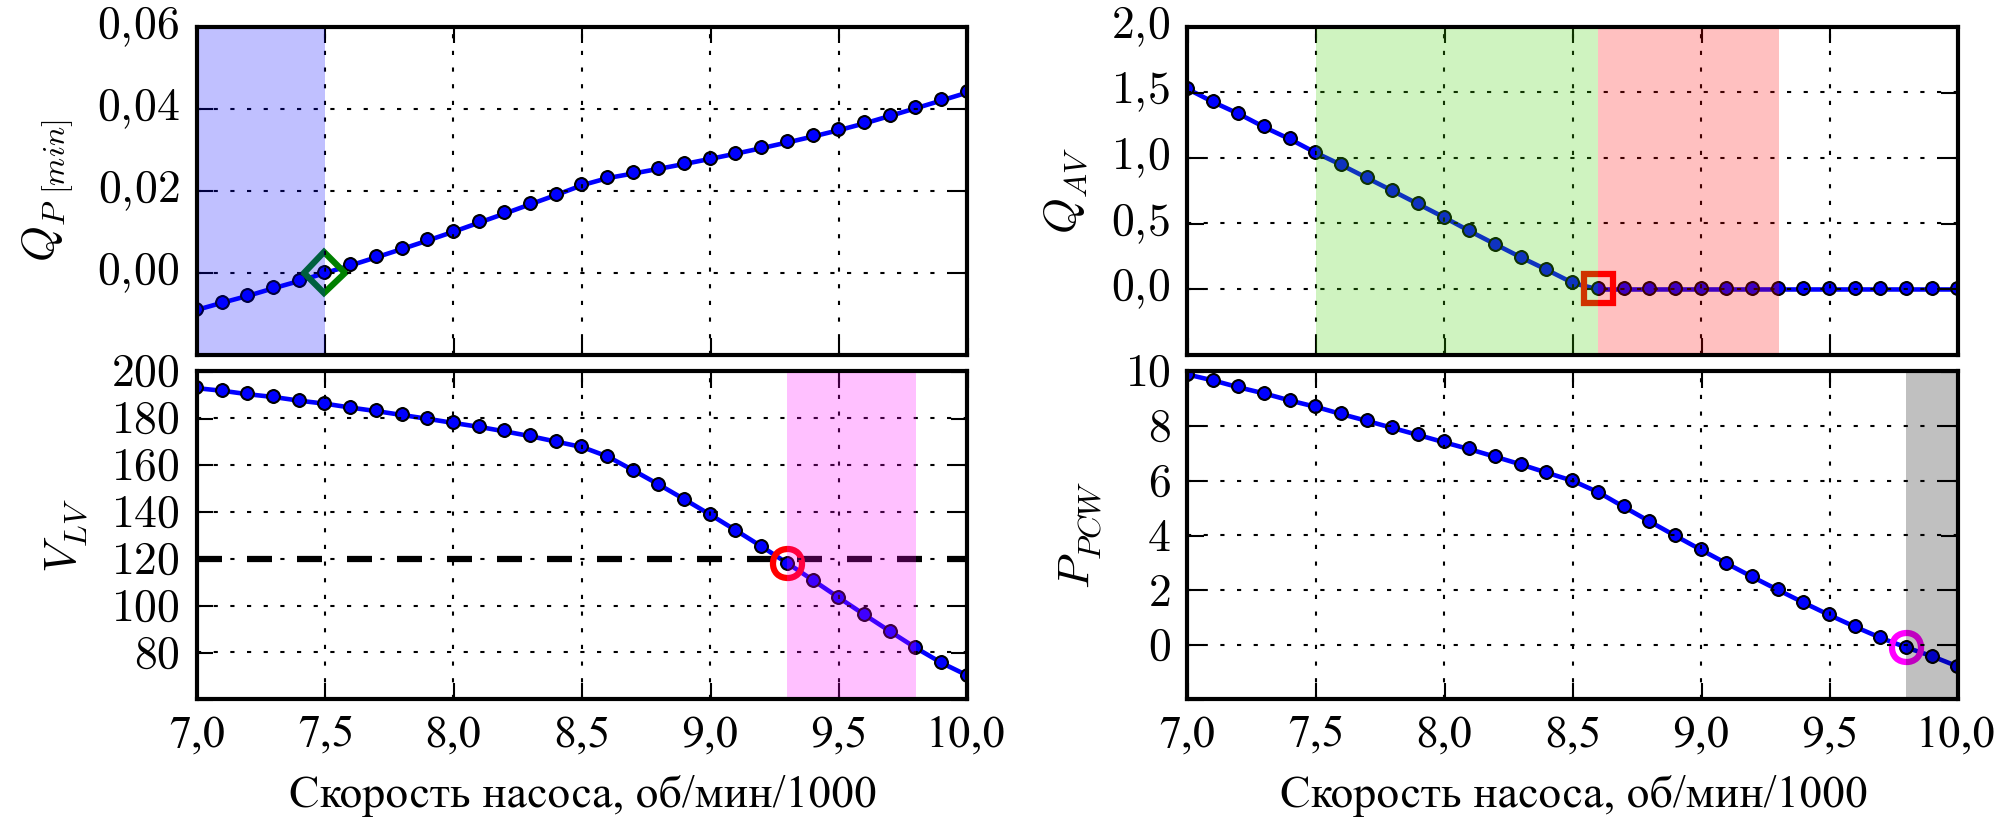
\includegraphics [scale=1.0] {../images/c3_pumping_states_dis}
  \caption{Гемодинамические зависимости, полученные на математической модели сердечно-сосудистой системы;  $Q_{P[min]}$ -- минимальный расход насоса (л/с), $Q_{AV}$ -- поток через аортальный клапан (л/мин), $V_{LV}$ -- конечно-систолический объем левого желудочка (мл), $P_{PCW}$ -- давление заклинивания в легочных капиллярах (мм рт. ст.)} 
  \label{img:pumping_states_general}  
\end{figure}

Полученные зависимости позволяют определить режимы работы насоса -- состояния в сердечно-сосудистой системе, обусловленные спецификой работы имплантируемого роторного насоса крови \cite{ayre_identifying_2001, Karantonis_2006, Karantonis_2007, karantonis2007classification, Ng_2013}. В данной работе рассматриваются следующие режимы: обратное течение через насос ($P_{BF}$), частичная разгрузка ($P_{PA}$) и полная разгрузка желудочка сердца ($P_{FA}$), частичный коллапс ($P_{PVC}$) и полный коллапс желудочка сердца ($P_{FVC}$). 

Так, на рисунке \ref{img:pumping_states_general} синим цветом отмечен режим обратного течения, определенный из зависимости $Q_{P[min]}$ от скорости насоса и обозначающий отрицательный поток через насос во время сердечного цикла. Переход из режима обратного течения в режим частичной разгрузки желудочка сердца отмечен зеленым маркером. 

Уменьшение $Q_{AV}$ до нуля с увеличением скорости насоса, отмеченное красным маркером, соответствует полностью закрытому состоянию АК и работе насоса в режиме  полной разгрузки желудочка сердца. Аналогичным образом обозначены переходы между режимами работы $P_{FA}$ и $P_{PVC}$ на зависимости $V_{LV}$ от скорости насоса, между режимами $P_{PVC}$ и $P_{FVC}$ на зависимости $P_{PCW}$ от скорости насоса.   

% Увеличение скорости насоса приводит к уменьшению конечно-систолического объема ЛЖ до исходного значения, соответствующего нулевому давлению в желудочке, что отмечено красным круглым маркером на зависимости $V_{LV}$ от скорости насоса и соответствует переходу в режим $P_{PVC}$. Переход из режима частичного коллапса в режим $P_{FVC}$ отмечен круглым фиолетовым маркером на зависимости $P_{PCW}$ от скорости насоса. 

В ходе анализа результатов моделирования на основе математической модели идентификации предложен метод определения режимов работы насоса, который заключается в оценке изменений в динамике течения жидкости через насос. Анализ и оценка изменений в динамике течения осуществляется с помощью частных производных по зависимым переменным $Q$ и $\omega$, которые найдены из математической модели, описываемой уравнением \eqref{eq:final_pump_model} \cite{mt6_2014_main, rgc_2015}.

По результатам исследования производных на математической модели сердечно-сосудистой системы установлено, что каждая  производная характеризуется определенной динамикой за время одного сердечного цикла. В то же время изменение скорости насоса может приводить к изменению динамики производной. Примеры временных диаграмм производных $dQ/dt$, $d^2Q/dt^2$, $d^3Q/dt^3$, $dQ/dt~dQ/d\omega$, $dQ/dt~d^2Q/d\omega^2$ длительностью два сердечных цикла при различных скоростях насоса представлены на рисунке \ref{img:derivatives_waveform}.

\begin{figure}[ht] 
  \center
  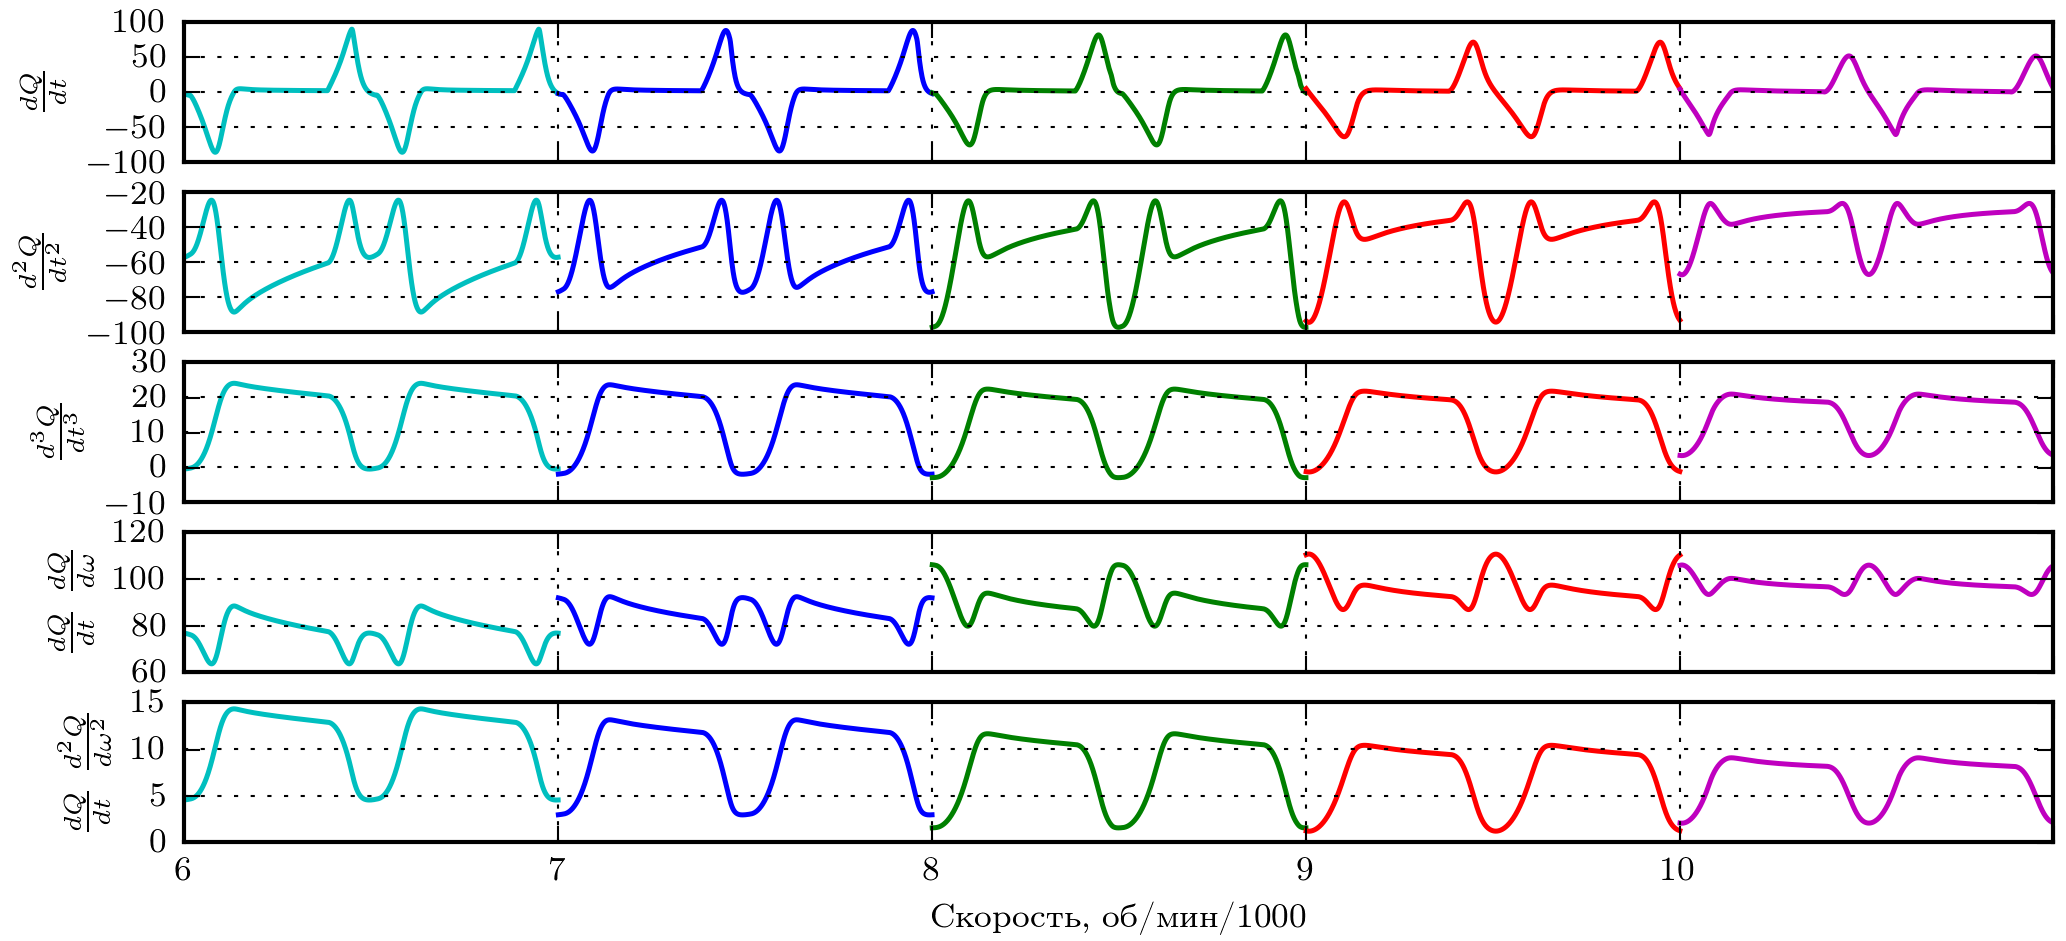
\includegraphics [scale=1.0] {../images/c3_derivatives_waveform}
  \caption{Временные диаграммы производных в диапазоне скоростей насоса от 6000 об/мин до 10000 об/мин} 
  \label{img:derivatives_waveform}  
\end{figure}

Сравнительный анализ гемодинамических зависимостей, представленных  на рисунке \ref{img:pumping_states_general}, и производных, найденных из модели идентификации, позволил установить корреляцию между режимами работы насоса и изменениями производных. Пример корреляции между потоком через аортальный клапан и производной $dQ/dt~dQ/d\mu$ представлен на рисунке \ref{img:av_derivative_waveform}. В данном случае нулевому потоку через клапан при увеличении скорости насоса соответствует увеличение минимального значения производной за один сердечный цикл.

\begin{figure}[ht] 
  \center
  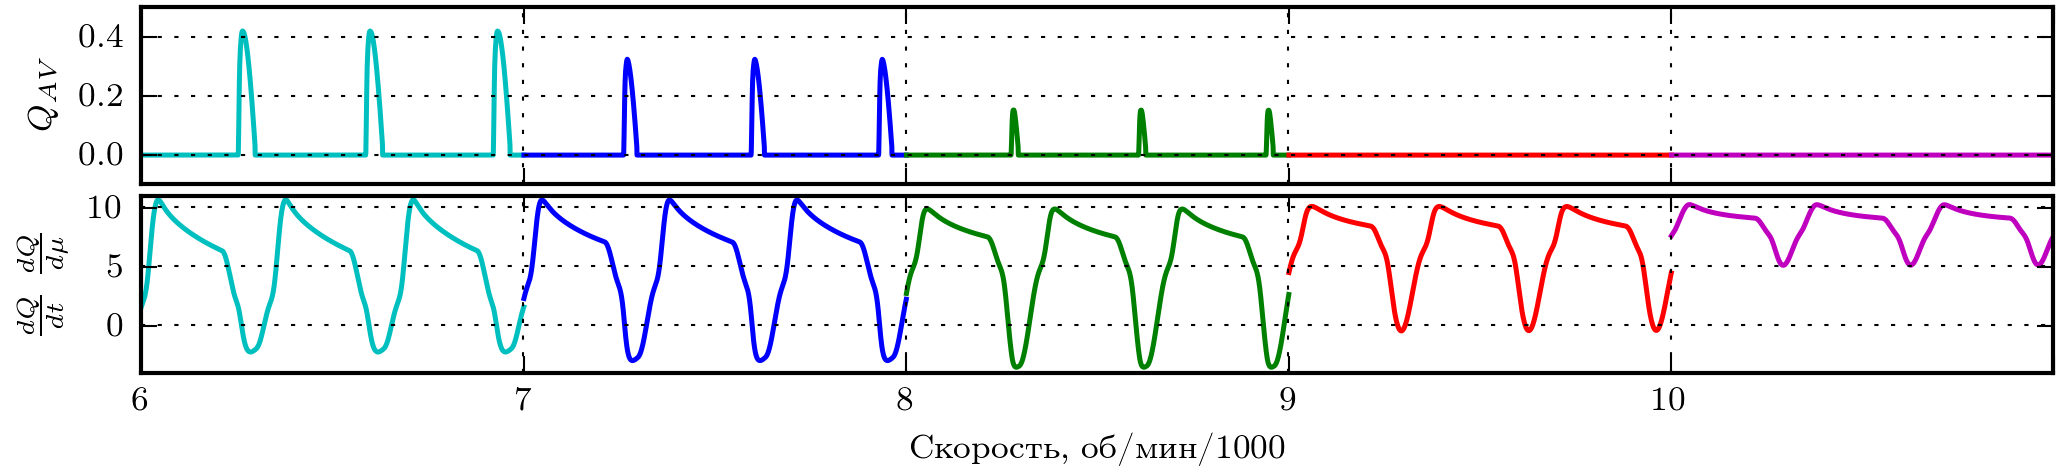
\includegraphics [scale=1.0] {../images/c3_example_correlation}
  \caption{Временная диаграмма потока через аортальный клапана $Q_{AV}$ (л/с) и производной $dQ/dt~dQ/d\mu$ в диапазоне скоростей насоса от 6000 об/мин до 10000 об/мин} 
  \label{img:av_derivative_waveform}  
\end{figure}

Для описания изменений в динамике производных, которые коррелируют с режимами работы насоса, введены индексы. Значение каждого индекса представляет максимальное ($\max$) или минимальное ($\min$) или комбинацию максимального и минимального значения производной за время одного сердечного цикла \cite{mt6_2014_main, rgc_2015}. 

Список индексов для определения режимов работы насоса представлен в таблице \ref{tbl:pump_model_derivatives_indices}. 

\begin{table} [htbp]%
    \centering
	\caption{Индексы для определения режимов работы насоса}%
	\label{tbl:pump_model_derivatives_indices}% label всегда желательно идти после caption
    \renewcommand{\arraystretch}{1.5} 
	\begin{tabular}{@{}@{\extracolsep{20pt}}llll@{}} 
        \toprule     %%% верхняя линейка
    	Режим работы & Индекс \\
        \midrule %%% тонкий разделитель. Отделяет названия столбцов. Обязателен по ГОСТ 2.105 пункт 4.4.5 
    	$P_{BF}/P_{PA}$ & $\begin{multlined}S_{BF} = \max\frac{d^2Q}{dt^2}\frac{dQ}{d\mu} - \min \frac{d^2Q}{dt^2}\frac{dQ}{d\mu} \end{multlined}$ \\
		 & \\
 		$P_{PA}/P_{FA}$ & $\begin{multlined}S_{AV1} = -2\min\frac{dQ}{dt}\frac{dQ}{d\mu} / \left( \max\frac{dQ}{dt}\frac{dQ}{d\mu} - \min\frac{dQ}{dt}\frac{dQ}{d\mu} \right)\end{multlined}$ \\
		 & \\
 		$P_{PA}/P_{FA}$ & $\begin{multlined}S_{AV2} = \max\frac{d^2Q}{dt^2}\frac{dQ}{d\omega} / \left( \max\frac{d^2Q}{dt^2}\frac{dQ}{d\omega} - \min\frac{d^2Q}{dt^2}\frac{dQ}{d\omega} \right)\end{multlined}$ \\
		 & \\
 		$P_{FA}/P_{PVC}$ & $\begin{multlined}S_{VC1} = \max \frac{dQ}{dt}\frac{dQ}{d\omega}\end{multlined}$ \\
		 & \\
 		$P_{PVC}/P_{FVC}$ & $\begin{multlined}S_{VC2} = -2\min \frac{dQ}{dt} / \left( \max\frac{dQ}{dt} - \min\frac{dQ}{dt} \right)\end{multlined}$ \\
        \bottomrule %%% нижняя линейка
	\end{tabular}%
\end{table}

\section*{Результаты определения режимов работы роторного насоса крови на математической модели сердечно-сосудистой системы} \label{sect3_3}

Данные результаты получены на математической модели сердечно-сосудистой системы в случае подключения роторного насоса крови к левому желудочку сердца и аорте аналогично рисунку \ref{img:full_cvs}. Исходная частота сердечных сокращений равнялась 80 уд/мин, исходное значение объема левого желудочка, соответствующее нулевому давлению в желудочке сердца, равнялось 120 мл. Сократительная способность левого желудочка сердца изменялась на $\pm$10\% посредством задания параметра $C_V$ в модели сердца равным 0,45 и 0,55. 

\subsection*{Определение режима обратного течения через насос}

На рисунке \ref{img:pumping_states_bf_36} представлена зависимость индекса $S_{BF}$ от скорости насоса при изменении сократимости ЛЖ и частоты сердечных сокращений и параметре $\mu$ в математической модели идентификации равным 3,6 сП. Зеленым ромбовидным маркером обозначен переход между режимами $P_{BF}$ и $P_{PA}$, определенный из зависимости $Q_{P[min]}$ от скорости насоса.

\begin{figure}[ht] 
  \center
  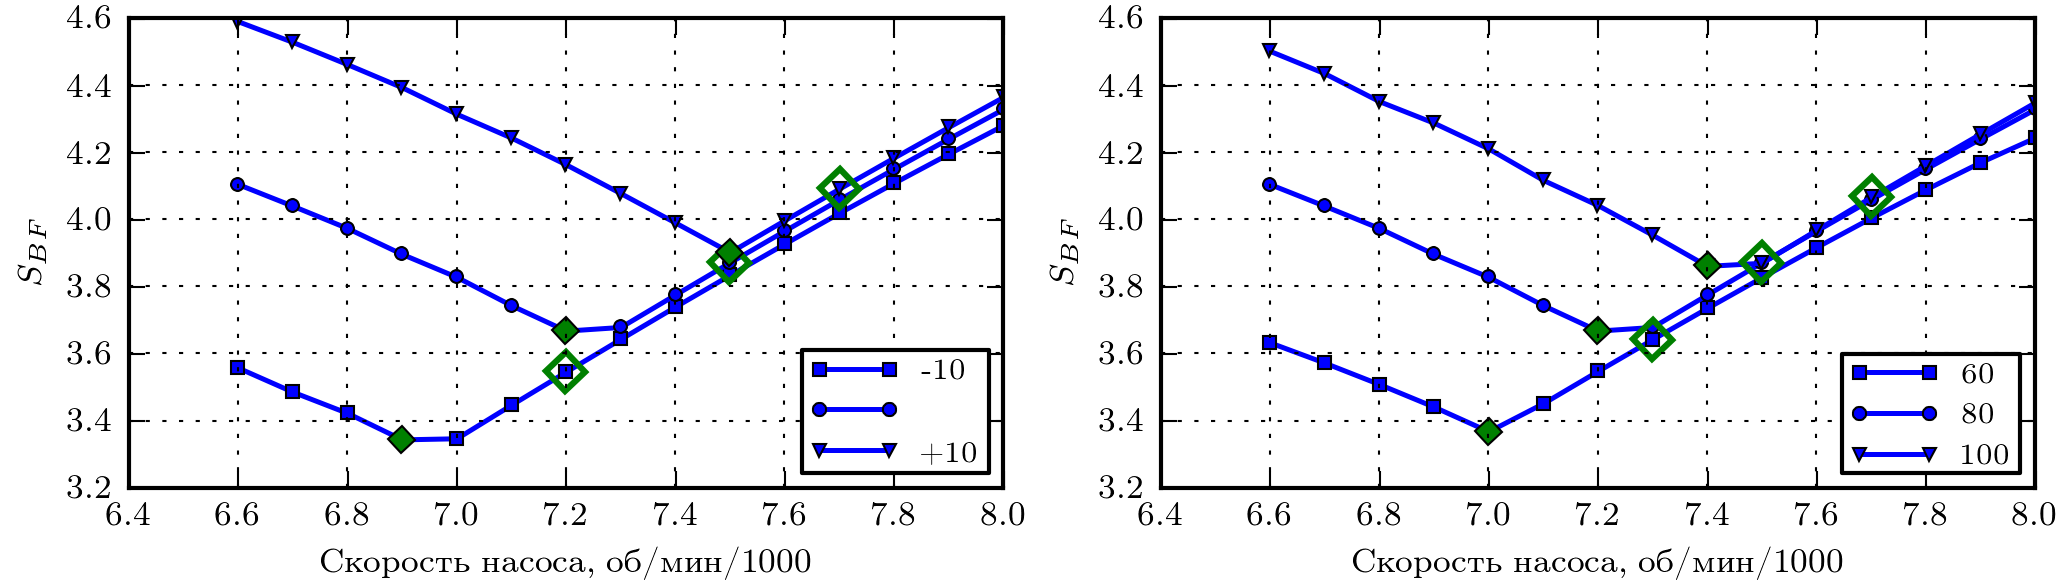
\includegraphics [scale=1.0] {../images/c3_bf_36}
  \caption{Зависимость индекса $S_{BF}$ от скорости насоса при изменении сократимости левого желудочка сердца, \% (слева) и частоты сердечных сокращений, уд/мин (справа) и параметре $\mu =$ 3,6 сП} 
  \label{img:pumping_states_bf_36}  
\end{figure}

Аналогичным образом был исследован индекс $S_{BF}$ при параметре $\mu =$ 2,2 сП. Результаты исследования представлены на рисунке \ref{img:pumping_states_bf_22}.

\begin{figure}[ht] 
  \center
  \includegraphics [scale=1.0] {../images/c3_bf_22}
  \caption{Зависимость индекса $S_{BF}$ от скорости насоса при изменении сократимости левого желудочка сердца, \% (слева) и частоты сердечных сокращений, уд/мин (справа) и параметре $\mu =$ 2,2 сП} 
  \label{img:pumping_states_bf_22}  
\end{figure}

Уменьшению $S_{BF}$ при увеличении скорости насоса соответствует режим обратного течения через насос. Изменению в динамике индекса при увеличении скорости насоса соответствует переход в режим $P_{PA}$, который отмечен зеленым ромбовидным маркером. 

Для вычисления точности определения перехода между режимами работы насоса была предложена следующая формула:

\begin{equation}
	\label{eq:ps_identification_accuracy}
	\delta(PS) = \left(1 - \frac{\lvert \omega_t - \omega_m \rvert}{\omega_{max} - \omega_{min}} \right) \cdot 100\%,
\end{equation}

\noindent где $\omega_t$ -- практическое значение скорости насоса, при которой происходит переход между режимами работы, определенное из гемодинамической зависимости, $\omega_m$ -- расчетное значение скорости насоса, при которой происходит переход между режимами работы, определенное с помощью производной, $\omega_{max}$ и $\omega_{min}$ -- верхняя и нижняя граница скорости вращения ротора насоса. 

Представленные зависимости позволяют определить нижнюю границу скорости $\omega_{min}$ -- 7400 об/мин. Данное значение рассчитано как разность скорости, при которой происходит переход между режимами $P_{BF}$ и $P_{PA}$ в начальных условиях ($C_V =$ 0,5, $\mu =$ 3,6 сП и ЧСС 80 уд/мин) -- 7500 об/мин, и шага по скорости (100 об/мин).

\subsection*{Определение режимов частичной разгрузки и полной разгрузки желудочка сердца}

На рисунке \ref{img:pumping_states_pa_fa_36} представлена зависимость индексов $S_{AV1}$ и $S_{AV2}$ от скорости насоса при изменении сократимости ЛЖ и частоты сердечных сокращений и параметре $\mu =$ 3,6 сП. 

\begin{figure}[!ht] 
  \center
  \includegraphics [scale=1.0] {../images/c3_pa_fa_36}
  \caption{Зависимость индексов $S_{AV1}$ и $S_{AV2}$ от скорости насоса при изменении сократимости левого желудочка сердца, \% (слева) и частоты сердечных сокращений, уд/мин (справа) и параметре $\mu =$ 3,6 сП} 
  \label{img:pumping_states_pa_fa_36}  
\end{figure}

Аналогичным образом были исследованы индексы $S_{AV1}$ и $S_{AV2}$ при задании параметра $\mu$ равным 2,2 сП. Результаты исследования представлены на рисунке \ref{img:pumping_states_pa_fa_22}.

\begin{figure}[!ht] 
  \center
  \includegraphics [scale=1.0] {../images/c3_pa_fa_22}
  \caption{Зависимость индексов $S_{AV1}$ и $S_{AV2}$ от скорости насоса при изменении сократимости левого желудочка сердца, \% (слева) и частоты сердечных сокращений, уд/мин (справа) и параметре $\mu =$ 2,2 сП} 
  \label{img:pumping_states_pa_fa_22}  
\end{figure}

Большим красным квадратным маркером обозначен переход из режима $P_{PA}$ в режим $P_{FA}$, определенный из зависимости $Q_{AV}$ от скорости насоса. Таким образом, увеличению обоих индексов при увеличении скорости насоса соответствует режим частичной разгрузки желудочка сердца. 

Изменение в динамике индексов $S_{AV}$, отмеченное малым квадратным маркером, обозначает полностью закрытое состояние АК и переход в режим полной разгрузки желудочка сердца. %Изменение в динамике $S_{AV1}$ определяет переход к режиму полной разгрузки раньше $S_{AV2}$, пренебрегая незначительным (менее 0,1 л/мин) потоком через АК.

\subsection*{Определение режимов частичного коллапса и полного коллапса желудочка сердца}

На рисунке \ref{img:pumping_states_pvc_fvc_36} представлена зависимость индексов $S_{VC1}$ и $S_{VC2}$ от скорости насоса при изменении сократимости ЛЖ и частоты сердечных сокращений и параметре $\mu =$ 3,6 сП. Режимы частичного коллапса и полного коллапса желудочка обозначены круглыми маркерами красного и фиолетового цветов: первому соответствуют отрицательное конечно-систолическое давление в левом желудочке сердца (определено из зависимости $V_{LV}$ от скорости насоса), второму -- отрицательное давление заклинивания в легочных капиллярах (определено из зависимости $P_{PCW}$ от скорости насоса). 

\begin{figure}[ht] 
  \center
  \includegraphics [scale=1.0] {../images/c3_pvc_fvc_36}
  \caption{Зависимость индексов $S_{VC1}$ и $S_{VC2}$ от скорости насоса при изменении сократимости левого желудочка сердца, \% (слева) и частоты сердечных сокращений, уд/мин (справа) и параметре $\mu =$ 3,6 сП} 
  \label{img:pumping_states_pvc_fvc_36}  
\end{figure}

Таким образом, изменение в динамике индекса $S_{VC1}$ при увеличении скорости насоса позволяет определить переход в режим частичного коллапса желудочка сердца. Аналогичным образом изменение в динамике индекса $S_{VC2}$, отмеченное круглым фиолетовым маркером, позволяет определить переход в режим полного коллапса желудочка сердца. 

Представленные зависимости также позволяют определить верхнюю границу скорости $\omega_{min}$ -- 9900 об/мин. Данное значение рассчитано как сумма скорости, при которой происходит переход между режимами $P_{PVC}$ и $P_{FVC}$ в начальных условиях ($C_V =$ 0,5, $\mu =$ 3,6 сП и ЧСС 80 уд/мин) -- 9800 об/мин, и шага по скорости (100 об/мин).

Аналогичным образом были исследованы индексы $S_{VC1}$ и $S_{VC2}$ при задании параметра $\mu$ равным 2,2 сП. Результаты исследования представлены на рисунке \ref{img:pumping_states_pvc_fvc_22}.

\begin{figure}[ht] 
  \center
  \includegraphics [scale=1.0] {../images/c3_pvc_fvc_22}
  \caption{Зависимость индексов $S_{VC1}$ и $S_{VC2}$ от скорости насоса при изменении сократимости левого желудочка сердца, \% (слева) и частоты сердечных сокращений, уд/мин (справа) и параметре $\mu =$ 2,2 сП} 
  \label{img:pumping_states_pvc_fvc_22}  
\end{figure}

Результаты расчета точности определения переходов между режимами работы насоса при изменении сократимости левого желудочка сердца и частоты сердечных сокращений и параметре $\mu$ в модели идентификации равном 3,6 сП представлены в таблице \ref{tbl:ps_identification_accuracy_model}, при параметре $\mu =$ 2,2 сП -- в таблице \ref{tbl:ps_identification_accuracy_model_2_2}.

%Результаты расчета точности при трех значениях параметра $\mu$ математической модели насоса представлены в таблице \ref{tbl:ps_identification_accuracy_model}. Приведенные значения являются средними в широком диапазоне сократимостей левого желудочка сердца и частот сердечных сокращений.

% \begin{table} [htbp]%
%     \centering
% 	\caption{Точность определения переходов между режимами работы насоса ($\delta$, \%)}%
% 	\label{tbl:ps_identification_accuracy_model}%
%     \renewcommand{\arraystretch}{1.5} 
% 	\begin{tabular}{@{}@{\extracolsep{20pt}}llll@{}} 
% 	\toprule
% 	& $\mu = $ 3,6 сП & $\mu = $ 2,2 сП & $\mu = $ 1,0 сП\\
% 	\midrule
% 	$\delta(P_{BF}/P_{PA})$			& 88,7		&	87,5 & 85,4\\
% 	$\delta(P_{PA}/P_{FA})$				& 98,0		& 97,9	& 97,6\\
% 	$\delta(P_{FA}/P_{PVC})$			& 90,6		& 94,5	& 94,4\\
% 	$\delta(P_{PVC}/P_{FVC})$		& 82,7		& 83,4	& 82,6\\
%     \bottomrule 
% 	\end{tabular}%
% \end{table}

\begin{table} [htbp]%
    \centering
	\caption{Точность определения режимов работы насоса (\%) при параметре $\mu =$ 3,6 сП}%
	\label{tbl:ps_identification_accuracy_model}% label всегда желательно идти после caption
    \renewcommand{\arraystretch}{1.5} 
	\begin{tabular}{@{}@{\extracolsep{20pt}}llll@{}} 
	\toprule
	& Сократимость & ЧСС & Среднее\\
	\midrule
	$P_{BF}/P_{PA}$					& 89,3		&	88,0		& 88,6\\
	$P_{PA}/P_{FA}$	& 98,0		& 98,0		& 98,0\\
	$P_{FA}/P_{PVC}$				& 92,0		& 89,3		& 90,6\\
	$P_{PVC}/P_{FVC}$				& 84,0		& 81,3		& 82,6\\
    \bottomrule 
	\end{tabular}%
\end{table}

\begin{table} [htbp]%
    \centering
	\caption{Точность определения режимов работы насоса (\%) при параметре $\mu =$ 2,2 сП}%
	\label{tbl:ps_identification_accuracy_model_2_2}% label всегда желательно идти после caption
    \renewcommand{\arraystretch}{1.5} 
	\begin{tabular}{@{}@{\extracolsep{20pt}}llll@{}} 
	\toprule
	& Сократимость & ЧСС & Среднее\\
	\midrule
	$P_{BF}/P_{PA}$					& 88,0		&	88,0		& 88,0\\
	$P_{PA}/P_{FA}$	& 98,0		& 98,0		& 98,0\\
	$P_{FA}/P_{PVC}$				& 96,0		& 93,3		& 94,7\\
	$P_{PVC}/P_{FVC}$				& 84,0		& 82,7		& 83,4\\
    \bottomrule 
	\end{tabular}%
\end{table}

Результаты данного исследования были опубликованы в конце 2014 года в журнале <<Медицинская техника>> \cite{mt6_2014_main}.

\newpage
\section{Управление имплантируемым роторным насосом крови}

На основе полученных результатов разработан способ управления имплантируемым роторным насосом крови с использованием скорости вращения ротора в качестве управляемой переменной. Цель управления заключается в  поддержании заданного уровня расхода насоса и предотвращении следующих нежелательных режимов работы насоса: обратное течение через насос, полная разгрузка желудочка сердца и коллапс желудочка сердца \cite{asaio_2015, embc_2015_1, miee_2016}.

Разработанный способ управления представлен в виде системы управления скоростью РНК на рисунке \ref{img:control_algorithm}. 

\begin{figure}[ht] 
  \center
  \includegraphics [scale=1.7] {../images/c3_control_algorithm}
  \caption{Обобщенная структура системы управления скоростью роторного насоса крови} 
  \label{img:control_algorithm}  
\end{figure}

Основным элементом системы является \textit{оценочный блок}, предназначенный для оценки расхода насоса и определения текущего режима работы насоса с использованием модели идентификации, описываемой уравнением \eqref{eq:final_pump_model}. 

Мгновенный расход насоса $Q(t)$ рассчитывается на основе данных о скорости вращения ротора $\omega$ (об/мин), перепаде давления в насосе $H$ (мм рт. ст.) и параметре $\mu$ (сП), который характеризует вязкость жидкости и задается в \textit{блоке электронного управления}.

Расход насоса $Q_A$ (л/мин) -- объем крови, перекачиваемый насосом за произвольное количество сердечных циклов. Расход насоса $Q_P$ (л/мин) -- объем крови, перекачиваемый насосом за одну минуту. 

% Возможность выбора количества сердечных циклов позволяет примерно оценить минутный расход насоса и быстро скорректировать его при изменении физиологических условий. 

Определение режимов работы насоса осуществляется с помощью индексов, отобранных из таблицы \ref{tbl:pump_model_derivatives_indices} и приведенных в таблице \ref{tbl:pump_model_derivatives_indices_upd}. Так, индекс $S_{BF}(d^2Q/dt^2~dQ/d\mu)$ используется для определения обратного течения через насос, $S_{AV}(dQ/dt~dQ/d\mu)$ -- режимов частичной и полной разгрузки желудочка, $S_{PVC}(dQ/dt~dQ/d\omega)$ и $S_{FVC}(dQ/dt)$ -- режимов частичного и полного коллапса желудочка во время сердечного цикла. 

\begin{table} [htbp]%
    \centering
	\caption{Индексы для определения режимов работы насоса}%
	\label{tbl:pump_model_derivatives_indices_upd}% label всегда желательно идти после caption
    \renewcommand{\arraystretch}{1.5} 
	\begin{tabular}{@{}@{\extracolsep{20pt}}llll@{}} 
        \toprule     %%% верхняя линейка
    	Режимы работы & Индекс \\
        \midrule %%% тонкий разделитель. Отделяет названия столбцов. Обязателен по ГОСТ 2.105 пункт 4.4.5 
    	$P_{BF}/P_{PA}$ & $\begin{multlined}S_{BF} = -2 \min\frac{d^2Q}{dt^2}\frac{dQ}{d\mu} / \left(\max \frac{d^2Q}{dt^2}\frac{dQ}{d\mu} - \min \frac{d^2Q}{dt^2}\frac{dQ}{d\mu} \right) \end{multlined}$ \\
		 & \\
 		$P_{PA}/P_{FA}$ & $\begin{multlined}S_{AV} = -2\min\frac{dQ}{dt}\frac{dQ}{d\mu} / \left( \max\frac{dQ}{dt}\frac{dQ}{d\mu} - \min\frac{dQ}{dt}\frac{dQ}{d\mu} \right)\end{multlined}$ \\
		 & \\
 		$P_{FA}/P_{PVC}$ & $\begin{multlined}S_{PVC} = \max \frac{dQ}{dt}\frac{dQ}{d\omega}\end{multlined}$ \\
		 & \\
 		$P_{PVC}/P_{FVC}$ & $\begin{multlined}S_{FVC} = -2\min \frac{dQ}{dt} / \left( \max\frac{dQ}{dt} - \min\frac{dQ}{dt} \right)\end{multlined}$ \\
        \bottomrule %%% нижняя линейка
	\end{tabular}%
\end{table}

В \textit{блоке регулирования скорости} формируется новое значение скорости вращения ротора насоса $\omega(t+1)$, которое зависит от режима работы насоса и от разности $Q_A$ и $Q_D$, где $Q_D$ -- заданный уровень расхода насоса. В случае несоответствия $Q_A$ и $Q_D$ скорость вращения ротора уменьшается или увеличивается на 100 об/мин в зависимости от разности $Q_A$ и $Q_D$ до тех пор, пока не будет установлено соответствие. При выявлении нежелательного режима работы насоса скорость вращения ротора уменьшается или увеличивается на 500 об/мин независимо от разности $Q_A$ и $Q_D$.

О необходимости поддержания заданного уровня расхода насоса был сделан доклад на 22-й всероссийской конференции <<Микроэлектроника и информатика>> \cite{miee_2015}. 

\section*{Результаты управления имплантируемым роторным насосом крови на математической модели сердечно-сосудистой системы}

Предложенный способ управления роторным насосом крови исследован на математической модели сердечно-сосудистой системы при изменении сократимости левого желудочка сердца и частоты сердечных сокращений. Параметр $\mu$ в модели идентификации выбран равным 3,6 сП, количество сердечных циклов для оценки $Q_A$ выбрано равным девяти.

На рисунке \ref{img:pump_ramp_for_Qd} представлена временная диаграмма, описывающая изменение скорости насоса с целью достижения заданного уровня расхода 4,5 л/мин. 

\begin{figure}[ht] 
  \center
  \includegraphics [scale=1.0] {../images/c3_waveform_pumping_states}
  \caption{Временная диаграмма изменения расхода насоса ($Q_P$ и $Q_A$, л/мин), скорости насоса ($\omega_P$, об/мин/1000) и индексов ($S_{BF}$, $S_{AV}$, $S_{PVC}$ и $S_{FVC}$) для $Q_D$ = 4,5 л/мин} 
  \label{img:pump_ramp_for_Qd}  
\end{figure}

В данном случае увеличение скорости насоса $\omega_P$ приводит к определенному изменению каждого индекса, которое коррелирует с режимами работы насоса. Так, уменьшению индекса $S_{BF}$ и увеличению $S_{AV}$ соответствует режим частичной разгрузки желудочка $P_{PA}$, уменьшению индексов $S_{PVC}$ и $S_{FVC}$ -- режим частичного коллапса желудочка во время сердечного цикла. 

Переходы между режимами работы насоса отмечены цветными маркерами: синий ромбовидный маркер на диаграмме $S_{BF}(t)$ отмечает переход между режимами $P_{BF}$ и $P_{PA}$.  Красный квадратный маркер на диаграмме $S_{AV}(t)$ отмечает переход из режима $P_{PA}$ в режима полной разгрузки желудочка сердца с постоянно закрытым аортальным клапаном (АК). 

Красный круглый маркер на диаграмме $S_{PVC}(t)$ отмечает переход в режим $P_{PVC}$, который соответствует частичному коллапсу желудочка во время систолической фазы. Фиолетовый круглый маркер на диаграмме $S_{FVC}(t)$ отмечает переход в режим $P_{FVC}$, при этом скорость насоса уменьшается на 500 об/мин. Поскольку заданный уровень расхода насоса не был достигнут, то скорость насоса увеличивается.

На рисунке \ref{img:waveform_cv_variation} представлена временная диаграмма изменения расхода насоса ($Q_P$ и $Q_A$, л/мин), потока через аортальный клапан ($Q_{AV}$), скорости насоса ($\omega_P$, об/мин/1000) и индекса $S_{AV}$ для $Q_D$ равного 3,8 л/мин при изменении сократимости левого желудочка сердца ($C_{LV}$, \%).

\begin{figure}[ht] 
  \center
  \includegraphics [scale=1.0] {../images/c3_waveform_cv_variation}
  \caption{Временная диаграмма изменения расхода насоса ($Q_P$ и $Q_A$, л/мин), потока через аортальный клапан ($Q_{AV}$, л/мин), скорости насоса ($\omega_P$, об/мин/1000) и индексов ($S_{AV}$ и $\Delta S_{AV}$) для $Q_D$ = 3,8 л/мин при изменении сократимости левого желудочка сердца ($C_{LV}$, \%)} 
  \label{img:waveform_cv_variation}  
\end{figure}

В данном случае, уменьшение $C_{LV}$ на 10\% не изменяет скорости насоса, что не позволяет определить закрытие аортального клапана и переход в режим $P_{FA}$. 

Проблема отслеживания подобных физиологических изменений была решена посредством задания дифференциального индекса $\Delta S_{AV}$ согласно работе \cite{Karantonis_2006}:

\begin{equation}
	\Delta S_{AV} =  \left( S_{AV}[i] - S_{AV}[i-1] \right) - \left( S_{AV}[i-1] - S_{AV}[i-2] \right),
	\label{eq:delta_index}
\end{equation}

\noindent где $i$ -- промежуток времени, в течение которого производится оценка текущего значения $Q_A$, $i-1$ -- оценка предыдущего значения $Q_A$. 

Увеличение сократимости на 10\% приводит к увеличению скорости насоса и потока через АК, что продемонстрировано на диаграмме $Q_{AV}(t)$. Увеличению $S_{AV}$ при последовательном увеличении скорости на 200 об/мин соответствует режим $P_{PA}$ и открытое состояние АК -- отмечено пустыми зелеными квадратными маркерами. В этом случае изменение $\Delta S_{AV}$ не учитывается -- оно обозначено пустым черным треугольным маркером на диаграмме $\Delta S_{AV}(t)$. 

Следующее характерное изменение $\Delta S_{AV}$ связано с уменьшением сократимости левого желудочка сердца до исходного значения. Такое изменение, одновременно с уменьшением индекса $S_{AV}$, соответствует закрытому состоянию АК и переходу в режим $P_{FA}$ и отмечено красным треугольным маркером. Следующее за этим уменьшение скорости на 100 об/мин также соответствует режиму полной разгрузки желудочка поскольку сопровождается увеличением индекса $S_{AV}$. 

В то же время уменьшение индекса $S_{AV}$ при уменьшении скорости на 100 об/мин обозначает переход в режим частичной разгрузки желудочка сердца и отмечено зеленым квадратным маркером.  

% Изменение ЧСС приводит к значительному отклонению $\Delta S_{AV}$ относительно нуля. Если $\Delta S_{AV}$ больше нуля и ниже нуля в следующий момент времени и $S_{AV}$ равно или выше значения $S_{AV}$ на момент закрытия аортального клапана, тогда определяется режим частичной разгрузки желудочка с открытием аортального клапана. Это отмечено первым треугольным маркером. 
% Если $\Delta S_{AV}$ намного меньше нуля и больше нуля в следующий момент времени и $S_{AV}$ равно значениям $S_{AV}$ при текущей скорости насоса без изменения ЧСС, тогда определяется режим полной разгрузки желудочка. Если $S_{AV}$ уменьшается и становится меньше чем $S_{AV}$ значения на момент закрытия аортального клапана тогда режим работы не изменяется несмотря на изменение физиологических условий. 

Уменьшение $C_{LV}$ на 10\% не изменяет скорости насоса, несмотря на то, что сопровождается переходом в режим $P_{FA}$. Данный переход позволяет определить характерное изменение $\Delta S_{AV}$ от отрицательного до положительного значения при уменьшении $S_{AV}$ -- отмечено красным треугольным маркером на диаграмме $\Delta S_{AV}$.

Увеличение сократимости до исходного значения приводит к возрастанию $S_{AV}$ и характерному изменению $\Delta S_{AV}$. Данное изменение соответствует переходу в режим частичной разгрузки ЛЖ и отмечено зеленым треугольным маркером на диаграмме $S_{AV}(t)$. 

На рисунке \ref{img:waveform_hr_variation} представлена временная диаграмма изменения расхода насоса ($Q_P$ и $Q_A$, л/мин), потока через аортальный клапан ($Q_{AV}$, л/мин), скорости насоса ($\omega_P$, об/мин/1000) и индексов ($S_{AV}$ и $\Delta S_{AV}$) для $Q_D$ равного 3,8 л/мин при изменении частоты сердечных сокращений (ЧСС, уд/мин). 

\begin{figure}[ht] 
  \center
  \includegraphics [scale=1.0] {../images/c3_waveform_hr_variation}
  \caption{Временная диаграмма изменения расхода насоса ($Q_P$ и $Q_A$, л/мин), потока через аортальный клапан ($Q_{AV}$, л/мин), скорости насоса ($\omega_P$, об/мин/1000) и индексов ($S_{AV}$ и $\Delta S_{AV}$) для $Q_D$ = 3,8 л/мин при изменении частоты сердечных сокращений (ЧСС, уд/мин)} 
  \label{img:waveform_hr_variation}  
\end{figure}

В данном случае уменьшение ЧСС до 70 уд/мин не изменяет скорости насоса, поэтому для определения перехода в режим $P_{FA}$ используется индекс $\Delta S_{AV}$ -- его характерное изменение при уменьшении $S_{AV}$ позволяет определить закрытое состояние АК, что отмечено красным треугольным маркером на диаграмме $S_{AV}$. 

Возрастание $S_{AV}$ при характерном изменении $\Delta S_{AV}$, которое противоположно предыдущему, соответствует открытому состоянию АК и переходу в режим $P_{PA}$ и отмечено зеленым треугольным маркером. 

В случае увеличения скорости до 8500 об/мин происходит увеличение индекса, в случае уменьшения скорости до 8400 об/мин -- уменьшение индекса $S_{AV}$. Данные изменения соответствуют работе насоса в режиме $P_{PA}$ и поэтому отмечены пустыми квадратными зелеными маркерами. Характерные изменения индекса $\Delta S_{AV}$ от 0,01 до -0,01 на данном временном промежутке соответствуют режиму $P_{PA}$ и отмечены пустыми зелеными треугольными маркерами.

На рисунке \ref{img:waveform_pvc_fvc} представлена временная диаграмма изменения расхода насоса ($Q_P$ и $Q_A$, л/мин), конечно-систолического объема левого желудочка сердца ($V_{LV}$, мл), скорости насоса ($\omega_P$, об/мин/1000) и индексов $S_{FVC}$ и $\Delta S_{FVC}$ для $Q_D$ равного 4,4 л/мин при изменении частоты сердечных сокращений. Индекс $\Delta S_{FVC}$ аналогичный $\Delta S_{AV}$ введен для определения состояния $P_{FVC}$ в случаях, когда скорость $\omega_P$ остается постоянной. 

\begin{figure}[ht] 
  \center
  \includegraphics [scale=1.0] {../images/c3_waveform_pvc_fvc_control}
  \caption{Временная диаграмма изменения расхода ($Q_P$ и $Q_A$, л/мин), конечно-систолического объема левого желудочка сердца ($V_{LV}$, мл), скорости насоса ($\omega_P$, об/мин/1000) и индексов ($S_{FVC}$ и $\Delta S_{FVC}$) для $Q_D$ = 4,4 л/мин при изменении частоты сердечных сокращений (ЧСС, уд/мин)} 
  \label{img:waveform_pvc_fvc}  
\end{figure}

В данном случае уменьшение ЧСС до 70 уд/мин приводит к возрастанию индекса $S_{FVC}$. Данное изменение индекса при характерном изменении индекса $\Delta S_{FVC}$ рассматривалось как работа в режиме полной разгрузки желудочка и не считалось связанным с переходом в режим $P_{FVC}$ -- отмечено пустыми фиолетовыми маркерами на всем временном диапазоне (круглыми на $S_{FVC}(t)$, треугольными на $\Delta S_{FVC}(t)$). 

Возрастание $S_{FVC}$ при увеличении скорости насоса в иных случаях соответствовало переходу в режим коллапса желудочка $P_{FVC}$, при этом конечно-систолический объем желудочка сердца падал ниже исходного значения, которое отмечено пунктирной линией на диаграмме $V_{LV}$ и соответствует нулевому давлению в желудочке сердца. Переход к режиму коллапса отмечен круглыми фиолетовыми маркерами на диаграмме $S_{FVC}(t)$ -- в этом случае скорость насоса каждый раз уменьшается на 500 об/мин.

Также следует отметить, что увеличение ЧСС до 100 уд/мин позволяет достигнуть заданного уровня расхода без коллапса желудочка сердца, что можно увидеть по диаграмме $V_{LV}(t)$ и диаграмме расхода насоса.

\section*{Выводы по главе 3} 
\addcontentsline{toc}{section}{Выводы по главе 3}

В данной главе проведено исследование взаимодействия имплантируемого роторного насоса крови с сердечно-сосудистой системой методами математического моделирования.

В ходе комплексного анализа полученных результатов разработаны метод определения режимов работы роторного насоса крови и способ управления роторным насосом крови.

Разработанный метод определения режимов работы имплантируемого роторного насоса крови на основе математической модели идентификации позволяет определить следующие режимы работы насоса: обратное течение через насос ($P_{BF}$), частичная разгрузка ($P_{PA}$) и полная разгрузка желудочка сердца ($P_{FA}$), частичный коллапс ($P_{PVC}$) и полный коллапс желудочка сердца ($P_{FVC}$).

Средняя точность определения переходов между режимами работы в широком диапазоне физиологических условий составила более 88,0\% для $P_{BF}/P_{PA}$,  98\% -- для $P_{PA}/P_{FA}$, более 90,0\% для $P_{FA}/P_{PVC}$ и не менее 82,0\% для $P_{PVC}/P_{FVC}$. 

Разработанный способ управления роторным насосом крови с использованием скорости вращения ротора в качестве управляемой переменной позволяет поддерживать заданный уровень расхода насоса и предотвращать следующие нежелательные режимы работы: обратное течение через насос, полная разгрузка желудочка сердца и коллапс желудочка сердца. В ходе разработки и исследования данного способа управления подготовлена и опубликована статья в журнале <<Современные технологии в медицине>> \cite{stm_2016} и сделан целый ряд докладов на международных конференциях \cite{asaio_2015, embc_2015_1, esao_2015, isrbp_2016, physbio_2017}.

В результате анализа разработанного способа управления роторным насосом крови предложены следующие критерии для оценки эффективности идентификации: точность оценки расхода насоса и точность определения перехода между режимами работы насоса.


%Возможность определения режимов работы РНК позволяет предотвращать нежелательные состояния в сердечно-сосудистой системе, такие как полная полная разгрузка желудочка сердца, которая в долгосрочной перспективе приводит к срастанию лепестков аортального клапана, образованию тромбов и внутренним кровотечениям \cite{Martina_2013_aortic_valve, mahr_intermittent_9000, aggarwal_incidence_2012, wever_pulsatility_2013,holtz_management_2014}. 
           % Глава 3
\chapter{Исследование взаимодействия имплантируемого роторного насоса крови и сердечно-сосудистой системы с использованием экспериментальных данных для роторных насосов крови Спутник} \label{chapt4}

Цель данной главы заключается в исследовании взаимодействия имплантируемого роторного насоса крови и сердечно-сосудистой системы с использованием экспериментальных данных для имплантируемых роторных насосов крови Спутник. % 

\section{Анализ исходных данных}

Фотографии имплантируемых роторных насосов крови Спутник первого и второго поколений -- далее Спутник 1 и Спутник 2 -- представлены на рисунке \ref{img:sputnik_pumps}. Описание насосов приведено в разделе \ref{chapt1_irbps}.

% \begin{figure}[ht]
%   \center{\includegraphics [scale=0.50] {../images/c5_Sputniks}}
% %   \begin{minipage}[ht]{0.49\linewidth}
% %     \center{\includegraphics [scale=1.0] {../images/c5_sputnik_1} \\ а)}
% %   \end{minipage}
% %   \hfill
% %   \begin{minipage}[ht]{0.49\linewidth}
% %     \center{\includegraphics [scale=0.93] {../images/c5_sputnik_2} \\ б)}
% %   \end{minipage}
%   \caption{Первое поколение (слева) и второе поколение (справа) имплантируемого роторного насоса крови <<Спутник>>}
%   \label{img:sputnik_pumps}  
% \end{figure}

% Первое поколение РНК на данный момент применяется в клинических условиях \cite{selishchev2015ventricular} -- общее количество имплантаций более тридцати раз. По сравнению с насосом первого поколения масса насоса второго поколения РНК уменьшена с 246 г до 205 г, энергопотребление на 15\% \cite{sputnik_upd}. В настоящий момент второе поколение РНК находится на этапе \textit{in vivo} испытаний. 

Экспериментальное исследование насосов проведено в испытательном гидродинамическом стенде, расположенном в Институте Гельмгольца по биомедицинской инженерии (г. Ахен, Германия) \cite{Misgeld201535,heinke_modeling_2015}. Схема гидродинамического стенда представлена на рисунке \ref{img:mcl}а. Система управления стендом с помощью специальных приводных механизмов формировала давления в камерах $C_{in}$ и $C_{out}$, что позволяло создать перепад давления в системе аналогично сердечно-сосудистой системе.

%\begin{figure}[!ht] 
%  \center
 % \includegraphics [scale=1.8] {../images/mcl_scheme}
%  \caption{Схема испытательного гидродинамического стенда} 
 % \label{img:mcl}  
%\end{figure}

\begin{figure}[!ht]
  \begin{minipage}[ht]{0.55\linewidth}
    \center{\includegraphics[scale=1.45]{../images/c4_mcl_scheme} \\ а)}
  \end{minipage}
  \hfill
  \begin{minipage}[ht]{0.44\linewidth}
    \center{\includegraphics[scale=0.16]{../images/c4_mcl_photo} \\ б)}
  \end{minipage}
  \caption{Схема испытательного гидродинамического стенда (а) и фото в момент проведения испытаний (б)}
  \label{img:mcl}  
\end{figure}

Вязкость жидкости в контуре гидродинамического стенда равнялась 2,5 сП, частота сердечных сокращений -- 80 уд/мин. В стенде последовательно воспроизводились два состояния сердечно-сосудистой системы, соответствующие различным степеням сердечной недостаточности. Данные состояния были воспроизведены посредством задания физиологического параметра contractilityFactor (cF) равным 0,5 и 0,25, где cF равное 1 соответствует нормальной функции сердца.

Расход насоса регистрировался ультразвуковым датчиком (H11XL, Transonic Systems Inc., Ithaca, США). Измерение давлений на входе и выходе насоса производилось посредством датчиков давлений (Xtrans, CODAN pvb Critical Care GmbH Forstinning, Германия). Управление работой насосов осуществлялось с помощью программного обеспечения ESCON Studio и контроллера ESCON Module 50/54 EC-S (Maxon Motor AG, Швейцария).

% Первоначальные исследования проведены в статических условиях. С помощью системы управления стендом на насосе фиксировался постоянный перепад давления после чего регистрировался расход насоса. Перепад давления изменялся в диапазоне от -50 мм рт. ст. до 150 мм рт. ст. с шагом 25 мм рт. ст., скорость вращения ротора насоса изменялась от 5000 об/мин до 10000 об/мин с шагом 1000 об/мин.
% 
% Результаты исследования представлены на рисунке \ref{img:static_HQ_sputnik}. Полученные характеристики демонстрируют отличия в производительности исследованных роторных насосов крови. 
% 
% \begin{figure}[ht] 
%   \center
%   \includegraphics [scale=1.0] {../images/c5_static_hq}
%   \caption{Статические расходно-напорные характеристики роторных насосов крови Спутник 1 (слева) и Спутник 2 (справа) при различных скоростях насоса} 
%   \label{img:static_HQ_sputnik}  
% \end{figure}
% 
% После этого были проведены исследования в динамических условиях. Результаты получены в состояниях, соответствующих различным степеням сердечной недостаточности. Данные состояние были вопроизведены посредством задания параметра contractilityFactor (cF) равным 0,5 и 0,25, где cF равное 1 соответствует нормальной функции желудочка сердца. 

Скорость вращения ротора насоса изменялась в диапазоне от 5000 до 10000 об/мин с шагом 200 об/мин. На каждом шаге в течение примерно 30 секунд записывались временные диаграммы расхода насоса, скорости вращения ротора, давления на входе и на выходе насоса и потока через аортальный клапан. %Расходно-напорные характеристики имплантируемых роторных насосов крови <<Спутник>> и циклические зависимости давления от объема желудочка сердца представлены на рисунках \ref{img:experimental_results_S1} и \ref{img:experimental_results_S2}.

% \begin{figure}
%   \center
%   \includegraphics[scale=1.0]{../images/pv_hq_05_025}
%   \caption{Расходно-напорные характеристики насоса Спутник 1 (сверху) и соответствующие циклические зависимости давления от объема левого желудочка сердца (снизу) в состояниях cF 0,5 (слева) cF 0,25 (справа) в диапазоне скоростей от 5000 об/мин (\textcolor{blue}{\rule[0.8 mm]{3 mm}{.55pt}}) \\ до 9000 об/мин (\textcolor{blue}{\rule[0.6 mm]{3 mm}{1.2pt}})} 
%   \label{img:experimental_results_S1}
% \end{figure}
% 
% \begin{figure}
%   \center
%   \includegraphics[scale=1.0]{../images/pv_hq_05_025_S2}
%   \caption{Расходно-напорные характеристики насоса Спутник 2 (сверху) и соответствующие циклические зависимости давления от объема левого желудочка сердца (снизу) в состояниях cF 0,5 (слева) cF 0,25 (справа) в диапазоне скоростей от 5000 об/мин (\textcolor{blue}{\rule[0.8 mm]{3 mm}{.55pt}}) \\ до 9000 об/мин (\textcolor{blue}{\rule[0.6 mm]{3 mm}{1.2pt}})} 
%   \label{img:experimental_results_S2}
% \end{figure}

В ходе анализа экспериментальных данных не удалось выявить режимы частичного коллапса и полного коллапса желудочка сердца. В качестве замены был предложен режим коллапса желудочка сердца $P_{VC}$, определяемый как отрицательное конечно-диастолического давление в желудочке сердца. %Величина давления для каждой скорости вращения ротора вычислялось как среднее значение за 25 сердечных циклов.

Режимы частичной разгрузки и полной разгрузки желудочка сердца определялись как наличие и отсутствие потока через аортальный клапан. %Поток через аортальный клапан для каждой скорости вращения ротора насоса вычислялся как интегральный поток в течение 20 секунд.

Режим обратного течения через насос определялся как отрицательный расход во временной диаграмме расхода насоса. %Минимальная величина расхода насоса за время сердечного цикла для каждой скорости вращения ротора вычислялась как среднее значение за 25 сердечных циклов. 

Таким образом в данной главе рассматриваются четыре режима работы имплантируемого роторного насоса крови: режим обратного течения через насос $P_{BF}$, режим частичной разгрузки $P_{PA}$, режим полной разгрузки желудочка сердца $P_{FA}$ и режим коллапса желудочка сердца $P_{VC}$. Данные режимы работы представлены с помощью гемодинамических зависимостей на рисунке \ref{img:ps_sputnik_1} для насоса Спутник 1 и на рисунке \ref{img:ps_sputnik_2} для насоса Спутник 2. Маркерами отмечены переходы между режимами работы насоса аналогично рисунку \ref{img:pumping_states_general}. 

\begin{figure}[!ht] 
  \center
  \includegraphics [scale=1.0] {../images/c4_ps_sputnik_1}
  \caption{Изменения в гемодинамике в состояниях cF 0,5 (сплошная линия) и cF 0,25 (пунктирная линия) для насоса Спутник 1; $Q_{P[min]}$ -- минимальный расход насоса во время сердечного цикла (л/мин), $Q_{AV}$ -- объемный поток через аортальный клапан (л), $P_{ED}$ -- конечно-диастолическое давление желудочка сердца (мм рт. ст.)} 
  \label{img:ps_sputnik_1}  
\end{figure}

\begin{figure}[!ht] 
  \center
  \includegraphics [scale=1.0] {../images/c4_ps_sputnik_2}
  \caption{Изменения в гемодинамике в состояниях cF 0,5 (сплошная линия) и cF 0,25 (пунктирная линия) для насоса Спутник 2; $Q_{P[min]}$ -- минимальный расход насоса во время сердечного цикла (л/мин), $Q_{AV}$ -- объемный поток через аортальный клапан (л), $P_{ED}$ -- конечно-диастолическое давление желудочка сердца (мм рт. ст.)} 
  \label{img:ps_sputnik_2}  
\end{figure}

Результаты анализа полученных экспериментальных данных представлены на 44-й конференции европейского сообщества по искусственным органам \cite{esao_2017}.

На основе полученных экспериментальных данных проведено исследование характеристик имплантируемого роторного насоса крови Спутник 1, которое опубликовано в журнале <<Медицинская техника>> \cite{mt6_2015, mt6_2016}.

%в работе \cite{mt6_2015} и на конференциях \cite{asaio_2016, isrbp_2016, esao_2017}.

% ----------------------------------------------------------------------------------------------------------------------------------------------------------------------------------------------------------------------------
% ----------------------------------------------------------------------------------------------------------------------------------------------------------------------------------------------------------------------------

\section{Идентификация роторных насосов крови Спутник}

В \ref{chapt3}-й главе были предложены критерии для оценки эффективности идентификации: точность оценки расхода насоса и точность определения перехода между режимами работы насоса. В данной главе были введены следующие пороговые величины для данных критериев: средняя точность оценки расхода насоса не менее 90\%, точность определения переходов между режимами работы насоса не менее 80\%.

Точность оценки расхода насоса для каждой скорости вращения ротора рассчитывалась по формуле:

\begin{equation}
	\left( 1 - (Q_M - Q_E)/Q_M \right) \cdot 100 \%,
\end{equation}

\noindent где $Q_M$ -- интегрированное значение расхода насоса, измеренного датчиком за время равное 20 секунд, $Q_E$ -- интегрированное значение расхода насоса, вычисленного с помощью математической модели в аналогичном временном диапазоне.  

Точность определения режимов работы насоса рассчитывалась по формуле \eqref{eq:ps_identification_accuracy}. Зависимости, продемонстрированные на рисунках \ref{img:ps_sputnik_1} и \ref{img:ps_sputnik_2} позволяют определить $\omega_{max}$ и $\omega_{min}$ аналогично разделу \ref{sect3_3}. Для насоса Спутник 1 $\omega_{max}$ и $\omega_{min}$ равны 9600 об/мин и 7200 об/мин соответственно, для насоса Спутник 2 -- 9400 об/мин и 7000 об/мин.

Первоначально для описания имплантируемых роторных насосов крови Спутник использовано уравнение\eqref{eq:initial_eq}, из которого был исключен параметр $\mu$, характеризующий вязкость жидкости:

\begin{equation}
	\label{eq:initial_dynamic}
	L\frac{dQ}{dt} = aQ + b\omega^2 + cH.
\end{equation}

Коэффициенты уравнения \eqref{eq:initial_dynamic} были определены для каждого роторного насоса крови с помощью разработанной процедуры оптимизации на основе алгоритма дифференциальной эволюции \cite{storn1997differential,price2006differential}. Входными параметрами для уравнения выбраны измеренные не подвергнутые обработке временные диаграммы перепада давления в насосе и скорости вращения ротора насоса продолжительностью 1,5 секунды, полученные в состоянии cF 0,5 в диапазоне скоростей от 5800 об/мин до 9800 об/мин с шагом 400 об/мин. Процедура оптимизации реализована на языке Python с использованием библиотек NumPy и SciPy. Программный код процедуры приведен в приложении \ref{list:optimization_routine_diff}. 

Установлено, что с математической моделью, описываемой уравнением \eqref{eq:initial_dynamic}, средняя точность оценки расхода для насоса Спутник 1 составила 84,7\%, для насоса Спутник 2 -- 72,3\%. Средняя точность определения режима $P_{BF}$ для обоих насосов не превысила 70\%, точность определения режимов частичной и полной разгрузки желудочка для Спутник 2 составила менее 75\%, а точность определения $P_{VC}$ для Спутник 1 -- не более 80\%. 

Аналогичным образом проведено исследование разработанной математической модели, описываемой уравнением \eqref{eq:final_pump_model}. Установлено, что средняя точность оценки расхода для насоса Спутник 1 составила 97,6\%, для насоса Спутник 2 -- 82,5\%, точность определения перехода $P_{FA}/P_{VC}$ не превысила 75\% для обоих насосов. 

% После оптимизации уравнения \eqref{eq:initial_dynamic} для каждого роторного насоса выполнен расчет средней точности оценки расхода насоса и точности определения переходов между режимами работы насоса. Установлено, что 

Таким образом, уравнения \eqref{eq:initial_dynamic} и уравнение \eqref{eq:final_pump_model} не позволяют достигнуть соответствия заданным пороговым величинам для критериев оценки эффективности идентификации. %Ранее разработанный алгоритм идентификации оказался неприменим к результатам описанного экспериментального исследования, что привело к модификации алгоритма. 

%\subsection{Модификация алгоритма идентификации}

Решением данной проблема стало построение математических моделей с помощью алгоритма структурно-параметрической идентификации, разработанного во \ref{chapt2}-й главе. Схема алгоритма идентификации для данного случая представлена на рисунке \ref{img:flowchart_upd}. 

 %, поскольку оно является общим для описания производительности РНК в динамических условиях согласно разделу такому-то %\ref{subsect2_2_1}.

% \begin{figure}[ht] 
%   \center
%   \includegraphics [scale=0.8] {../images/c5_algorithm}
%   \caption{Блок-схема алгоритма разработки математической модели насоса} 
%   \label{img:flowchart_development}  
% \end{figure}

\begin{figure}[!ht]
\centering
\begin{tikzpicture}[node distance=1cm, auto]  

\tikzstyle{startstop} = [rectangle, rounded corners=10pt, minimum width=3.0cm, minimum height=1.35cm,text centered, draw=black]
\tikzstyle{io} = [trapezium, trapezium left angle=70, trapezium right angle=110, minimum width=0.9cm, minimum height=1.1cm, text centered, draw=black]
\tikzstyle{process} = [rectangle, minimum width=1.1cm, minimum height=1.3cm, text centered, draw=black]
\tikzstyle{decision} = [diamond, minimum width=3.4cm, minimum height=1.35cm, text centered, draw=black]
\tikzstyle{arrow} = [thick,->,>=stealth]

\node (s) [startstop, yshift=-20.0, minimum height=0.9cm] {\parbox{4.5cm}{\small \centering Начало}};
\node (start) [process, below of=s, yshift=-20.0] {\parbox{5.95cm}{\small Задание исходного уравнения $y_i$ где $i$ -- номер итерации }};
\node (in1) [io, below of=start, yshift=-1.3cm] {\parbox{5.85cm}{\small Добавление к $y_i$ члена $k\omega^xH^yQ^z$ где $k$ -- коэффициент, $x$, $y$ и $z$ -- целые числа в диапазоне $-2 \ldots 4$}};
\node (pro1) [process, below of=in1, yshift=-2.0cm] {\parbox{7.70cm}{\small Определение коэффициентов $y_i + k\omega^xH^yQ^z$ для состояния cF 0,5 \\ Проверка соответствия критериям оценки эффективности идентификации для состояний cF 0,5 и cF 0,25}};
\node (dec1) [decision, below of=pro1, yshift=-1.60cm] {};% {\footnotesize\bf \parbox{1.5cm}{Соответствие \\ критериям}};
\node (dec2) [decision, below of=dec1, yshift=-0.8cm] {};
\node (out2a) [process, right of=dec2, yshift=0.0cm, xshift=5.2cm, minimum width=1.0cm] {\parbox{4.15cm}{\small Задание $y_i + k\omega^xH^yQ^z$ \\исходным уравнением \\ $i = i + 1$ \\ $j = j + 1$}};
\node (out2b) [io, left of=dec1, xshift=-5.3cm, minimum width=1.0cm] {\parbox{4.80cm}{\small Исключение $y_i + k\omega^xH^yQ^z$ \\ $j = j + 1$}};
\node (out2c) [process, below of=dec2, yshift=-0.8cm, minimum height=1.0cm] {\small Окончательное $y_i + k\omega^xH^yQ^z$};
\node (out) [startstop, below of=out2c, yshift=-0.5cm, minimum height=0.9cm] {\parbox{4.5cm}{\small \centering Конец}};

\draw [arrow] (s) -- (start);
\draw [arrow] (start) -- (in1);
\draw [arrow] (in1) -- (pro1);
\draw [arrow] (pro1) -- (dec1);
\draw [arrow] (out2c) -- (out);
\draw [arrow] (dec2) -- node[anchor=south] {\small нет} (out2a);
\draw [arrow] (dec1) -- node[anchor=south] {\small нет} (out2b);
\draw [arrow] (dec1) -- node[anchor=west] {\small ~да} (dec2);
\draw [arrow] (dec2) -- node[anchor=west] {\small ~да} (out2c);
\draw [arrow] (out2a) |- ($(in1.east)+(0,-0.1)$);
\draw [arrow] (out2b) |- ($(in1.west)+(0.05,0.1)$);
%\draw [arrow] (out2b) ($(out2b.east)$)|- + (2.5,0) |- ($(in1.east)+(0.05,0.1)$); 
\draw (0.0, -10.30) node {\small $\delta(Q)$ | $\delta(PS)$}; %  \\ $\delta(PS) \geq 85\%$
\draw (0.0, -12.15) node {\small $\delta(Q)$ \& $\delta(PS)$}; %  \\ $\delta(PS) \geq 85\%$
\end{tikzpicture} 
\caption{Схема алгоритма идентификации для случая идентификации роторных насосов крови Спутник} 
\label{img:flowchart_upd}  
\end{figure}

В качестве исходного выражения выбрано уравнение \eqref{eq:initial_dynamic}. Список одночленов $kx_j$ заменен членом $k\omega^xH^yQ^z$, где $k$ -- коэффициент, $x$, $y$ и $z$ -- целые числа в диапазоне от -2 до 4. На каждом шаге алгоритма $i$ осуществляется определение коэффициентов уравнения $y_i + k\omega^xH^yQ^z$ для состояния cF 0,5 и проверка на соответствие заданным пороговым величинам для состояний cF 0,5 и cF 0,25. 

Если полученное уравнение соответствует пороговым величинам для критериев оценки эффективности, то процесс построения завершается и полученное уравнение рассматривается в качестве математической модели идентификации имплантируемого роторного насоса крови. 

В случае частичного соответствия заданным пороговым величинам -- средней точности оценки расхода $\delta(Q)$ или точности определения переходов между режимами работы насоса $\delta(PS)$ -- полученное уравнение задается в качестве исходного и запускается еще один процесс оптимизации уравнения с добавлением члена $k\omega^xH^yQ^z$ и проверкой на соответствие критериям. 

В иных случаях полученное уравнение исключается из процесса идентификации. 

\subsection{Результаты идентификации}

В результате применения алгоритма структурно-параметрической идентификации построены математические модели, которые обеспечивают соответствие заданным пороговым величинам для критериев оценки эффективности идентификации. 

Математическая модель насоса Спутник 1 описывается следующим уравнением:

\begin{equation}
	\label{eq:sputnik_1_eq}
	L_1\frac{dQ}{dt} = a_1Q + b_1\omega^2 + c_1H + d_1HQ + e_1\omega^{-1} H^2 Q.
\end{equation}

Математическая модель насоса Спутник 2 описывается следующим уравнением:

\begin{equation}
	\label{eq:sputnik_2_eq}
	L_2\frac{dQ}{dt} = a_2Q + b_2\omega^2 + c_2H + d_2HQ^3 + e_2\omega^{-1}Q.
\end{equation}

Значения коэффициентов построенных математических моделей представлены в таблице \ref{tbl:sputnik_model_coefficients}. %Влияние каждого из членов 
 
\begin{table} [htbp]%
\centering
\caption{Коэффициенты математических моделей роторных насосов крови Спутник 1 и Спутник 2} % одинаковое количество знаков после запятой - 5
\label{tbl:sputnik_model_coefficients}% label всегда желательно идти после caption
\renewcommand{\arraystretch}{1.5} 
\begin{tabular}{@{}@{\extracolsep{20pt}}llll@{}} 
\toprule     %%% верхняя линейка
Спутник 1 & Спутник 2 \\
\midrule %%% тонкий разделитель. Отделяет названия столбцов. Обязателен по ГОСТ 2.105 пункт 4.4.5 
$a_1$ = 5,64879e$+$00 & $a_2$ = $-$4,17543e$-$01 \\
$b_1$ = $-$1,72701e$-$06 & $b_2$ = 1,82164e$-$07  \\
$c_1$ = 9,79206e$-$01 & $c_2$ = $-$1,09168e$-$01 \\
$d_1$ = 8,84668e$-$02 & $d_2$ = $-$1,00000e$-$04  \\
$e_1$ = $-$4,81779e$+$00 & $e_2$ =  6,92776e$+$01 \\
$L_1$ = $-$1,37472e$+$00 & $L_2$ = 1,63642e$-$01 \\
\bottomrule %%% нижняя линейка
\end{tabular}%
\end{table}

Точность оценки расхода насоса $\delta(Q)$ с использованием построенных математических моделей представлена в таблице \ref{tbl:sputnik_model_errors_05}.

\begin{table} [htbp]%
    \centering
	\caption{Точность оценки расхода насоса ($\delta(Q)$, \%)}%
	\label{tbl:sputnik_model_errors_05}% label всегда желательно идти после caption
    \renewcommand{\arraystretch}{1.5} 
	\begin{tabular}{@{}@{\extracolsep{20pt}}lllll@{}} 
        \toprule     %%% верхняя линейка
    	 & Спутник 1 & & Спутник 2 & \\
        \midrule %%% тонкий разделитель. Отделяет названия столбцов. Обязателен по ГОСТ 2.105 пункт 4.4.5 
    	Скорость & cF 0,5 & cF 0,25 & cF 0,5 & cF 0,25 \\
		\midrule
		5800 & 45,4	 & 85,5 & 82,3 & 95,8 \\
		6200 & 95,4 & 87,8 & 60,9 & 79,9 \\
    	6600 & 98,4 & 90,9 & 88,2 & 91,2 \\
		7000 & 98,9 & 93,0 & 79,2 & 99,1 \\
    	7400 & 98,0 & 93,7 & 90,0 & 96,1 \\
		7800 & 97,6 & 93,4 & 97,8 & 95,3 \\
		8200 & 97,9 & 94,1 & 99,4 & 94,6 \\
		8600 & 99,9 & 95,1 & 98,1 & 95,1 \\
		9000 & 99,6 & 96,7 & 97,7 & 96,2 \\
		9400 & 99,6 & 99,5 & 98,5 & 98,8 \\
		9800 & 99,5 & 99,6 & 99,0 & 98,8 \\
		\midrule
		Среднее & 93,7 & 93,6 & 90,1 & 94,6 \\
        \bottomrule %%% нижняя линейка
	\end{tabular}%
\end{table}

Точность определения режимов работы $\delta(PS)$ для роторных насосов крови Спутник 1 и Спутник 2 для состояний cF 0,5 и cF 0,25 представлена в таблице \ref{tbl:sputnik_ps_identification_accuracy}. 

\begin{table} [htbp]%
    \centering
	\caption{Точность определения переходов между режимами работы насоса ($\delta(PS)$, \%)}%
	\label{tbl:sputnik_ps_identification_accuracy}% label всегда желательно идти после caption
    \renewcommand{\arraystretch}{1.5} 
	\begin{tabular}{@{}@{\extracolsep{20pt}}lllll@{}} 
	\toprule
	& \multicolumn{2}{c}{Спутник 1} & \multicolumn{2}{c}{Спутник 2} \\
	\midrule
				&	cF 0,5	& cF 0,25 &	cF 0,5 & cF 0,25\\
	\midrule
	$\delta(P_{BF}/P_{PA})$		& 91,7			&	91,7			& 100,0		& 100,0\\
	$\delta(P_{PA}/P_{FA})$		& 100,0		&	100,0		& 100,0		& 100,0\\
	$\delta(P_{FA}/P_{VC})$		& 	100,0		&	100,0		& 91,7		& 91,7\\
	\bottomrule
	\end{tabular}%
\end{table}

Результаты данного исследования были представлены на 62-й ежегодной конференции американского сообщества по искусственным внутренним органам \cite{asaio_2016}.

Список индексов для определения режимов работы насосов представлен в таблице \ref{tbl:sputnik_indices_and_derivatives}. Значение каждого индекса вычислялось как среднее за 25 сердечных циклов. 

\begin{table} [htbp]%
    \centering
	\caption{Индексы для определения переходов между режимами работы насоса}%
	\label{tbl:sputnik_indices_and_derivatives}% label всегда желательно идти после caption
    \renewcommand{\arraystretch}{1.5} 
	\begin{tabular}{@{}@{\extracolsep{20pt}}llll@{}} 
        \toprule     %%% верхняя линейка
    	 & Спутник 1 & Спутник 2\\
        \midrule 
		$P_{BF}/P_{PA}$ & \footnotesize $\begin{multlined}S_{BF} = \max(dQ/dt dQ/dH dQ/d\omega) / \\ \mathrm{amp}(dQ/dt dQ/dH dQ/d\omega) \end{multlined}$ & $S_{BF1} = \max(d^3Q/dt^3)$\\
    	  &  & $S_{BF2} = \max(d^2Q/dt^2 dQ/dH)$ \\
		$P_{PA}/P_{FA}$ & $S_{AV} = \min(dQ/dt dQ/dH)$ & $S_{AV} = \mathrm{amp}(d^3Q/dt^3)$\\
		$P_{FA}/P_{VC}$ & $S_{VC} = \mathrm{amp}(d^2Q/dt^2)$ & \footnotesize $\begin{multlined}S_{VC} = \max(d^2Q/dt^2 d^2Q/d\omega^2) / \\ \mathrm{amp}(d^2Q/dt^2 d^2Q/d\omega^2) \end{multlined}$ \\
        \bottomrule %%% нижняя линейка
	\end{tabular}%
\end{table}

На рисунке \ref{img:backflow_identification} приведен пример определения режима обратного течения для двух поколений роторного насоса крови Спутник. 

\begin{figure}[H] 
  \center
  \includegraphics [scale=1.0] {../images/c4_bf}
  \caption{Определение режима обратного течения через насос для роторных насосов крови Спутник 1 (слева) и Спутник 2 (справа) при cF 0,5 (сплошная линия) и cF 0,25 (пунктирная линия)} 
  \label{img:backflow_identification}  
\end{figure}

Пустыми зелеными маркерами отмечен переход между режимами $P_{BF}$ и $P_{PA}$, определенный из зависимости $Q_{P[min]}$ от скорости насоса. 

Малыми зелеными маркерам отмечен переход между режимами $P_{BF}$ и $P_{PA}$, определенных с помощью пороговых значений, которые отмечены пунктирными линиями. Уменьшение индекса ниже порогового значения рассматривалось как переход в режим частичной разгрузки желудочка.

Для определения перехода между режимами обратного течения крови и частичной разгрузки для насоса Спутник 2 предложены два аналогичных индекса, позволяющие определить данный переход с точностью 100\%. 

Пример определения режимов частичной разгрузки и полной разгрузки желудочка сердца для двух поколений роторного насоса крови Спутник представлен на рисунке \ref{img:pa_fa_identification}.

\begin{figure}[H] 
  \center
  \includegraphics [scale=1.0] {../images/c4_av}
  \caption{Определение режимов частичной разгрузки и полной разгрузки желудочка сердца для роторных насосов крови Спутник 1 (слева) и Спутник 2 (справа) при cF 0,5 (сплошная линия) и cF 0,25 (пунктирная линия)} 
  \label{img:pa_fa_identification}  
\end{figure}

Большим квадратным маркером отмечен переход между режимами $P_{PA}$ и $P_{FA}$, определенный из зависимости $Q_{AV}$ от скорости насоса. Изменение в динамике индекса $S_{AV}$ при увеличении скорости насоса, отмеченное малым красным маркером, позволяет определить переход со 100\% точностью.  

Пример определения режима коллапса желудочка сердца для двух поколений роторного насоса крови Спутник представлен на рисунке \ref{img:collapse_identification}.

\begin{figure}[H] 
  \center
  \includegraphics [scale=1.0] {../images/c4_vc}
  \caption{Определение режима коллапса желудочка сердца для роторных насосов крови Спутник 1 (слева) и Спутник 2 (справа) при cF 0,5 (сплошная линия) и cF 0,25 (пунктирная линия)} 
  \label{img:collapse_identification}  
\end{figure}

Большим круглым маркером фиолетового цвета отмечен переход между режимами $P_{FA}$ и $P_{VC}$, определенный из зависимости $P_{ED}$ от скорости насоса. 

Определение перехода к режиму  $P_{VC}$ с помощью индекса возможно со 100\% точностью для роторного насоса крови Спутник 1 и с точностью около 91\% для роторного насоса крови Спутник 2. В каждом случае переход в режим коллапса желудочка сердца определялся как локальный максимум индекса. 

Математические модели имплантируемых роторных насосов крови, описываемые уравнениями \eqref{eq:sputnik_1_eq} и \eqref{eq:sputnik_2_eq}, были исследованы на математической модели сердечно-сосудистой системы, описание которой приводится в разделе \ref{cvs_model_implementation}.
Результаты исследования, аналогичные результатам исследования в испытательном стенде (рисунки \ref{img:ps_sputnik_1} и \ref{img:ps_sputnik_2}) представлены на рисунке \ref{img:cvs_rbp_investigation_c5}.

\begin{figure}[ht]
  \begin{minipage}[ht]{0.49\linewidth}
    \center{\includegraphics[scale=1.0]{../images/c4_cvs_sputnik_1} \\ а)}
  \end{minipage}
  \hfill
  \begin{minipage}[ht]{0.49\linewidth}
    \center{\includegraphics[scale=1.0]{../images/c4_cvs_sputnik_2} \\ б)}
  \end{minipage}
  \caption{Зависимости минимального расхода насоса во время сердечного цикла $Q_{P[min]}$, потока через аортальный клапан $Q_{AV}$ и конечно-диастолического давления желудочка сердца $P_{ED}$ от скорости насоса для роторного насоса крови а) Спутник 1 и б) Спутник 2}
  \label{img:cvs_rbp_investigation_c5}  
\end{figure}

Индексы, приведенные в таблице \ref{tbl:sputnik_indices_and_derivatives}, были исследованы на модели сердечно-сосудистой системы в условиях сердечной недостаточности. Исходная частота сердечных сокращений задана равной 80 уд/мин, исходная сократимость левого желудочка сердца задана с помощью параметра $C_V$ в модели сердца равного 0,5, скорость вращения ротора насоса задана постоянной величиной. 

Точность определения переходов между режимами работы насоса рассчитывалась по формуле \eqref{eq:ps_identification_accuracy}. Значения $\omega_{max}$ и $\omega_{min}$ были определены из зависимостей, представленных на рисунке \ref{img:cvs_rbp_investigation_c5}. Таким образом, $\omega_{max}$ и $\omega_{min}$ для насоса Спутник 1 равнялись 8000 об/мин и 5500 об/мин, для насоса Спутник 2 -- 7600 об/мин и 5600 об/мин соответственно. 

Результаты исследования индексов представлены на рисунках \ref{img:cvs_model_test_s1} и \ref{img:cvs_model_test_s2}.

\begin{figure}[!ht] 
  \center
  \includegraphics [scale=1.0] {../images/c4_cvs_pumping_states_sputnik_1}
  \caption{Зависимость индексов $S_{BF}$ и $S_{AV}$ от скорости насоса для роторного насоса крови Спутник 1 при изменении сократимости левого желудочка сердца, \% (слева) и частоты сердечных сокращений, уд/мин (справа)} 
  \label{img:cvs_model_test_s1}  
\end{figure}

\begin{figure}[!ht] 
  \center
  \includegraphics [scale=1.0] {../images/c4_cvs_pumping_states_sputnik_2}
  \caption{Зависимость индексов $S_{BF}$ и $S_{AV}$ от скорости насоса для роторного насоса крови Спутник 2 при изменении сократимости левого желудочка сердца, \% (слева) и частоты сердечных сокращений, уд/мин (справа)} 
  \label{img:cvs_model_test_s2}  
\end{figure}

Результаты расчета точности определения переходов между режимами работы насоса для роторных насосов крови Спутник 1 и Спутник 2 представлены в таблице \ref{tbl:sputnik_ps_cvs}.

\begin{table} [htbp]%
    \centering
	\caption{Точность определения переходов между режимами работы насоса в модели сердечно-сосудистой системы ($\delta(PS)$, \%)}%
	\label{tbl:sputnik_ps_cvs}% label всегда желательно идти после caption
    \renewcommand{\arraystretch}{1.5} 
	\begin{tabular}{@{}@{\extracolsep{20pt}}lllll@{}} 
	\toprule
	& Спутник 1 & & Спутник 2 & \\
	\midrule
	%			&	cF 0,5	& cF 0,25 &	cF 0, & \\
	%\midrule
	$\delta(P_{BF}/P_{PA})$					& 96,0			&		& 92,5		& \\
	$\delta(P_{PA}/P_{FA})$	& 100,0		&		& 100,0		& \\
	\bottomrule
	\end{tabular}%
\end{table}

В результате оказалось возможным определить режимы обратного течения и частичной разгрузки и полной разгрузки желудочка сердца с точностью не менее 92 \%. В ходе исследования индексов установлено, что режим коллапса желудочка не может быть определен, что обусловлено постоянством скорости насоса при моделировании. По этой причине также невозможно использование индекса $S_{BF2}$ для насоса Спутник 2.

%Результаты определения данных режимов для роторного насоса крови Спутник 1

\section*{Выводы по главе 4} 
\addcontentsline{toc}{section}{Выводы по главе 4}

В данной главе проведено исследование взаимодействия имплантируемого роторного насоса крови и сердечно-сосудистой системы с использованием экспериментальных данных, полученных в испытательном гидродинамическом стенде для двух поколений имплантируемого роторного насоса крови Спутник.

В ходе исследования заданы следующие пороговые величины для критериев оценки эффективности идентификации: средняя точность оценки расхода насоса не менее 90\% и точность определения переходов между режимами работы насоса не менее 80\%.

Установлено несоответствие заданным пороговым величинам в случае использования математической модели, описываемой уравнением \eqref{eq:final_pump_model} -- средняя точность оценки расхода составила менее 90\%, точность определения перехода $P_{BF}/P_{PA}$ -- менее 70\% и точность определения перехода $P_{FA}/P_{VC}$ -- не более 75\%.

Данная проблема была решена посредством построения математических моделей имплантируемых роторных насосов крови Спутник с использованием алгоритма структурно-параметрической идентификации, разработанного во \ref{chapt2}-й главе. В результате были построены математические модели, которые обеспечивают среднюю точность оценки расхода насоса не менее 90\% и точность определения переходов между режимами работы насоса более 91\%, что соответствует заданным пороговым величинам для критериев оценки эффективности идентификации. 

В результате исследования построенных математических моделей на модели сердечно-сосудистой системы при изменении сократимости желудочка сердца и частоты сердечных сокращений продемонстрирована возможность определения переходов $P_{BF}/P_{PA}$ и $P_{PA}/P_{FA}$ с точностью не менее 92\%. Определение режима коллапса желудочка сердца $P_{VC}$ оказалась невозможным из-за постоянства скорости вращения ротора при моделировании.    

% Результаты, демонстрирующие возможности управления имплантируемым роторным насосом крови Спутник 1 на модели сердечно-сосудистой системы с использованием полученных экспериментальных данных, опубликованы в работе \cite{mt6_2016}. 

Полученные результаты могут быть использованы для управления имплантируемыми роторными насосами крови при проведении экспериментальных исследований в испытательных гидродинамических стендах. 

% Отслеживание изменений производных также похоже на подход, используемый в работе \cite{Hui_2014}, где сообщается что градиентные индексы наиболее точны при определении закрытого состояния АК. Тем не менее, мы полагаем, что данный подход оправдан по следующим соображением: необходимость точной оценки расхода в динамических условиях, определение множества режимов работы и возможность использования в качестве средства диагностики (т.\:е. представляет собой основу для системы адаптивного управления роторными насосами крови в рамках существующей технологии). Кроме того, данный метод заключается не только в анализе временных диаграмм сигналов насоса, а в генерации различных вариантов сигналов, описывающих динамику течения крови через насос и изменяющихся согласованно с изменениями этой динамики. Он также позволяет расширить возможности алгоритмов, которые используют индексы на основе временных диаграмм сигналов насоса, поскольку с необходимостью предоставляют новые варианты сигналов, которые обусловлены или 
% связаны с работой насоса в динамических условиях.
% 
% Результаты моделирования на сердечно-сосудистой системе показывают, что индексы для определения коллапса не позволяют определить данное состояние из-за постоянства скорости в случае математического моделирования. Мы предполагаем, что успех алгоритмов, определяющих данное состояние из временной диаграммы скорости насоса, таких как \cite{4463021, Ng_2013}, обусловлен пульсирующей компонентой скорости, образующейся благодаря сокращениям сердца, т.\:е. состояние данного типа в наибольшей степени влияет на данный сигнал.
% 
% В тоже время, можно предполагать, что изменение других неинвазивно измеренных сигналов насоса, такие как электрический ток двигателя или противо-ЭДС, в большей степени будет связано с либо с обратным течением крови через насос, функциональностью аортального клапана и т.\:д. 
% 
           % Глава 4
% ---------------------------------------------------------------
\chapter*{Заключение}						% Заголовок
\addcontentsline{toc}{chapter}{Заключение}	% Добавляем его в оглавление

%% Согласно ГОСТ Р 7.0.11-2011:
%% 5.3.3 В заключении диссертации излагают итоги выполненного исследования, рекомендации, перспективы дальнейшей разработки темы.
%% 9.2.3 В заключении автореферата диссертации излагают итоги данного исследования, рекомендации и перспективы дальнейшей разработки темы.
%% Поэтому имеет смысл сделать эту часть общей и загрузить из одного файла в автореферат и в диссертацию:

Основные результаты диссертационной работы заключаются в следующем:
%% Согласно ГОСТ Р 7.0.11-2011:
%% 5.3.3 В заключении диссертации излагают итоги выполненного исследования, рекомендации, перспективы дальнейшей разработки темы.
%% 9.2.3 В заключении автореферата диссертации излагают итоги данного исследования, рекомендации и перспективы дальнейшей разработки темы.
% \begin{enumerate}
%   \item Сформулированы основные требования к системе управления имплантируемым роторным насосом крови: точная оценка расхода РНК на основе доступных параметров насоса, поддержание требуемого уровня расхода в различных физиологических условиях либо обеспечение физиологического потока через насос, соответствующего потребностям организма, и предотвращение неблагоприятных состояний в сердечно-сосудистой системе, обусловленных спецификой работы роторного насоса;
%   \item Разработан метод косвенной оценки потока через имплантируемый роторный насос крови с учетом инерционных и вязкостных свойств крови;  
%   \item Разработан метод определения режимов работы имплантируемого роторного насоса крови с целью управления неблагоприятными состояниями в сердечно-сосудистой системе; он позволяет идентифицировать следующие режимы работы: обратное течение крови через насос, частичная разгрузка желудочка с периодически открывающимся аортальным клапаном, полная разгрузка желудочка с постоянно закрытым аортальным клапаном, частичный и полный коллапс желудочка во время сердечного цикла;
%   \item На базе разработанных методов предложен алгоритм управления имплантируемым роторным насосом крови, который удовлетворяет основным требованиям к современной системе управления для аппаратов вспомогательного кровообращения, кроме обеспечения физиологического потока через насос;
%   \item Разработанный метод определения режимов работы имплантируемого роторного насоса крови успешно проверен с использованием результатов испытаний двух поколений РНК, используемых в первом российском коммерческом аппарате вспомогательного кровообращения <<Спутник>> на гидродинамическом стенде в динамических условиях.
% \end{enumerate}

\begin{enumerate}

    \item Разработана математическая модель сердечно-сосудистой системы, которая позволила исследовать взаимодействие имплантируемого роторного насоса крови и сердечно-сосудистой системы в условиях сердечной недостаточности. 
	\item Разработан алгоритм структурно-параметрической идентификации, который позволил построить математические модели имплантируемых роторных насосов крови на основе их расходно-напорных характеристик в соответствии с критериями оценки эффективности идентификации. 
	\item Проведено исследование взаимодействия имплантируемого роторного насоса крови и сердечно-сосудистой системы методами математического моделирования. \\В результате исследования разработаны метод определения режимов работы роторного насоса крови и способ управления роторным насосом крови, который позволяет поддерживать заданный уровень расхода насоса и предотвращать нежелательные режимы работы насоса, а также предложены следующие критерии, которые позволяют оценить эффективность идентификации для управления имплантируемым роторным насосом крови: точность оценки расхода насоса и точность определения перехода между режимами работы насоса. 
	\item Проведено исследование взаимодействия имплантируемого роторного насоса крови и сердечно-сосудистой системы с использованием экспериментальных данных для роторных насосов крови Спутник, полученных в испытательном гидродинамическом стенде. При этом для критериев оценки эффективности идентификации заданы следующие пороговые величины: средняя точность оценки расхода насоса не менее 90\% и точность определения переходов между режимами работы насоса не менее 80\%. \\В результате исследования с использованием алгоритма структурно-параметрической идентификации и в соответствии с критериями оценки эффективности идентификации построены математические модели имплантируемых роторных насосов крови, которые обеспечивают среднюю точность оценки расхода насоса не менее 90\% и точность определения переходов между режимами работы насоса более 91\%.

%идентификация исследованных насосов с использованием разработанного алгоритма и следующих пороговых величин для критериев оценки эффективности: средняя точность оценки расхода насоса не менее 90\% и точность определения переходов между режимами работы насоса не менее 85\%. Построенные математические модели, которые обеспечивают соответствие заданным пороговым величинам для критериев оценки эффективности со средней точностью оценки расхода насоса не менее 90\% и точностью определения переходов между режимами работы насоса более 91\%.  \\

%На основе проведенного исследования в алгоритм идентификации внесены изменения, которые позволяют осуществлять поиск математической модели согласно пороговым величинам для критериев оценки эффективности. Описанные изменения позволили построить математические модели двух насосов

%   \item Разработана математическая модель роторного насоса крови с целью косвенной оценки потока через насос, учитывающая инерционные и вязкостные эффекты крови.
%   \item Разработан метод определения режимов работы роторного насоса крови на основе его математической модели, который продемонстрировал точность не менее 80 \% при тестировании на модели сердечно-сосудистой системы.
%   \item Разработан алгоритм управления роторным насосом крови, который удовлетворяет основным требованиям по регулированию работы насоса для аппаратов вспомогательного кровообращения, используемых в клинической практике.
%   \item Предложен алгоритм разработки математической модели роторного насоса крови с использованием результатов испытаний роторных насосов в динамических условиях, который обеспечил среднюю точность оценки расхода насоса не менее 90 \%.
%   \item Разработанный метод определения режимов работы роторного насоса крови проверен с использованием результатов испытаний двух поколений роторных насосов на гидродинамическом стенде в двух состояниях, соответствующих различным степеням сердечной недостаточности, продемонстрировав точность не менее 90 \%.
\end{enumerate}

% Предложенный в данной работе метод оценки потока через роторный насос крови является косвенным, т.\:е. вычисляет поток на основе доступных параметров насоса с некоторой точностью. В данной работе в качестве входных параметров модели используются перепад давления в насосе, его скорости и величина вязкости крови. В реальных условиях после имплантации РНК постоянное неинвазивное отслеживание перепада давления не представляется возможным, поэтому переход к собственным параметрам насоса, таким как электрический ток двигателя, скорость вращения или противо-ЭДС, остается основной задачей на ближайшее будущее. Предполагается, что возможное использование датчика расхода позволит в реальном времени рассчитывать поправочный коэффициент в виде величины вязкости крови, что также будет являться дополнительным диагностическим параметром. 
% 
% Разработанный метод определения режимов работы роторного насоса крови позволяет определить неблагоприятные состояния в сердечно-сосудистой системе, связанные с обратным течением крови через насос или коллапсом желудочком сердца, включая закрытое состояние аортального клапана при работающем РНК, что в долгосрочной перспективе позволит сохранить его функциональность, и реализовать новые стратегии лечения в том числе направленные на восстановление миокарда. 
% 
% Предложенный метод также генерирует различные варианты сигналов, описывающих динамику течения крови через насос и изменяющихся согласованно с изменениями этой динамики, за счет множества производных, которые можно получить из математической модели РНК. Это позволяет расширить возможности алгоритмов, основанных на анализе временных диаграмм сигналов насоса.
% 
% Данный метод был успешно протестирован на математической модели сердечно-сосудистой система и на гидродинамическом стенде в динамических условиях. При этом установлено, что он универсален и может быть использован для любых существующих роторных насосов крови. Одно из возможных его применений заключается в использовании в качестве средства неинвазивной диагностики сердечно-сосудистой системы при наличии АВК. Тем не менее, необходимыми являются испытания на животных и результаты клинических наблюдений за пациентами.
% 
% %В данной работе было показано, что такой подход обладает универсальностью и может быть использован для любых существующих роторных насосов крови. Он также реализует возможность использования роторного насоса в качестве средства диагностики и представляет собой основу для систем адаптивного управления роторными насосами крови в рамках существующей технологии. 
% 
% Предложенный алгоритм управления роторным насосом крови не реализует возможность физиологического управления роторным насос, т.\:е. не позволяет обеспечить расход насоса, соответствующий физиологическим потребностям организма. Но справедливости ради стоит отметить, что ни один из доступных в клинической практике АВК также не обладает такой возможностью. Реализация такой опции в коммерческой системе управления остается делом будущего.
% 
% Также следует отметить, что необходимым вариантом тестирования алгоритма управления, который не был рассмотрен в данной работе, является состояние сердечно-сосудистой системы под физической нагрузкой.
% 
% % в рамках выбранного применения АВК, которая будет заключаться в поддержании определенного режима работы РНК и, соответственно, обеспечении определенного физиологического состояния сердечно-сосудистой системы. 
% % 
% % Мы также осознаем, что в реальных динамических условиях после имплантации насоса постоянное отслеживание давления не представляется возможным, поэтому рассчитываем перейти к собственным параметрам насоса, таким как электрический ток, скорость вращения или противо-ЭДС.


% Предложенный в данной работе метод оценки потока через роторный насос крови является косвенным, т.\:е. вычисляет поток на основе доступных параметров насоса с некоторой точностью. В данной работе в качестве входных параметров модели используются перепад давления в насосе, его скорости и величина вязкости крови. В реальных условиях после имплантации РНК постоянное неинвазивное отслеживание перепада давления не представляется возможным, поэтому переход к собственным параметрам насоса, таким как электрический ток двигателя, скорость вращения или противо-ЭДС, остается основной задачей на ближайшее будущее. Предполагается, что возможное использование датчика расхода позволит в реальном времени рассчитывать поправочный коэффициент в виде величины вязкости крови, что также будет являться дополнительным диагностическим параметром. 
% 
% Разработанный метод определения режимов работы роторного насоса крови позволяет определить неблагоприятные состояния в сердечно-сосудистой системе, связанные с обратным течением крови через насос или коллапсом желудочком сердца, включая закрытое состояние аортального клапана при работающем РНК, что в долгосрочной перспективе позволит сохранить его функциональность, и реализовать новые стратегии лечения в том числе направленные на восстановление миокарда. 
% 
% Предложенный метод также генерирует различные варианты сигналов, описывающих динамику течения крови через насос и изменяющихся согласованно с изменениями этой динамики, за счет множества производных, которые можно получить из математической модели РНК. Это позволяет расширить возможности алгоритмов, основанных на анализе временных диаграмм сигналов насоса.
% 
% Данный метод был успешно протестирован на математической модели сердечно-сосудистой система и на гидродинамическом стенде в динамических условиях. При этом установлено, что он универсален и может быть использован для любых существующих роторных насосов крови. Одно из возможных его применений заключается в использовании в качестве средства неинвазивной диагностики сердечно-сосудистой системы при наличии АВК. Тем не менее, необходимыми являются испытания на животных и результаты клинических наблюдений за пациентами.
% 
% %В данной работе было показано, что такой подход обладает универсальностью и может быть использован для любых существующих роторных насосов крови. Он также реализует возможность использования роторного насоса в качестве средства диагностики и представляет собой основу для систем адаптивного управления роторными насосами крови в рамках существующей технологии. 
% 
% Предложенный алгоритм управления роторным насосом крови не реализует возможность физиологического управления роторным насос, т.\:е. не позволяет обеспечить расход насоса, соответствующий физиологическим потребностям организма. Но справедливости ради стоит отметить, что ни один из доступных в клинической практике АВК также не обладает такой возможностью. Реализация такой опции в коммерческой системе управления остается делом будущего.
% 
% Также следует отметить, что необходимым вариантом тестирования алгоритма управления, который не был рассмотрен в данной работе, является состояние сердечно-сосудистой системы под физической нагрузкой.

% \clearpage
% \chapter*{Список сокращений и условных обозначений}						% Заголовок
% \addcontentsline{toc}{chapter}{Список сокращений и условных обозначений}
% 
% АВК -- Аппарат вспомогательного кровообращения
% 
% РНК -- Роторный насос крови
% 
% ССС -- Сердечно-сосудистая система
% 
% СН -- Сердечная недостаточность

% \clearpage
% \chapter*{Благодарности}
% \addcontentsline{toc}{chapter}{Благодарности}
% 
% Я хочу выразить свою признательность и благодарность:
% 
% \begin{itemize}
%  \item моему научному руководителю -- Селищеву Сергею Васильевичу -- за помощь в выборе направления исследования, за бесценные отзывы на диссертационную работы, за возможность участия в зарубежных конференциях и бесконечное терпение, 
%  \item руководителю лаборатории медицинской техники -- Телышеву Дмитрию Викторовичу -- за участие в обсуждении результатов диссертационной работы и бесценные отзывы, за помощь в написании научных работ и содействие в проведении экспериментальных исследований, за проявленное неравнодушие, % за понимание и отзывчивость, % внимание благожелательное отношение,  %в получении экспериментальных данных,
%  \item сотрудникам кафедры биомедицинских систем -- Нестеренко Игорю, Миндубаева Эдуарду, Гуськову Алексею и Денисову Максиму -- за участие в обсуждении результатов и помощь в оформлении диссертационной работы,
%  \item сотрудникам кафедры медицинских информационных технологий в институте Гельмгольца по биомедицинской инженерии (г. Ахен, Германия) -- в особенности Marian Walter и Daniel R{\"u}eschen -- за участие в обсуждение результатов диссертационной работы и возможность проведения экспериментальных исследований, % the Chair for Medical Information Technology (MedIT), Helmholtz-Institute for Biomedical Engineering (RWTH Aachen University)
%  \item моим родителям -- Петуховой Алле Петровне и Петухову Сергею Анатольевичу -- за моральную поддержку все эти годы.
% \end{itemize}
      % Заключение

\clearpage                                  % В том числе гарантирует, что список литературы в оглавлении будет с правильным номером страницы
\phantomsection
\addcontentsline{toc}{chapter}{\bibname}	% Добавляем список литературы в оглавление
%\hypersetup{ urlcolor=black }               % Ссылки делаем чёрными
%\providecommand*{\BibDash}{}                % В стилях ugost2008 отключаем использование тире как разделителя 
\urlstyle{rm}                               % ссылки URL обычным шрифтом
%\insertbiblioother                          % Подключаем Bib-базы
\insertbibliofull
%\insertbiblioauthor
\urlstyle{tt}                               % возвращаем установки шрифта ссылок URL
\hypersetup{ urlcolor={urlcolor} }          % Восстанавливаем цвет ссылок      % Список литературы
%\input{lists}           % Списки таблиц и изображений (иллюстративный материал)
\appendix
%% Правка оформления ссылок на приложения:
%http://tex.stackexchange.com/questions/56839/chaptername-is-used-even-for-appendix-chapters-in-toc
%http://tex.stackexchange.com/questions/59349/table-of-contents-with-chapter-and-appendix
%% требует двойной компиляции
\addtocontents{toc}{\def\protect\cftchappresnum{\appendixname{} }%
\setlength{\cftchapnumwidth}{\widthof{\cftchapfont\appendixname~Ш\cftchapaftersnum}}%
}
%% Оформление заголовков приложений ближе к ГОСТ:
\sectionformat{\chapter}[display]{% Параметры заголовков разделов в тексте
    label=\chaptertitlename\ \thechapter,% (ГОСТ Р 2.105, 4.3.6)
    labelsep=20pt,
}
\renewcommand\thechapter{\Asbuk{chapter}} % Чтобы приложения русскими буквами нумеровались

%\chapter{Программный код алгоритма идентификации на основе расходно-напорных характеристик имплантируемого роторного насоса крови HeartMate II}

\chapter{Акты о внедрении результатов диссертационной работы} \label{AppendixC}

\begin{figure}[ht] 
  \center
  \includegraphics [scale=0.67] {../images/act_1}
  %\caption{Статические расходно-напорные характеристики роторного насоса крови} 
  %\label{img:full_static_model}  
\end{figure}
\newpage
\begin{figure}[ht] 
  \center
  \vskip\baselineskip

 \includegraphics [scale=0.67] {../images/act_2}
 %\caption{Статические расходно-напорные характеристики роторного насоса крови} 
 %\label{img:full_static_model}  
\end{figure}
\clearpage
\newpage

% ----------------------------------------------------------------------------------------------------------------------------------------------------------------------------------------------------------------------------
% ----------------------------------------------------------------------------------------------------------------------------------------------------------------------------------------------------------------------------

\chapter{Программный код процедуры оптимизации} \label{AppendixA}

%~\ref{list:optimization_routine}.

\begin{lstlisting}[language=Python,caption={Процедура оптимизации на основе алгоритма Левенберга-Марквардта на языке программирования Python},label={list:optimization_routine}]

#!/usr/bin/env python2
from numpy import e, exp, linalg, dot, eye, diag, asarray
from numpy import zeros, ones

Vart = 500e-3; Vven = 80e-3
Cart = 4e-6; Cven = 5e-6
Rart = 2e+3; Rven = 1e+3

# -------------------------------------------------------

p1 = [Rart, Cart, Vart, Rven, Cven, Vven]
p_t = '[Rart, Cart, Vart, Rven, Cven, Vven]'

p_t = p_t[1:-1].replace(" ", "").split(',')

np = len(p1) # the number of parameters

v_i = ones(np)

# -------------------------------------------------------

dx = 1e-3
lmd = 200.0 # lambda
a = 1
bk = 1 #0.95

PCWP = 4 # Pulmonary Capillary Wedge Pressure
PA = 14.0 # Pulmonary Artery
PLV = 126 # Left Ventricular Pressure 
EF = 48 # Ejection Fraction
EDV = 77 # End Diastolic Volume

T = [PCWP,PA,EF,EDV,PLV]

nf = len(T) # the number of function values

r_old = zeros(nf); r = zeros(nf); rr = zeros(nf)

J = zeros(( nf,np ))

for k in range(0,1001):

  print('#--------------\n\
# %s | sum of residuals: %s \n#------------'\
     %(k,abs(asarray(r)).sum())) 

  print('v_i = %s' %list(v_i)) 

  print('#---------------------------------------')
  for v in range(0,np):
    print('%s\t=\t%s' %(p_t[v],v_i[v]) )
  print('#---------------------------------------')

  # -------------------------------------------------------

  p_i = v_i * p1

  M = solve_system(p_i,'plot')

  print('Target values\t|\t\t Model values \t\t|\t Residual') 

  for n in range(0,nf):
    r[n] = M[n] - T[n]

  # -------------------------------------------------------

  print('#-------------------------------------')
  for f in range(0,nf):
    print('\t\t%s\t\t|\t\t%s\t\t|\t\t%s' %(T[f],M[f],r[f]) )

  # -------------------------------------------------------

  vv_i = ones(np)

  for j in range(0,np):

    vv_i[:] = v_i[:]

    vv_i[j] = vv_i[j] + dx

    pp_i = vv_i * p1

    MM = solve_system(pp_i,' ')

    for m in range(0,nf):
      rr[m] = MM[m] - T[m] 

    for i in range(0,nf):
      J[i,j] = (rr[i] - r[i])/dx

  # -------------------------------------------------------

  JT = J.T
  b = dot(-JT,r)
  A = dot(JT,J)

  r = asarray(r)

  # -------------------------------------------------------

  I = eye(np)         

  if abs(r).sum() > abs(r_old).sum():
    lmd = lmd*a
  else:
    lmd = lmd*bk

  AJ = A + lmd*I

  s = linalg.lstsq(AJ,b)[0]

  r_old[:] = r[:]

  # -------------------------------------------------------

  for i in range(0,np):

    if v_i[i] + s[i] <= 0:
      # print i,s[i]
      s[i] = s[i]/10.

    if v_i[i] + s[i] <= 0.25:
      pass
    else:
      v_i[i] = v_i[i] + s[i]

  # -------------------------------------------------------

\end{lstlisting}

\begin{lstlisting}[language=Python,caption={Процедура оптимизации на основе алгоритма дифференциальной эволюции на языке программирования Python},label={list:optimization_routine_diff}]

#!/usr/bin/env python2
# -*- coding: utf-8 -*-

from numpy import append, zeros, sum, mean, sqrt, isnan
import matplotlib.pyplot as plt
from scipy import optimize
from scipy.io import whosmat, loadmat

data = loadmat('053.mat') # Contractility Factor = 0.5

times         = data['time'][0]         # s
PumpSpeed_ref = data['pumpSpeed_ref'][0]    
# pump rotational speed reference [1/min]
PumpFlow      = data['pumpFlow_meas'][0]    
# pump flow measurement [L/min]
Pin_ref       = data['pIn_ref'][0]       
# pump inlet presssure measurement [mmHg]
Pout_ref      = data['pOut_ref'][0]      
# pump outlet pressure measurement [mmHg]

PressureHead = Pout_ref - Pin_ref

PS = []; PF = []; PH = []; PT = []
PF = {}; PH = {}; PT = {}
ti = 2000 # time interval 2 s

for i in range(len(PumpSpeed_ref)):
  if PumpSpeed_ref[i] > PumpSpeed_ref[i-1]:
    if PumpSpeed_ref[i-1] >= 6200:
      PS.append(PumpSpeed_ref[i-1])
      PF[PumpSpeed_ref[i-1]] = (PumpFlow[i-3001-ti:i-3001])
      PH[PumpSpeed_ref[i-1]] = (PressureHead[i-3001-ti:i-3001])
      PT[PumpSpeed_ref[i-1]] = (times[i-3001-ti:i-3001])

# --------------------------------------------

M = []; dt = 0.001

# --------------------------------------------

def fpump(pp,speed,auxiliary_function):

    M = []

    a = pp[0]
    b = pp[1]
    c = pp[2]
    L = pp[3]
    d = pp[4]

    for vvad in speed:

      Q = zeros(len(PF[vvad]))
      H = zeros(len(PH[vvad]))

      Q[-1] = PF[vvad][0]

      for i in range(len(PH[vvad])):

        # --------------------------------------------

        H[i] = PH[vvad][i]

        Qe = zeros(3); Qe[0] = Q[i-1] 

        for j in range(0,2):
          Qe[j+1] = Qe[j] + dt*( \
            ( \
              a*Qe[j] + b*vvad**2 + c*H[i] + d*eval(auxiliary_function) #
            ) / L )

        Q[i] = Qe[1]

        # --------------------------------------------
      
      M += Q.tolist()

    return M

# --------------------------------------------

pump_sp = [7000,8000,9000]

# --------------------------------------------

def o_func(params, aux_func):

  T = []
  for i in pump_sp:
      for j in ( range(len( PF[i] ) ) ):
          T = append(T,PF[i][j])

  nf = len(T) # the number of function values

  r = zeros(nf)

  M = fpump(params,pump_sp,aux_func)

  for n in range(0,nf):
    r[n] = M[n] - T[n]

  return abs(r).sum()

# --------------------------------------------

af = open('auxiliary functions.txt','r')
aux_func = af.readlines()
print aux_func,len(aux_func)

strategies = ['best1bin','best1exp','rand1exp','randtobest1exp','best2exp','rand2exp','randtobest1bin',\
'best2bin','rand2bin','rand1bin']

for af in aux_func:
  print af.strip()

  start = time()

  # initial bounds for basic equation
  bounds = [(-10.0, 10.0), (-10.0, 10.0), (-10.0, 10.0), (-1e+5, 1e+5), (-0.01, 0.01)] 
  bounds = [(-10.0, 10.0), (-10.0, 10.0), (-10.0, 10.0), (-1e+4, 1e+4)] 
  nb = 1e+2 #1e+0 # initial bounds for 'd' coefficient

  # --------------------------------------------
 
  testVar = 0

  def print_fun(*args,**kwargs):
    global testVar
    
    if isnan(kwargs['convergence']) == True:
      print('Try no. %d' %testVar)
      testVar += 1

    if testVar >= 5:
      testVar = 0
      return True 

  # --------------------------------------------

  for b in range(10000):

    new_bounds = bounds[:]
    new_bounds.append( (-nb,nb) )
    print new_bounds

    for st in strategies:

      print('# --------------- %s ---------------' %st) 

      result = optimize.differential_evolution( o_func,new_bounds,args=[af.strip()],strategy=st,\
      tol=0.001,popsize=20,mutation=0.6,recombination=0.6,disp=True,callback=print_fun,polish=False )
    
      print result.message
      if result.message == 'Optimization terminated successfully.':
        break

    print('The Continued ...',nb)

    if result.message == 'Optimization terminated successfully.':
      break # do some break
    else:
      nb = nb/10. # new bounds determination

  # --------------------------------------------

  print('Ok, continue now ...')

  print result
  print result.fun
  print result.x
  print result.nit

# --------------------------------------------
# goodness of fit

  T = []
  for k in pump_sp:
      for n in ( range(len( PF[k] ) ) ):
          T = append(T,PF[k][n])

  M = fpump( result.x,pump_sp,af.strip() )

  nf = len(T); r = zeros(nf); RMSE = zeros(nf); MN = zeros(nf)

  for n in range(0,nf):
    RMSE[n] = (M[n] - T[n])**2

  rmse = sqrt(RMSE.sum()/nf)

  # --------------------------- R_squared

  Tmean = mean(T)
  for n in range(0,nf):
    MN[n] = (T[n] - Tmean)**2

  SSE = RMSE.sum()
  SST = sum(MN)

  rs = (1-(SSE/SST) )

# ----------------------------------------------

  elapsed = time() - start;

  rf = open('results_general_S1.txt','a')
  rf.write('%s \t %g \t %g \t %g \t %g \t %g \t %g \t %s\n'%(af.strip(),elapsed/60.,result.nit,result.nfev,result.fun,rs,rmse,result.x) )
  rf.close()

# --------------------------------------------

  for n in pump_sp: 
    plt.plot(range(len(PT[n])),PF[n],'k:', lw=2.0 )

  k = 0

  for n in pump_sp: # model
    plt.plot(range( len(PT[n] )),M[ k*len(PT[n]):(k+1)*len(PT[n]) ])
    k += 1

  # --------------------------------------------

  plt.ylabel(u'Перепад давления, мм рт. ст.')
  plt.xlabel(u'Расход, л/мин')
  plt.grid(True)
  plt.savefig( '%s.png' %af.strip().replace('**','^').replace('*','_') )
  plt.clf()

\end{lstlisting}

% ----------------------------------------------------------------------------------------------------------------------------------------------------------------------------------------------------------------------------
% ----------------------------------------------------------------------------------------------------------------------------------------------------------------------------------------------------------------------------

\chapter{Программный код математических моделей сердечно-сосудистой системы} \label{AppendixB}

\begin{lstlisting}[language=Python,caption={Математическая модель сердечно-сосудистой системы на языке программирования Python},label={list:cardiovascular_system_model}]
#!/usr/bin/env python2
# -*- coding: utf-8 -*-

from numpy import e, exp, zeros, pi, ones, asarray, amax, amin
from pv import pv_evaluation
import matplotlib.pyplot as plt
from matplotlib import rcParams

# -------------------------------------------------------

N = 30000

Plv = zeros(N); Prv = zeros(N) # left and right ventricular pressures
Pao = zeros(N) # aortic pressure
Pcv = zeros(N) # central venous pressure
Ppa = zeros(N) # pulmonary artery pressure
Pcw = zeros(N) # pulmonary capillary wedge pressure 
Pt  = zeros(N) # test pressure

t = zeros(N); dt = 0.001

HR = 80; t_cycle = 60.0/HR

# -------------------------------------------------------

def solve_system(param, speed, draw):

  Rart_L1 = param[0]; Rart_L2 = param[1]; Rart_L3 = param[2]
  Rart_L4 = param[3]; Rart_L5 = param[4]
  Rp_L   = param[5]
  Rven_L = param[6]   

  Rart_R1 = param[7]; Rart_R2 = param[8]; Rart_R3 = param[9]
  Rart_R4 = param[10]; Rart_R5 = param[11]
  Rp_R   = param[12]    
  Rven_R = param[13]  

  Cart_L1 = param[14]; Cart_L2 = param[15]; Cart_L3 = param[16]
  Cart_L4 = param[17]; Cart_L5 = param[18]
  Cven_L = param[19]
  Cart_R1 = param[20]; Cart_R2 = param[21]; Cart_R3 = param[22]
  Cart_R4 = param[23]; Cart_R5 = param[24]
  Cven_R = param[25]

  Lart_L1 = param[26]; Lart_L2 = param[27]; Lart_L3 = param[28]
  Lart_L4 = param[29]; Lart_L5 = param[30]
  Lven_L = param[31]

  Lart_R1 = param[32]; Lart_R2 = param[33] ; Lart_R3 = param[34]
  Lart_R4 = param[35]; Lart_R5 = param[36]
  Lven_R = param[37]

  Vart0_L = param[38] 
  Vven0_L = param[39]
  Vart0_R = param[40]
  Vven0_R = param[41]

  Vlv = zeros(N); Vlv[0] = param[42] 
  Vrv = zeros(N); Vrv[0] = param[43]

  sar = param[44]

  # -------------------------------------------------------

  Part_L1 = Vart0_L/Cart_L1; Part_L2 = Vart0_L/Cart_L2
  Part_L3 = Vart0_L/Cart_L3; Part_L4 = Vart0_L/Cart_L4; Part_L5 = Vart0_L/Cart_L5
  Pven_L = Vven0_L/Cven_L   # Pa

  Part_R1 = Vart0_R/Cart_R1; Part_R2 = Vart0_R/Cart_R2
  Part_R3 = Vart0_R/Cart_R3; Part_R4 = Vart0_R/Cart_R4; Part_R5 = Vart0_R/Cart_R5
  Pven_R = Vven0_R/Cven_R   # Pa

  Rmv = 1e-3; Rav = 1e-3; Rtr = 1e-3; Rpv = 1e-3

  Vart_L = zeros((N,5));  Vart_L[0,:] = Vart0_L
  Vven_L = zeros(N);      Vven_L[0] = Vven0_L
  Vart_R = zeros((N,5));  Vart_R[0,:] = Vart0_R
  Vven_R = zeros(N);      Vven_R[0] = Vven0_R

  q_art_L1 = zeros(N); q_art_L2 = zeros(N); q_art_L3 = zeros(N)
  q_art_L4 = zeros(N); q_art_L5 = zeros(N); 
  q_ven_L = zeros(N)
  q_art_R1 = zeros(N); q_art_R2 = zeros(N); q_art_R3 = zeros(N)
  q_art_R4 = zeros(N); q_art_R5 = zeros(N); 
  q_ven_R = zeros(N)

  q = zeros((N,4))
  ta = 0; i = 0
  q_vad = zeros(N)

  # -------------------------------------------------------

  q_art_L1[i+1] = (dt*( Plv[i] - Part_L1) + Lart_L1*q_art_L1[i]) / (Lart_L1 + dt*(Rart_L1 + Rav)) 
  q_art_L2[i+1] = (dt*(Part_L1 - Part_L2) + Lart_L2*q_art_L2[i]) / (Lart_L2 + dt*Rart_L2) 
  q_art_L3[i+1] = (dt*(Part_L2 - Part_L3) + Lart_L3*q_art_L3[i]) / (Lart_L3 + dt*Rart_L3) 
  q_art_L4[i+1] = (dt*(Part_L3 - Part_L4) + Lart_L4*q_art_L4[i]) / (Lart_L4 + dt*Rart_L4) 
  q_art_L5[i+1] = (dt*(Part_L4 - Part_L5) + Lart_L5*q_art_L5[i]) / (Lart_L5 + dt*Rart_L5) 

  q_ven_L[i+1] = (dt*(Pven_L - Prv[i]) + Lven_L*q_ven_L[i]) / (Lven_L + dt*(Rven_L + Rtr))

  q_art_R1[i+1] = (dt*( Prv[i] - Part_R1) + Lart_R1*q_art_R1[i]) / (Lart_R1 + dt*(Rart_R1 + Rpv)) 
  q_art_R2[i+1] = (dt*(Part_R1 - Part_R2) + Lart_R2*q_art_R2[i]) / (Lart_R2 + dt*Rart_R2) 
  q_art_R3[i+1] = (dt*(Part_R2 - Part_R3) + Lart_R3*q_art_R3[i]) / (Lart_R3 + dt*Rart_R3) 
  q_art_R4[i+1] = (dt*(Part_R3 - Part_R4) + Lart_R4*q_art_R4[i]) / (Lart_R4 + dt*Rart_R4) 
  q_art_R5[i+1] = (dt*(Part_R4 - Part_R5) + Lart_R5*q_art_R5[i]) / (Lart_R5 + dt*Rart_R5) 

  q_ven_R[i+1] = (dt*(Pven_R - Plv[i]) + Lven_R*q_ven_R[i]) / (Lven_R + dt*(Rven_R + Rmv))

  # -------------------------------------------------------

  q_art_L1[i+2] = ( 2*dt*( Plv[i] - Part_L1) + Lart_L1*(4*q_art_L1[i+1] - q_art_L1[i]) ) / (3*Lart_L1 + 2*dt*(Rart_L1 + Rav)) 
  q_art_L2[i+2] = ( 2*dt*(Part_L1 - Part_L2) + Lart_L1*(4*q_art_L2[i+1] - q_art_L2[i]) ) / (3*Lart_L1 + 2*dt*Rart_L1)
  q_art_L3[i+2] = ( 2*dt*(Part_L2 - Part_L3) + Lart_L1*(4*q_art_L3[i+1] - q_art_L3[i]) ) / (3*Lart_L1 + 2*dt*Rart_L1)
  q_art_L4[i+2] = ( 2*dt*(Part_L3 - Part_L4) + Lart_L1*(4*q_art_L4[i+1] - q_art_L4[i]) ) / (3*Lart_L1 + 2*dt*Rart_L1)
  q_art_L5[i+2] = ( 2*dt*(Part_L4 - Part_L5) + Lart_L1*(4*q_art_L5[i+1] - q_art_L5[i]) ) / (3*Lart_L1 + 2*dt*Rart_L1)

  q_ven_L[i+2] = ( 2*dt*(Pven_L - Prv[i] ) + Lven_L*(4*q_ven_L[i+1] - q_ven_L[i]) ) / (3*Lven_L + 2*dt*(Rven_L + Rtr)) 

  q_art_R1[i+2] = ( 2*dt*( Prv[i] - Part_R1) + Lart_R1*(4*q_art_R1[i+1] - q_art_R1[i]) ) / (3*Lart_R1 + 2*dt*(Rart_R1 + Rpv)) 
  q_art_R2[i+2] = ( 2*dt*(Part_R1 - Part_R2) + Lart_R1*(4*q_art_R2[i+1] - q_art_R2[i]) ) / (3*Lart_R1 + 2*dt*Rart_R1)
  q_art_R3[i+2] = ( 2*dt*(Part_R2 - Part_R3) + Lart_R1*(4*q_art_R3[i+1] - q_art_R3[i]) ) / (3*Lart_R1 + 2*dt*Rart_R1)
  q_art_R4[i+2] = ( 2*dt*(Part_R3 - Part_R4) + Lart_R1*(4*q_art_R4[i+1] - q_art_R4[i]) ) / (3*Lart_R1 + 2*dt*Rart_R1)
  q_art_R5[i+2] = ( 2*dt*(Part_R4 - Part_R5) + Lart_R1*(4*q_art_R5[i+1] - q_art_R5[i]) ) / (3*Lart_R1 + 2*dt*Rart_R1)

  q_ven_R[i+2] = ( 2*dt*(Pven_R - Plv[i] ) + Lven_R*(4*q_ven_R[i+1] - q_ven_R[i]) ) / (3*Lven_R + 2*dt*(Rven_R + Rmv)) 

  # -------------------------------------------------------

  q_art_L1[i+3] = ( 6*dt*( Plv[i] - Part_L1) + Lart_L1*(18*q_art_L1[i+2] - 9*q_art_L1[i+1] + 2*q_art_L1[i]) ) / (11*Lart_L1 + 6*dt*(Rart_L1 + Rav)) 
  q_art_L2[i+3] = ( 6*dt*(Part_L1 - Part_L2) + Lart_L2*(18*q_art_L2[i+2] - 9*q_art_L2[i+1] + 2*q_art_L2[i]) ) / (11*Lart_L2 + 6*dt*Rart_L2)
  q_art_L3[i+3] = ( 6*dt*(Part_L2 - Part_L3) + Lart_L3*(18*q_art_L3[i+2] - 9*q_art_L3[i+1] + 2*q_art_L3[i]) ) / (11*Lart_L3 + 6*dt*Rart_L3)
  q_art_L4[i+3] = ( 6*dt*(Part_L3 - Part_L4) + Lart_L4*(18*q_art_L4[i+2] - 9*q_art_L4[i+1] + 2*q_art_L4[i]) ) / (11*Lart_L4 + 6*dt*Rart_L4)
  q_art_L5[i+3] = ( 6*dt*(Part_L4 - Part_L5) + Lart_L5*(18*q_art_L5[i+2] - 9*q_art_L5[i+1] + 2*q_art_L5[i]) ) / (11*Lart_L5 + 6*dt*Rart_L5)

  q_ven_L[i+3] = ( 6*dt*(Pven_L - Prv[i] ) + Lven_L*(18*q_ven_L[i+2] - 9*q_ven_L[i+1] + 2*q_ven_L[i]) ) / (11*Lven_L + 6*dt*(Rven_L + Rtr))

  q_art_R1[i+3] = ( 6*dt*( Prv[i] - Part_R1) + Lart_R1*(18*q_art_R1[i+2] - 9*q_art_R1[i+1] + 2*q_art_R1[i]) ) / (11*Lart_R1 + 6*dt*(Rart_R1 + Rpv)) 
  q_art_R2[i+3] = ( 6*dt*(Part_R1 - Part_R2) + Lart_R2*(18*q_art_R2[i+2] - 9*q_art_R2[i+1] + 2*q_art_R2[i]) ) / (11*Lart_R2 + 6*dt*Rart_R2)
  q_art_R3[i+3] = ( 6*dt*(Part_R2 - Part_R3) + Lart_R3*(18*q_art_R3[i+2] - 9*q_art_R3[i+1] + 2*q_art_R3[i]) ) / (11*Lart_R3 + 6*dt*Rart_R3)
  q_art_R4[i+3] = ( 6*dt*(Part_R3 - Part_R4) + Lart_R4*(18*q_art_R4[i+2] - 9*q_art_R4[i+1] + 2*q_art_R4[i]) ) / (11*Lart_R4 + 6*dt*Rart_R4)
  q_art_R5[i+3] = ( 6*dt*(Part_R4 - Part_R5) + Lart_R5*(18*q_art_R5[i+2] - 9*q_art_R5[i+1] + 2*q_art_R5[i]) ) / (11*Lart_R5 + 6*dt*Rart_R5)
  
  q_ven_R[i+3] = ( 6*dt*(Pven_R - Plv[i] ) + Lven_R*(18*q_ven_R[i+2] - 9*q_ven_R[i+1] + 2*q_ven_R[i]) ) / (11*Lven_R + 6*dt*(Rven_R + Rmv)) 

  # -------------------------------------------------------

  q_art_L1[i+4] = ( 12*dt*( Plv[i] - Part_L1) + Lart_L1*(48*q_art_L1[i+3] - 36*q_art_L1[i+2] + 16*q_art_L1[i+1] - 3*q_art_L1[i]) ) / (25*Lart_L1 + 12*dt*(Rart_L1 + Rav)) 
  q_art_L2[i+4] = ( 12*dt*(Part_L1 - Part_L2) + Lart_L2*(48*q_art_L2[i+3] - 36*q_art_L2[i+2] + 16*q_art_L2[i+1] - 3*q_art_L2[i]) ) / (25*Lart_L2 + 12*dt*Rart_L2)
  q_art_L3[i+4] = ( 12*dt*(Part_L2 - Part_L3) + Lart_L3*(48*q_art_L3[i+3] - 36*q_art_L3[i+2] + 16*q_art_L3[i+1] - 3*q_art_L3[i]) ) / (25*Lart_L3 + 12*dt*Rart_L3)
  q_art_L4[i+4] = ( 12*dt*(Part_L3 - Part_L4) + Lart_L4*(48*q_art_L4[i+3] - 36*q_art_L4[i+2] + 16*q_art_L4[i+1] - 3*q_art_L4[i]) ) / (25*Lart_L4 + 12*dt*Rart_L4)
  q_art_L5[i+4] = ( 12*dt*(Part_L4 - Part_L5) + Lart_L5*(48*q_art_L5[i+3] - 36*q_art_L5[i+2] + 16*q_art_L5[i+1] - 3*q_art_L5[i]) ) / (25*Lart_L5 + 12*dt*Rart_L5)
     
  q_ven_L[i+4] = ( 12*dt*(Pven_L - Prv[i] ) + Lven_L*(48*q_ven_L[i+3] - 36*q_ven_L[i+2] + 16*q_ven_L[i+1] - 3*q_ven_L[i]) ) / (25*Lven_L + 12*dt*(Rven_L + Rtr)) 

  q_art_R1[i+4] = ( 12*dt*( Prv[i] - Part_R1) + Lart_R1*(48*q_art_R1[i+3] - 36*q_art_R1[i+2] + 16*q_art_R1[i+1] - 3*q_art_R1[i]) ) / (25*Lart_R1 + 12*dt*(Rart_R1 + Rpv)) 
  q_art_R2[i+4] = ( 12*dt*(Part_R1 - Part_R2) + Lart_R2*(48*q_art_R2[i+3] - 36*q_art_R2[i+2] + 16*q_art_R2[i+1] - 3*q_art_R2[i]) ) / (25*Lart_R2 + 12*dt*Rart_R2)
  q_art_R3[i+4] = ( 12*dt*(Part_R2 - Part_R3) + Lart_R3*(48*q_art_R3[i+3] - 36*q_art_R3[i+2] + 16*q_art_R3[i+1] - 3*q_art_R3[i]) ) / (25*Lart_R3 + 12*dt*Rart_R3)
  q_art_R4[i+4] = ( 12*dt*(Part_R3 - Part_R4) + Lart_R4*(48*q_art_R4[i+3] - 36*q_art_R4[i+2] + 16*q_art_R4[i+1] - 3*q_art_R4[i]) ) / (25*Lart_R4 + 12*dt*Rart_R4)
  q_art_R5[i+4] = ( 12*dt*(Part_R4 - Part_R5) + Lart_R5*(48*q_art_R5[i+3] - 36*q_art_R5[i+2] + 16*q_art_R5[i+1] - 3*q_art_R5[i]) ) / (25*Lart_R5 + 12*dt*Rart_R5)

  q_ven_R[i+4] = ( 12*dt*(Pven_R - Plv[i] ) + Lven_R*(48*q_ven_R[i+3] - 36*q_ven_R[i+2] + 16*q_ven_R[i+1] - 3*q_ven_R[i]) ) / (25*Lven_R + 12*dt*(Rven_R + Rmv)) 

  # -------------------------------------------------------
  
  q_art_L1[i+5] = ( 60*dt*( Plv[i] - Part_L1) + Lart_L1*(300*q_art_L1[i] - 300*q_art_L1[i-1] + 200*q_art_L1[i-2] - 75*q_art_L1[i-3] + 12*q_art_L1[i-4]) ) / (137*Lart_L1 + 60*dt*(Rart_L1 + Rav)) 
  q_art_L2[i+5] = ( 60*dt*(Part_L1 - Part_L2) + Lart_L2*(300*q_art_L2[i] - 300*q_art_L2[i-1] + 200*q_art_L2[i-2] - 75*q_art_L2[i-3] + 12*q_art_L2[i-4]) ) / (137*Lart_L2 + 60*dt*Rart_L2)
  q_art_L3[i+5] = ( 60*dt*(Part_L2 - Part_L3) + Lart_L3*(300*q_art_L3[i] - 300*q_art_L3[i-1] + 200*q_art_L3[i-2] - 75*q_art_L3[i-3] + 12*q_art_L3[i-4]) ) / (137*Lart_L3 + 60*dt*Rart_L3)
  q_art_L4[i+5] = ( 60*dt*(Part_L3 - Part_L4) + Lart_L4*(300*q_art_L4[i] - 300*q_art_L4[i-1] + 200*q_art_L4[i-2] - 75*q_art_L4[i-3] + 12*q_art_L4[i-4]) ) / (137*Lart_L4 + 60*dt*Rart_L4)
  q_art_L5[i+5] = ( 60*dt*(Part_L4 - Part_L5) + Lart_L5*(300*q_art_L5[i] - 300*q_art_L5[i-1] + 200*q_art_L5[i-2] - 75*q_art_L5[i-3] + 12*q_art_L5[i-4]) ) / (137*Lart_L5 + 60*dt*Rart_L5)
      
  q_ven_L[i+5] = ( 60*dt*(Pven_L - Prv[i] ) + Lven_L*(300*q_ven_L[i] - 300*q_ven_L[i-1] + 200*q_ven_L[i-2] - 75*q_ven_L[i-3] + 12*q_ven_L[i-4]) ) / (137*Lven_L + 60*dt*(Rven_L + Rtr)) 

  q_art_R1[i+5] = ( 60*dt*( Prv[i] - Part_R1) + Lart_R1*(300*q_art_R1[i] - 300*q_art_R1[i-1] + 200*q_art_R1[i-2] - 75*q_art_R1[i-3] + 12*q_art_R1[i-4]) ) / (137*Lart_R1 + 60*dt*(Rart_R1 + Rpv)) 
  q_art_R2[i+5] = ( 60*dt*(Part_R1 - Part_R2) + Lart_R2*(300*q_art_R2[i] - 300*q_art_R2[i-1] + 200*q_art_R2[i-2] - 75*q_art_R2[i-3] + 12*q_art_R2[i-4]) ) / (137*Lart_R2 + 60*dt*Rart_R2)
  q_art_R3[i+5] = ( 60*dt*(Part_R2 - Part_R3) + Lart_R3*(300*q_art_R3[i] - 300*q_art_R3[i-1] + 200*q_art_R3[i-2] - 75*q_art_R3[i-3] + 12*q_art_R3[i-4]) ) / (137*Lart_R3 + 60*dt*Rart_R3)
  q_art_R4[i+5] = ( 60*dt*(Part_R3 - Part_R4) + Lart_R4*(300*q_art_R4[i] - 300*q_art_R4[i-1] + 200*q_art_R4[i-2] - 75*q_art_R4[i-3] + 12*q_art_R4[i-4]) ) / (137*Lart_R4 + 60*dt*Rart_R4)
  q_art_R5[i+5] = ( 60*dt*(Part_R4 - Part_R5) + Lart_R5*(300*q_art_R5[i] - 300*q_art_R5[i-1] + 200*q_art_R5[i-2] - 75*q_art_R5[i-3] + 12*q_art_R5[i-4]) ) / (137*Lart_R5 + 60*dt*Rart_R5)

  q_ven_R[i+5] = ( 60*dt*(Pven_R - Plv[i] ) + Lven_R*(300*q_ven_R[i] - 300*q_ven_R[i-1] + 200*q_ven_R[i-2] - 75*q_ven_R[i-3] + 12*q_ven_R[i-4]) ) / (137*Lven_R + 60*dt*(Rven_R + Rmv)) 
  
  # -------------------------------------------------------

  for i in range(0,N-1):

    t[i+1] = (t[i] + dt)

    if (t[i+1]/(t_cycle/2.))%2 < 1:
      ta = 0
    else:
      ta = ta + dt

    q_P_L = (Part_L5 - Pven_L)/Rp_L
    q_P_R = (Part_R5 - Pven_R)/Rp_R

	 # -------------------------------------------------------

    if Plv[i] < Part_L1:
      Rav = 1e+12
    else:
      Rav = 1e-3

    # -------------------------------------------------------

    if i >= 5:

      q_art_L1[i+1] = ( 60*dt*( Plv[i] - Part_L1) + Lart_L1*(360*q_art_L1[i] - 450*q_art_L1[i-1] + 400*q_art_L1[i-2] - 225*q_art_L1[i-3] + 72*q_art_L1[i-4] - 10*q_art_L1[i-5]) ) / (147*Lart_L1 + 60*dt*(Rart_L1 + Rav)) 
      q_art_L2[i+1] = ( 60*dt*(Part_L1 - Part_L2) + Lart_L2*(360*q_art_L2[i] - 450*q_art_L2[i-1] + 400*q_art_L2[i-2] - 225*q_art_L2[i-3] + 72*q_art_L2[i-4] - 10*q_art_L2[i-5]) ) / (147*Lart_L2 + 60*dt*Rart_L2)
      q_art_L3[i+1] = ( 60*dt*(Part_L2 - Part_L3) + Lart_L3*(360*q_art_L3[i] - 450*q_art_L3[i-1] + 400*q_art_L3[i-2] - 225*q_art_L3[i-3] + 72*q_art_L3[i-4] - 10*q_art_L3[i-5]) ) / (147*Lart_L3 + 60*dt*Rart_L3)
      q_art_L4[i+1] = ( 60*dt*(Part_L3 - Part_L4) + Lart_L4*(360*q_art_L4[i] - 450*q_art_L4[i-1] + 400*q_art_L4[i-2] - 225*q_art_L4[i-3] + 72*q_art_L4[i-4] - 10*q_art_L4[i-5]) ) / (147*Lart_L4 + 60*dt*Rart_L4)
      q_art_L5[i+1] = ( 60*dt*(Part_L4 - Part_L5) + Lart_L5*(360*q_art_L5[i] - 450*q_art_L5[i-1] + 400*q_art_L5[i-2] - 225*q_art_L5[i-3] + 72*q_art_L5[i-4] - 10*q_art_L5[i-5]) ) / (147*Lart_L5 + 60*dt*Rart_L5)
         
    q[i,0] = q_art_L1[i+1]

    # -------------------------------------------------------

    if Pven_L < Prv[i]:
      Rtr = 1e+12
    else:
      Rtr = 1e-3

	 # -------------------------------------------------------

    if i >= 5:
      q_ven_L[i+1] = ( 60*dt*(Pven_L - Prv[i] ) + Lven_L*(360*q_ven_L[i] - 450*q_ven_L[i-1] + 400*q_ven_L[i-2] - 225*q_ven_L[i-3] + 72*q_ven_L[i-4] - 10*q_ven_L[i-5]) ) / (147*Lven_L + 60*dt*(Rven_L + Rtr)) 

    q[i,1] = q_ven_L[i+1]  
    
    # -------------------------------------------------------

    if Prv[i] < Part_R1:
      Rpv = 1e+12
    else:
      Rpv = 1e-3

    # -------------------------------------------------------

    if i >= 5:

      q_art_R1[i+1] = ( 60*dt*( Prv[i] - Part_R1) + Lart_R1*(360*q_art_R1[i] - 450*q_art_R1[i-1] + 400*q_art_R1[i-2] - 225*q_art_R1[i-3] + 72*q_art_R1[i-4] - 10*q_art_R1[i-5]) ) / (147*Lart_R1 + 60*dt*(Rart_R1 + Rpv)) 
      q_art_R2[i+1] = ( 60*dt*(Part_R1 - Part_R2) + Lart_R2*(360*q_art_R2[i] - 450*q_art_R2[i-1] + 400*q_art_R2[i-2] - 225*q_art_R2[i-3] + 72*q_art_R2[i-4] - 10*q_art_R2[i-5]) ) / (147*Lart_R2 + 60*dt*Rart_R2)
      q_art_R3[i+1] = ( 60*dt*(Part_R2 - Part_R3) + Lart_R3*(360*q_art_R3[i] - 450*q_art_R3[i-1] + 400*q_art_R3[i-2] - 225*q_art_R3[i-3] + 72*q_art_R3[i-4] - 10*q_art_R3[i-5]) ) / (147*Lart_R3 + 60*dt*Rart_R3)
      q_art_R4[i+1] = ( 60*dt*(Part_R3 - Part_R4) + Lart_R4*(360*q_art_R4[i] - 450*q_art_R4[i-1] + 400*q_art_R4[i-2] - 225*q_art_R4[i-3] + 72*q_art_R4[i-4] - 10*q_art_R4[i-5]) ) / (147*Lart_R4 + 60*dt*Rart_R4)
      q_art_R5[i+1] = ( 60*dt*(Part_R4 - Part_R5) + Lart_R5*(360*q_art_R5[i] - 450*q_art_R5[i-1] + 400*q_art_R5[i-2] - 225*q_art_R5[i-3] + 72*q_art_R5[i-4] - 10*q_art_R5[i-5]) ) / (147*Lart_R5 + 60*dt*Rart_R5)

    q[i,2] = q_art_R1[i+1]

    # -------------------------------------------------------

    if Pven_R < Plv[i]:
      Rmv = 1e+12
    else:
      Rmv = 1e-3

    # -------------------------------------------------------

    if i >= 5:
      q_ven_R[i+1] = ( 60*dt*(Pven_R - Plv[i] ) + Lven_R*(360*q_ven_R[i] - 450*q_ven_R[i-1] + 400*q_ven_R[i-2] - 225*q_ven_R[i-3] + 72*q_ven_R[i-4] - 10*q_ven_R[i-5]) ) / (147*Lven_R + 60*dt*(Rven_R + Rmv)) 

    q[i,3] = q_ven_R[i+1]

    # -------------------------------------------------------
    # Pump description

    dP = (-Plv[i] + Part_L1)/133.322; vvad = speed
    
    a1=-6.2332648;  a2=-0.02544392
    b1=0.53390228;  b2=-0.02391106
    c1=-0.15940332; c2=-0.01478471
    d1=1.07782859;  d2=0.04959709
    e1=-0.07888535; e2=-0.01339429
    f1=0.15683543;  f2=0.02631725
    g1=-0.65830264; g2=-0.66717543

    L = 0.2; vv = 3.6
    
    a = (a1+a2*vv); b = (b1+b2*vv); c = (c1+c2*vv)
    d = (d1+d2*vv); e = (e1+e2*vv); f = (f1+f2*vv)

    Qe = zeros(11); Qe[0] = q_vad[i-1]*60

    for j in range(0,2):

      Qe[j+1] = Qe[j] + dt*(
        (
        a*Qe[j] + b*Qe[j]**2 + c*Qe[j]**3 + d*vvad**2 + e*Qe[j]*(vvad**2) + f*vvad*(Qe[j]**2) + g1 + g2*vv - dP\
        )/L 
      )

    q_vad[i] = Qe[1]/60.

    # -------------------------------------------------------

    Vart_L[i+1,0] = Vart_L[i,0] + dt*(q_vad[i] + q_art_L1[i+1] - q_art_L2[i+1])
    Vart_L[i+1,1] = Vart_L[i,1] + dt*(q_art_L2[i+1] - q_art_L3[i+1])
    Vart_L[i+1,2] = Vart_L[i,2] + dt*(q_art_L3[i+1] - q_art_L4[i+1])
    Vart_L[i+1,3] = Vart_L[i,3] + dt*(q_art_L4[i+1] - q_art_L5[i+1])
    Vart_L[i+1,4] = Vart_L[i,4] + dt*(q_art_L5[i+1] - q_P_L)

    Part_L1 = 0 + (Vart_L[i+1,0]-Vart0_L)/Cart_L1 
    Part_L2 = 0 + (Vart_L[i+1,1]-Vart0_L)/Cart_L2 
    Part_L3 = 0 + (Vart_L[i+1,2]-Vart0_L)/Cart_L3 
    Part_L4 = 0 + (Vart_L[i+1,3]-Vart0_L)/Cart_L4 
    Part_L5 = 0 + (Vart_L[i+1,4]-Vart0_L)/Cart_L5

    Vven_L[i+1] = Vven_L[i] + dt*(q_P_L - q_ven_L[i+1]) 
    Pven_L = 0 + (Vven_L[i+1] - Vven0_L)/Cven_L

    Vart_R[i+1,0] = Vart_R[i,0] + dt*(q_art_R1[i+1] - q_art_R2[i+1])
    Vart_R[i+1,1] = Vart_R[i,1] + dt*(q_art_R2[i+1] - q_art_R3[i+1])
    Vart_R[i+1,2] = Vart_R[i,2] + dt*(q_art_R3[i+1] - q_art_R4[i+1])
    Vart_R[i+1,3] = Vart_R[i,3] + dt*(q_art_R4[i+1] - q_art_R5[i+1])
    Vart_R[i+1,4] = Vart_R[i,4] + dt*(q_art_R5[i+1] - q_P_R)

    Part_R1 = 0 + (Vart_R[i+1,0]-Vart0_R)/Cart_R1 
    Part_R2 = 0 + (Vart_R[i+1,1]-Vart0_R)/Cart_R2 
    Part_R3 = 0 + (Vart_R[i+1,2]-Vart0_R)/Cart_R3 
    Part_R4 = 0 + (Vart_R[i+1,3]-Vart0_R)/Cart_R4
    Part_R5 = 0 + (Vart_R[i+1,4]-Vart0_R)/Cart_R5 

    Vven_R[i+1] = Vven_R[i] + dt*(q_P_R - q_ven_R[i+1]) 
    Pven_R = 0 + (Vven_R[i+1] - Vven0_R)/Cven_R 

    Pao[i] = Part_L1
    Ppa[i] = Part_R1
    Pcv[i] = Prv[i] + q_ven_L[i+1]*Rtr
    Pcw[i] = Plv[i] + q_ven_R[i+1]*Rmv
    #Pt[i] = Pven_R
    
    Vlv[i+1] = Vlv[i] + dt*(q_ven_R[i+1] - q_art_L1[i+1] - q_vad[i])
    Vrv[i+1] = Vrv[i] + dt*(q_ven_L[i+1] - q_art_R1[i+1])
    Plv[i+1] = pv_evaluation(Vlv[i+1], 'lv', ta, sar, 0.5, t_cycle, Vw_lv, V0_lv)
    Prv[i+1] = pv_evaluation(Vrv[i+1], 'rv', ta, sar, 1.0, t_cycle, Vw_rv, V0_rv)

  if draw == 'plot':

    plt.subplot(313)
    plt.axis([26.5,30.0,-5,100])
    plt.plot(t,Plv/133.3,'k-',linewidth=1.5)
    plt.plot(t,Prv/133.3,'b-',linewidth=2.0)
    plt.plot(t,Pao/133.3,'r-',linewidth=0.75)
    plt.plot(t,Ppa/133.3,'c-.',linewidth=2.5)
    #plt.plot(t,Pcv/133.3,'r--',linewidth=1.0)
    #plt.plot(t,Pcw/133.3,'b--',linewidth=1.0)
    plt.legend(('Plv', 'Prv', 'Pao', 'Ppa'),'upper right', shadow=False, fancybox=False)
    plt.grid(True)

    plt.subplot(312, sharex=plt.subplot(313))
    plt.axis([26.5,30.0,0.02,0.1])
    plt.plot(t,Vlv,'r-',linewidth=2.0)
    plt.plot(t,Vrv,'b--',linewidth=2.0)
    plt.legend(('Vlv','Vrv'),'lower right', shadow=False, fancybox=False)
    plt.grid(True)
    
    plt.subplot(311, sharex=plt.subplot(313))
    plt.axis([26.5,30.0,-0.1,0.8])
    plt.plot(t,q[:,0])
    plt.plot(t,q[:,3])
    plt.legend(('q_art_L', 'q_ven_R'),'lower right', shadow=False, fancybox=False)
    plt.grid(True)
    plt.show()

  plv = amax(Plv[29770:29960])/133.322 # PLV
  sap = amax(Pao[29810:29950])/133.322 # SAP
  dap = amin(Pao[29710:29850])/133.322 # DAP
  edv = amax(Vlv[29650:29850])*1e+3 # EDV
  esv = amin(Vlv[29340:29510])*1e+3 # ESV

  sv = edv - esv

  return sv

# -------------------------------------------------------
# -------------------------------------------------------

Vart0_L = 500e-3 # L
Vven0_L = 3000e-3
Vart0_R = 80e-3
Vven0_R = 80e-3 

Cart_L1 = 4e-6; Cart_L2 = Cart_L1; Cart_L3 = Cart_L1; Cart_L4 = Cart_L1; Cart_L5 = Cart_L1 # L/Pa
Cven_L = 750e-6 
Cart_R1 = 4e-6; Cart_R2 = Cart_R1; Cart_R3 = Cart_R1; Cart_R4 = Cart_R1; Cart_R5 = Cart_R1
Cven_R = 200e-6

Rart_L1 = 15e+3; Rart_L2 = Rart_L1; Rart_L3 = Rart_L1; Rart_L4 = Rart_L1; Rart_L5 = Rart_L1 # Pa s/L
Rp_L = 126e+3   
Rven_L = 7e+3 
Rart_R1 = 3e+3; Rart_R2 = Rart_R1; Rart_R3 = Rart_R1; Rart_R4 = Rart_R1; Rart_R5 = Rart_R1
Rp_R = 20e+3    
Rven_R = 2e+3

Lart_L1 = 3.0; Lart_L2 = Lart_L1; Lart_L3 = Lart_L1; Lart_L4 = Lart_L1; Lart_L5 = Lart_L1 # Pa s^2/L
Lven_L = 3.0
Lart_R1 = 3.0; Lart_R2 = Lart_R1; Lart_R3 = Lart_R1; Lart_R4 = Lart_R1; Lart_R5 = Lart_R1
Lven_R = 3.0

Vw_lv = 300e-3    # L
Vw_rv = 100e-3    # L
V0_lv = 0.4*Vw_lv
V0_rv = 0.75*Vw_rv

Vart_L = Vart0_L
Vven_L = Vven0_L
Vart_R = Vart0_R
Vven_R = Vven0_R

sar = 55e+3

# -------------------------------------------------------

p1 = [Rart_L1,Rart_L2,Rart_L3,Rart_L4,Rart_L5,Rp_L,Rven_L,\
Rart_R1,Rart_R2,Rart_R3,Rart_R4,Rart_R5,Rp_R,Rven_R,\
Cart_L1,Cart_L2,Cart_L3,Cart_L4,Cart_L5,Cven_L,\
Cart_R1,Cart_R2,Cart_R3,Cart_R4,Cart_R5,Cven_R,\
Lart_L1,Lart_L2,Lart_L3,Lart_L4,Lart_L5,Lven_L,\
Lart_R1,Lart_R2,Lart_R3,Lart_R4,Lart_R5,Lven_R,\
Vart_L,Vven_L,Vart_R,Vven_R, V0_lv, V0_rv, sar]

p_t = '[Rart_L1,Rart_L2,Rart_L3,Rart_L4,Rart_L5,Rp_L,Rven_L,\
Rart_R1,Rart_R2,Rart_R3,Rart_R4,Rart_R5,Rp_R,Rven_R,\
Cart_L1,Cart_L2,Cart_L3,Cart_L4,Cart_L5,Cven_L,\
Cart_R1,Cart_R2,Cart_R3,Cart_R4,Cart_R5,Cven_R,\
Lart_L1,Lart_L2,Lart_L3,Lart_L4,Lart_L5,Lven_L,\
Lart_R1,Lart_R2,Lart_R3,Lart_R4,Lart_R5,Lven_R,\
Vart_L,Vven_L,Vart_R,Vven_R, V0_lv, V0_rv, sar]'

# remove brackets, remove whitespaces and create list of strings
p_t = p_t[1:-1].replace(" ", "").split(',')

np = len(p1) # the number of parameters

v_i = ones(np)

v_i = [0.057446736244404648, 0.12080933945118018, 0.51557708891696208, 1.0357810417699811, 1.060271287869758, 0.84033406019046764, 0.30211326841133845, 0.21310613995095165, 0.28955931531899554, 0.46145435968383813, 0.77440484756234174, 0.9465264404862892, 0.95668625287711806, 0.54134565361527442, 0.85805787525000099, 1.0185616722139288, 1.0003993443727075, 0.93119579177555656, 0.81353258908257642, 1.7442397377132861, 1.2984777917739705, 1.2124190153201915, 1.165212717326739, 1.0444143773590948, 1.6669876819908915, 0.15794521328188671, 1.0586296178272783, 1.0207537648275333, 1.0004906844321702, 0.99990051530687607, 1.0610305975475545, 0.99499515994055321, 0.95463450949954864, 0.98104894253495512, 1.0109392395422161, 0.99701385664672226, 0.89860960809029089, 1.0071528389304678, 1.0, 1.0276885369762943, 1.0, 0.98934551877122834, 4.544365928991331, 3.3669363110489434, 0.87559079878157575]

v_i = asarray(v_i)

p_i = v_i * p1

pump_range = [6, 7, 8, 9]
SV = zeros(len(pump_range))

for i in pump_range:
	SV[i] = solve_system(p_i, i, 'plot')

\end{lstlisting}

\begin{lstlisting}[language=Python,caption={Модуль расчета давления в желудочке сердца на языке программирования Python},label={list:pressure_module}]

#!/usr/bin/env python2
from numpy import exp, log, sin, pi, e
import numpy as np

Vw_lv = 300e-3    # L
Vw_rv = 100e-3    # L

V0_lv = 0.4*Vw_lv
V0_rv = 0.75*Vw_rv

sf0 = 0.9e+3    # Pa
sr0 = 0.2e+3
cf = 12
cr = 9

ls_0 = 1.9e-6   # m
ls_a0 = 1.5e-6    # m
ls_ar = 2e-6    # m
v0 = 10e-6    # m

ta = 0
vs = 0; h_vs = 0

# -------------------------------------------------------

def pv_evaluation(Vv, lor, ta, fiber_stress, contractility, t_cycle, V0_wall, V0_v):

  Cv = contractility
  sar = fiber_stress 
  tmax = t_cycle/2.

  if lor == 'lv':
    Vw = V0_wall
    V0 = V0_v # LV
  else:
    Vw = V0_wall
    V0 = V0_v # RV
    
  lf =  ( (Vv + Vw/3.)/(V0 + Vw/3.) )**(1/3.)
  lr = lf**(-2)
 
  if lf < 1:
    smf = 0
  else:
    smf = sf0*(exp(cf*(lf-1)) - 1)
  
  if lr < 1:
    smr = 0
  else:
    smr = sr0*(exp(cr*(lr-1)) - 1)

  # -------------------------------------------------------

  ls = ls_0*lf 

  if ls <= ls_a0:
    f_ls = 0
  else:
    f_ls = (ls - ls_a0)/(ls_ar - ls_a0)
  
  # -------------------------------------------------------

  if ta != 0:
    vs = (-ls + ls_0)/ta
    h_vs = (1 - (vs/v0))/(1 + 0*(vs/v0))

  # -------------------------------------------------------

  if ta != 0:
    g_ta = (sin(pi*ta/tmax))**2
  else:
    g_ta = 0
  
  # -------------------------------------------------------

  sa = Cv*sar*g_ta*f_ls*h_vs

  sf = sa + smf 

  Pv = (1/3.)*(sf - 2*smr)*log(1 + Vw/Vv)

  return Pv

\end{lstlisting}

% ----------------------------------------------------------------------------------------------------------------------------------------------------------------------------------------------------------------------------
% ----------------------------------------------------------------------------------------------------------------------------------------------------------------------------------------------------------------------------

%\chapter{Программный код алгоритма идентификации имплантируемого роторного насоса крови}

        % Приложения

\end{document}
